\documentclass[11pt, a4paper]{article}

% A pretty common set of packages
\usepackage[margin=2.5cm]{geometry}
\usepackage[T1]{fontenc}
\usepackage{graphicx}
\usepackage{amssymb}
\usepackage{amsmath}
\usepackage{color}
\usepackage{booktabs}
\usepackage{multirow}
\usepackage{engord}
\usepackage{soul}
\usepackage{textcomp}
\usepackage{parskip}
\usepackage{setspace}
\usepackage{titlesec}
\usepackage{fancyhdr}
\pagestyle{fancy}
\usepackage[UKenglish]{babel}
\usepackage[UKenglish]{isodate}
\usepackage[skip=2pt,font=footnotesize,justification=centering]{caption}
% \usepackage{natbib}
\usepackage[colorlinks=true, 
    linkcolor=blue,          % color of internal links
    citecolor=blue,        % color of links to bibliography
    filecolor=blue,      % color of file links
    urlcolor=blue]{hyperref}

% Do you prefer Sans Serif fonts?
%\usepackage{sfmath}
%\renewcommand{\familydefault}{\sfdefault} 

% Make some additional useful commands
\newcommand{\ie}{\emph{i.e.}\ }
\newcommand{\eg}{\emph{e.g.}\ }
\newcommand{\etal}{\emph{et al}}
\newcommand{\sub}[1]{$_{\textrm{#1}}$}
\newcommand{\super}[1]{$^{\textrm{#1}}$}
\newcommand{\degC}{$^{\circ}$C}
\newcommand{\wig}{$\sim$}
\newcommand{\ord}[1]{\engordnumber{#1}}
\newcommand{\num}[2]{$#1\,$#2}
\newcommand{\range}[3]{$#1$-$#2\,$#3}
\newcommand{\roughly}[2]{$\sim\!#1\,$#2}
\newcommand{\area}[3]{$#1 \! \times \! #2\,$#3}
\newcommand{\vol}[4]{$#1 \! \times \! #2 \! \times \! #3\,$#4}
\newcommand{\cube}[1]{$#1 \! \times \! #1 \! \times \! #1$}
\newcommand{\figref}[1]{Figure~\ref{#1}}
\newcommand{\eqnref}[1]{Equation~\ref{#1}}
\newcommand{\tableref}[1]{Table~\ref{#1}}
\newcommand{\secref}[1]{Section \ref{#1}}
\newcommand{\XC}{\emph{exchange-correlation}}
\newcommand{\abinit}{\emph{ab initio}}
\newcommand{\Abinit}{\emph{Ab initio}}
\newcommand{\Lonetwo}{L1$_{2}$}
\newcommand{\Dznt}{D0$_{19}$}
\newcommand{\Dtf}{D8$_{5}$}
\newcommand{\Btwo}{B$_{2}$}
\newcommand{\fcc}{\emph{fcc}}
\newcommand{\hcp}{\emph{hcp}}
\newcommand{\bcc}{\emph{bcc}}
\newcommand{\Ang}{{\AA}}
\newcommand{\inverseAng}{{\AA}$^{-1}$}
%\newcommand{\comment}[1]{}
\newcommand{\comment}[1]{\textcolor{red}{[COMMENT: #1]}}
\newcommand{\more}{\textcolor{red}{[MORE]}}
\newcommand{\red}[1]{\textcolor{red}{#1}}

% Change this to modify look of header and footer
\lhead{}
\chead{}
\rhead{}
\lfoot{}
\cfoot{\thepage{}}
\rfoot{}
\renewcommand{\headrulewidth}{0pt}
\renewcommand{\footrulewidth}{0pt}

\begin{document}

\onehalfspacing

\begin{titlepage}

\begin{center}

\includegraphics[width=1in]{figures/bham_crest}

\vspace{0.3in}


\includegraphics[width=3in]{figures/bham_logo}

\vspace{2in}

{\LARGE Transfer Learning for Alzheimer’s Disease Detection: Adapting Video Classification Models for MRI Scans }

\vspace{0.7in}

{\Large Rhys W. Alexander (2458177)}

\vfill{}
Final project report submitted\\ 
in partial fulfilment for the degree of\\
B.SCI. IN ARTIFICIAL INTELLIGENCE AND COMPUTER SCIENCE
\end{center}

\vspace{0.4in}
Date: \today{}     \hfill{} Project supervisor: \\
Word count: X,XXX   \hfill{} Dr Rickson Mesquita
\end{titlepage}

\setcounter{tocdepth}{2}
\tableofcontents

\newpage{}

\section{Abstract}
% 250 words

\section{Introduction}

Alzheimer's disease (AD) represents a profound and rapidly escalating global health challenge, casting a long shadow over aging populations worldwide. As the most common form of dementia, which afflicted an estimated 57.4 million individuals globally in 2019, AD progressively erodes cognitive functions, memory, and ultimately, personal independence, impacting individuals, their families, and healthcare systems. Worryingly, this number is projected to nearly triple by 2050 to approximately 152.8 million, driven primarily by population growth and ageing \cite{nichols2022estimation}. The insidious nature of AD often means that irreversible neurological damage has occurred long before clinical symptoms become apparent, making early and accurate detection a critical priority. Timely diagnosis not only facilitates access to supportive care and potential therapeutic interventions but also allows individuals and families to plan for the future. Neuroimaging, particularly structural Magnetic Resonance Imaging (MRI), has emerged as a cornerstone in the diagnostic pathway, offering a non-invasive window into the brain's structure and revealing characteristic patterns of atrophy associated with AD, such as shrinkage in the hippocampus and entorhinal cortex \cite{vemuri2010role, frisoni2010clinical}.

Despite the power of MRI, its interpretation in the context of AD diagnosis faces significant hurdles. Manual assessment by radiologists, while essential, is subject to inter-reader variability and can be time-consuming \cite{cuingnet2011automatic}. Furthermore, distinguishing the subtle structural changes of early AD from normal age-related variations requires considerable expertise, and these early signs may be missed by human observers \cite{kloppel2008accuracy}. The sheer volume of imaging data generated in clinical practice also places considerable strain on resources, challenging timely expert evaluation. These limitations underscore the urgent need for automated, objective, and reliable methods to analyze neuroimaging data, potentially augmenting clinical decision-making and improving diagnostic consistency and efficiency.

The advent of artificial intelligence (AI), particularly deep learning, has revolutionized medical image analysis over the past decade. Deep learning models, especially Convolutional Neural Networks (CNNs), have demonstrated remarkable success in learning complex patterns directly from image data, often surpassing traditional machine learning approaches that relied on manually engineered features \cite{litjens2017survey}. In neuroimaging, these techniques have shown promise for tasks ranging from tumour segmentation to disease classification. However, applying deep learning to the volumetric nature of MRI data presents unique challenges. Standard 2D CNNs, often adapted from natural image processing, fail to capture the full three-dimensional spatial context inherent in brain scans, potentially missing subtle volumetric patterns crucial for AD detection. While 3D CNNs address this by processing the entire volume, they typically require significantly more data and computational resources for effective training \cite{yang2021reinventing}.

Medical imaging datasets, particularly for specific conditions like AD, are often orders of magnitude smaller than the vast datasets (like ImageNet) used to train state-of-the-art models in computer vision. This data scarcity poses a major obstacle to training complex 3D deep learning models from scratch. Transfer learning offers a compelling solution to this problem. By leveraging models pre-trained on large-scale datasets from a different but related domain (the 'source' task), we can transfer learned knowledge—such as the ability to recognize edges, textures, and basic shapes—to a new 'target' task where data is limited, such as medical image classification. This approach often leads to faster convergence, better performance, and reduced data requirements \cite{maqsood2019transfer}.

While transfer learning from natural image datasets (like ImageNet) to 2D medical image slices is common, its application to volumetric data is less straightforward. A promising, yet relatively underexplored, avenue involves adapting models pre-trained on large-scale video datasets, such as Kinetics-400 \cite{tran2018closer}. Video classification models are inherently designed to process spatio-temporal data (sequences of 2D frames over time), often employing 3D convolutional operations. Conceptually, the temporal dimension in video can be treated as analogous to the third spatial dimension (e.g., the axial depth) in a volumetric MRI scan \cite{tran2018closer, wu20223d}. This research investigates the viability and effectiveness of this specific transfer learning paradigm: adapting video classification models for the task of detecting Alzheimer's disease from 3D structural MRI scans. This adaptation of 3D models pre-trained on video data for volumetric medical imaging remains underexplored compared to 2D or 3D-from-scratch methods.

This dissertation aims to address several key research questions:
\begin{enumerate}
    \item How effectively can deep learning models, pre-trained on large video datasets, be adapted via transfer learning for the binary classification of Alzheimer's disease versus cognitively normal controls using structural MRI?
    \item Which specific 3D convolutional architectures originally designed for video analysis (such as R3D, MC3, R(2+1)D) yield the best performance when transferred to this neuroimaging task?
    \item What is the impact of specific MRI preprocessing choices—including advanced skull stripping, adaptive resolution enhancement, and the deliberate omission of spatial normalization—on the performance of these transfer learning models?
    \item How crucial is methodologically rigorous validation, specifically strict subject-level data partitioning, in obtaining realistic performance estimates and avoiding the pitfalls of data leakage common in neuroimaging studies?
\end{enumerate}

To answer these questions, we utilize data from the Alzheimer's Disease Neuroimaging Initiative (ADNI) \cite{jack2008alzheimer}, a large, multi-site study providing standardized MRI scans and clinical diagnoses. A bespoke preprocessing pipeline was developed, incorporating state-of-the-art skull stripping (SynthStrip \cite{hoopes2022synthstrip}), adaptive cropping to maximize effective resolution within computational constraints, and careful intensity normalization, while notably omitting registration to standard space to preserve native anatomical features potentially distorted by normalization. The core methodology involves fine-tuning several video-pretrained 3D CNN architectures, primarily focusing on variants of the ResNet-18 architecture adapted for 3D inputs (R3D-18, MC3-18, R(2+1)D-18). A specific transfer learning strategy involving partial layer freezing and differential learning rates was employed. Crucially, all experiments were conducted using strict subject-level data splitting and cross-validation to prevent group leakage and ensure that performance metrics reflect true generalization capability to unseen individuals. Performance was evaluated using a comprehensive suite of metrics, including accuracy, balanced accuracy, precision, recall, F1-score, and AUC-ROC.

The novelty of this work lies in several key areas, addressing gaps identified in the literature:
\begin{enumerate}
    \item A systematic investigation and evaluation of the video-to-volumetric transfer learning approach specifically for AD detection from structural MRI.
    \item An empirical comparison of different 3D architectural variants derived from the video domain (R3D, MC3, R(2+1)D) to determine which types of spatio-temporal feature extractors best translate to the spatial patterns relevant in neuroimaging.
    \item A strong emphasis on methodological rigor, particularly through the implementation and analysis of strict subject-level validation to prevent data leakage and provide more realistic performance estimates than commonly found in related studies \cite{davatzikos2019machine}.
    \item The development and evaluation of an optimized preprocessing pipeline, including an adaptive cropping strategy, specifically designed for this transfer learning context to balance resolution preservation and computational feasibility.
\end{enumerate}

This dissertation is structured as follows: Section \ref{sec:literature_review} provides a comprehensive review of the relevant literature, covering the neuropathology of AD, neuroimaging biomarkers, deep learning techniques in medical imaging, existing transfer learning approaches, and the importance of preprocessing and validation methodologies. Section \ref{sec:methodology} details the data acquisition, the developed preprocessing pipeline, the model architectures, the transfer learning strategy, the training framework, and the evaluation methodology, with particular attention to the measures taken to ensure rigorous validation. Section \ref{sec:results} presents the empirical results, including classification performance metrics, cross-validation stability, architectural comparisons, analyses of preprocessing impacts, and insights gained from addressing data leakage. Section \ref{sec:discussion} interprets these results, discussing their clinical implications, technical insights, comparison with existing work, limitations of the study, and the significance of the methodological choices made. Finally, Section \ref{sec:conclusions} summarizes the key findings and contributions of the research and outlines potential directions for future work in this domain. Ultimately, this work seeks to contribute to the development of more robust, reliable, and clinically relevant AI tools for neuroimaging analysis, aiming to support the critical goal of earlier and more accurate Alzheimer's disease detection.

\section{Literature Review}
\label{sec:literature_review}

This review synthesizes current knowledge across medical and computational domains relevant to Alzheimer's disease detection using deep learning approaches, examining AD neuroimaging biomarkers, computational approaches, and research gaps.

\subsection{Alzheimer's Disease and Neuroimaging}

\subsubsection{Pathophysiology with Emphasis on Structural Changes}

Alzheimer's disease pathophysiology follows a predictable cascade, beginning with amyloid $\beta$ deposition and hyperphosphorylated tau aggregation, which precede detectable structural changes~\cite{jack2013tracking}. These processes ultimately manifest as progressive neurodegeneration visible on structural MRI, see figure \ref{fig:biomarker_progression}. The hippocampus and entorhinal cortex are among the earliest affected regions, showing measurable atrophy years before clinical symptoms emerge. This atrophy pattern subsequently extends to temporal, parietal, and frontal cortices, correlating closely with cognitive decline~\cite{vemuri2010role}. Structural MRI can detect these volumetric changes with high sensitivity, providing quantitative biomarkers that reflect underlying neuronal loss.

\begin{figure}[htbp]
  \centering
  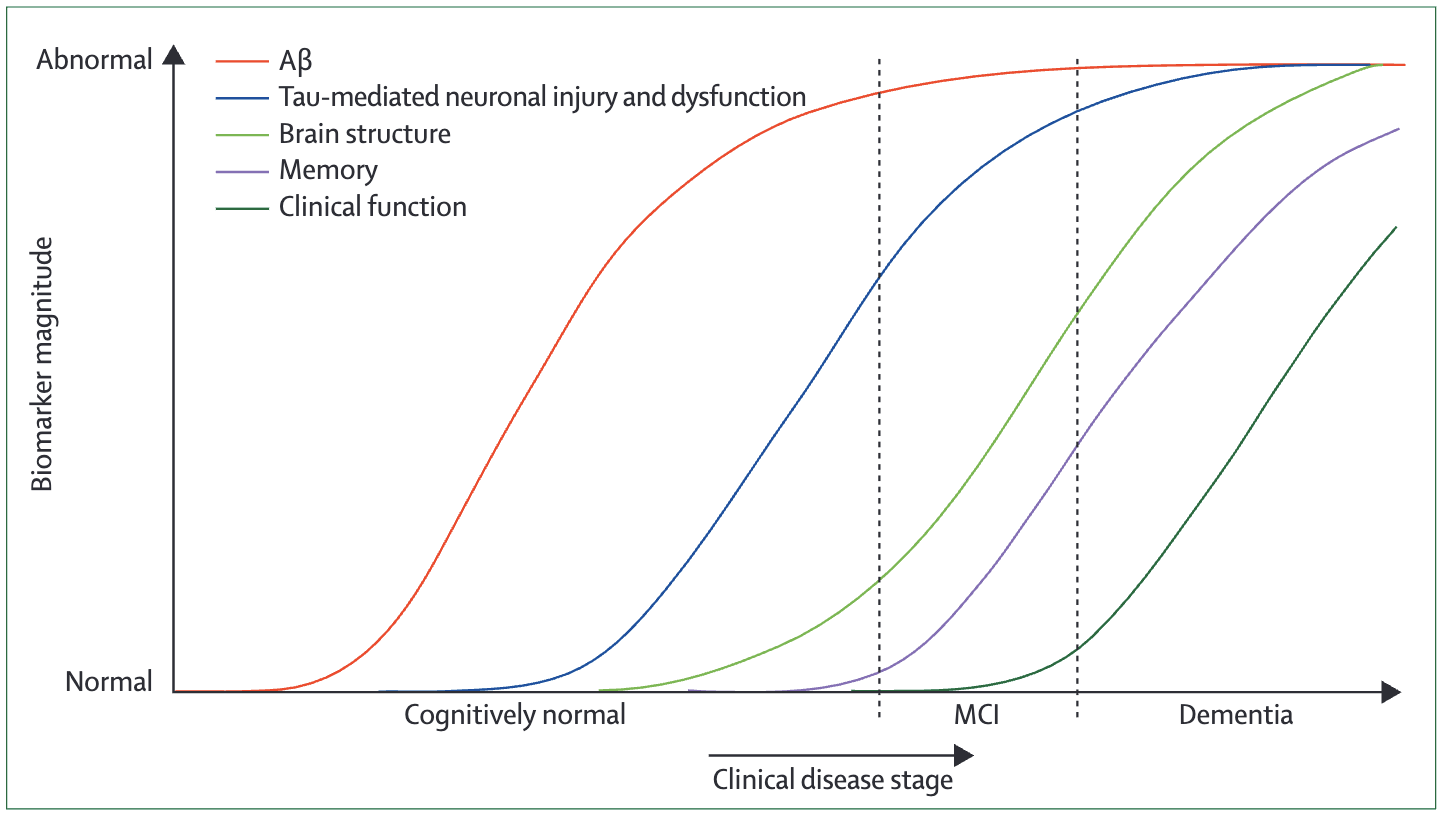
\includegraphics[width=\textwidth]{figures/biomarkers.png}
  \caption{Temporal progression of AD biomarkers, showing the relative timeline of pathophysiological changes~\cite{jack2013tracking}.}
  \label{fig:biomarker_progression}
\end{figure}

Hippocampal atrophy represents one of the earliest and most established structural biomarkers in Alzheimer's disease progression~\cite{jack1992mr}. Volume reductions follow a predictable pattern, beginning years before clinical symptoms emerge, with annual atrophy rates of 3-6\% in AD compared to 1-2\% in normal aging~\cite{vemuri2010role}. Volumetric measurements correlate strongly with cognitive decline and Braak staging of neurofibrillary pathology. Standardized quantification methods include manual tracing, automated segmentation, and shape analysis, achieving diagnostic sensitivities of 80-90\% and specificities of 80-95\% in distinguishing AD from healthy controls~\cite{cuingnet2011automatic}.

Beyond volumetric measurements, shape analysis methods capture morphological changes in brain structures~\cite{ferrarini2006shape}, detecting subtle deformations missed by volume alone. Other promising markers include cortical thickness measurements~\cite{gutierrez2009patterns}, white matter integrity via diffusion tensor imaging, functional connectivity patterns, and metabolic alterations detectable through PET imaging~\cite{vemuri2010role}. These diverse markers provide complementary information that may enhance transfer learning models' diagnostic accuracy.

\subsubsection{Current Clinical Approaches and the Role of Structural MRI}

Current AD diagnosis follows NINCDS-ADRDA criteria, integrating clinical assessment, cognitive testing, and biomarker analysis~\cite{dubois2007research}. Visual assessment of neuroimaging suffers from significant inter-reader variability, with diagnostic accuracy dependent on radiologist expertise~\cite{cuingnet2011automatic}. A substantial temporal gap exists between initial pathological changes and clinical manifestation, complicating early intervention~\cite{jack2018nia}. Additionally, clinical diagnostic accuracy ranges from 65-96\%, with lower precision in early disease stages when intervention would be most beneficial~\cite{kloppel2008accuracy}.

Within this diagnostic framework, structural MRI provides objective evidence of neurodegeneration that complements clinical assessment, with hippocampal atrophy serving as a primary biomarker~\cite{dubois2007research}. MRI's advantages include non-invasiveness compared to CSF sampling, absence of radiation exposure unlike PET, wider availability, and lower cost~\cite{vemuri2010role}. However, visual assessment suffers from inter-reader variability and limited sensitivity to subtle changes, with accuracy heavily dependent on radiologist expertise~\cite{kloppel2008accuracy}. These limitations underscore the need for quantitative, automated analysis approaches.

T1-weighted imaging offers optimal gray/white matter contrast that enhances visualization of atrophy patterns characteristic of AD~\cite{herrera2013classification}. The standardized MPRAGE protocol ensures consistent acquisition parameters across centers, facilitating algorithm development. T1-weighted sequences are widely available in clinical settings, requiring shorter acquisition times than specialized alternatives while providing excellent anatomical detail for detecting subtle volumetric changes in regions affected early in disease progression.

\subsection{Deep Learning for Medical Image Analysis}

\subsubsection{Evolution and Challenges of Deep Learning in Neuroimaging}

Machine learning approaches for neuroimaging have evolved dramatically over the past decade~\cite{bari2021comparative}. Early methods relied on hand-crafted features and shallow classifiers such as Support Vector Machines (SVMs), requiring extensive domain knowledge for feature engineering~\cite{cuingnet2011automatic}. These approaches typically processed predefined regions of interest, achieving moderate success but lacking generalizability. The shift to deep learning eliminated manual feature extraction, allowing end-to-end learning directly from volumetric data~\cite{litjens2017survey}. This transition has yielded substantial performance improvements, with convolutional neural networks demonstrating superior classification accuracy while requiring less preprocessing and domain expertise. The evolution reflects a fundamental shift from explicit feature definition to automatic hierarchical feature learning.

However, deep learning approaches for medical imaging face several challenges compared to natural image analysis. Data scarcity is a primary limitation, with medical datasets typically orders of magnitude smaller than natural image collections~\cite{litjens2017survey}. This is exacerbated in neuroimaging where patient cohorts are smaller and annotation requires expertise. Also, most neuroimaging datasets are collected at specialized centers, leading to potential dataset bias.

Class imbalance presents another obstacle, particularly in Alzheimer's datasets where diagnostic categories are often unevenly distributed~\cite{davatzikos2019machine}. Clinical deployment demands model interpretability beyond accuracy metrics, as clinicians require transparency in decision-making processes. Explicable AI methods attempt to address this by identifying brain regions contributing to model decisions.

Validation protocols in neuroimaging require particular attention to prevent data leakage through subject-level rather than scan-level partitioning, an issue frequently overlooked in published studies~\cite{litjens2017survey}.

\subsubsection{Volumetric Approaches for Neuroimaging Analysis}

The analysis of volumetric MRI data presents a fundamental trade-off between 2D and 3D approaches. Two-dimensional methods process brain scans as independent slices, offering computational efficiency and leveraging established architectures pretrained on natural images~\cite{liang2021alzheimer, sarraf2016classification}. However, these approaches inevitably lose spatial context between slices, potentially missing subtle 3D patterns crucial for AD detection~\cite{gunawardena2017applying}. Conversely, 3D CNNs preserve volumetric relationships and capture the entire spatial context of atrophy patterns~\cite{payan2015predicting}, but require substantially more parameters and memory~\cite{yang2021reinventing}. This computational burden necessitates downsampling in resource-constrained environments, creating a direct trade-off between spatial resolution and contextual information preservation.

Table~\ref{tab:2d_vs_3d} summarizes the key trade-offs between 2D and 3D approaches for volumetric neuroimaging analysis.

\begin{table}[htbp]
\centering
\begin{tabular}{|p{3cm}|p{6cm}|p{6cm}|}
\hline
\textbf{Aspect} & \textbf{2D Approaches} & \textbf{3D Approaches} \\
\hline
Memory Efficiency & High; processes individual slices & Low; requires full volume in memory \\
\hline
Spatial Context & Limited to in-slice patterns & Preserves volumetric relationships \\
\hline
Pre-trained Models & Readily available from natural image domains & Limited availability, primarily from video domains \\
\hline
Computational Cost & Lower training and inference times & Higher computational demands \\
\hline
Resolution & Can process higher in-plane resolution & Often requires downsampling \\
\hline
Performance & Moderate, particularly with ensemble approaches & Superior when sufficient data and computational resources are available \\
\hline
\end{tabular}
\caption{Comparison of 2D and 3D approaches for volumetric neuroimaging analysis}
\label{tab:2d_vs_3d}
\end{table}

3D CNNs extend convolutional operations to volumetric data, preserving spatial relationships across all dimensions critical for detecting subtle neuroanatomical changes in AD~\cite{ebrahimi2020introducing}. Early on, succesful 3D convolutional autoencoders for Alzheimer's classification established the value of learning hierarchical spatial features directly from volumetric data~\cite{lian2018hierarchical, payan2015predicting}. Residual networks address the vanishing gradient problem through identity shortcuts, enabling deeper architectures beneficial for capturing hierarchical patterns in volumetric MRI~\cite{wu20223d}. 3D ResNet-18 represents an optimal balance between depth and computational efficiency, containing 33.2M parameters compared to 46.4M in ResNet-34~\cite{ebrahimi2020introducing}. Architectural variants, compared in figure \ref{fig:cnn_architectures}, include MC3 (mixed 2D/3D convolutions) and R(2+1)D (factorizing 3D convolutions into spatial and temporal components, figure \ref{fig:2plus1D}) that maintain performance while reducing computational demands~\cite{wu20223d}. R3D preserves full spatial context across all dimensions, while MC3 and R(2+1)D offer computational efficiency with different approaches to dimensional processing~\cite{tran2018closer}.

\begin{figure}[htbp]
  \centering
  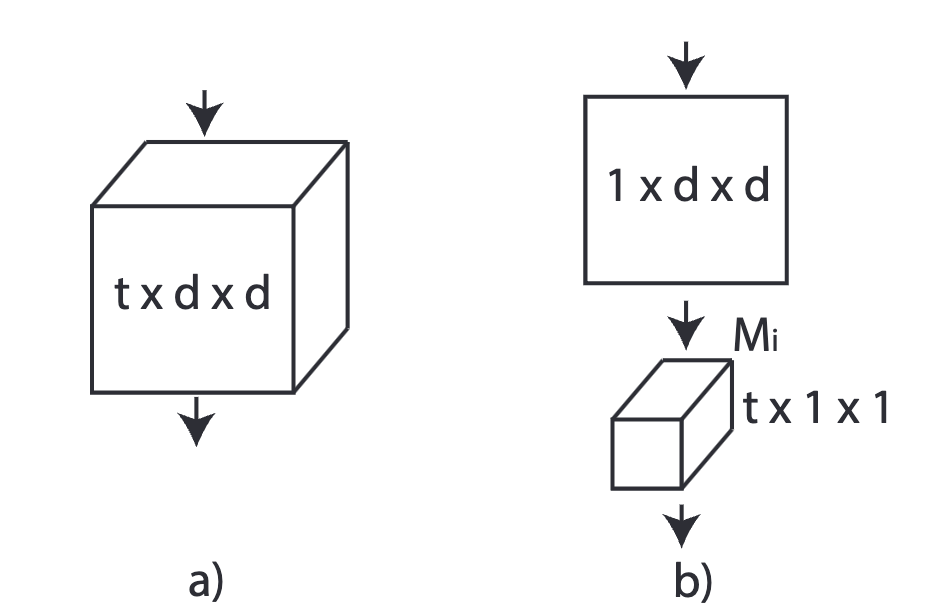
\includegraphics[width=0.5\textwidth]{figures/2plus1d.png}
  \caption{Schematic of R(2+1)D factorized convolutions. (a) being usual 3d convolutions, (b) the R(2+1)D convolutions~\cite{tran2018closer}.}
  \label{fig:2plus1D}
\end{figure}

\begin{figure}[htbp]
  \centering
  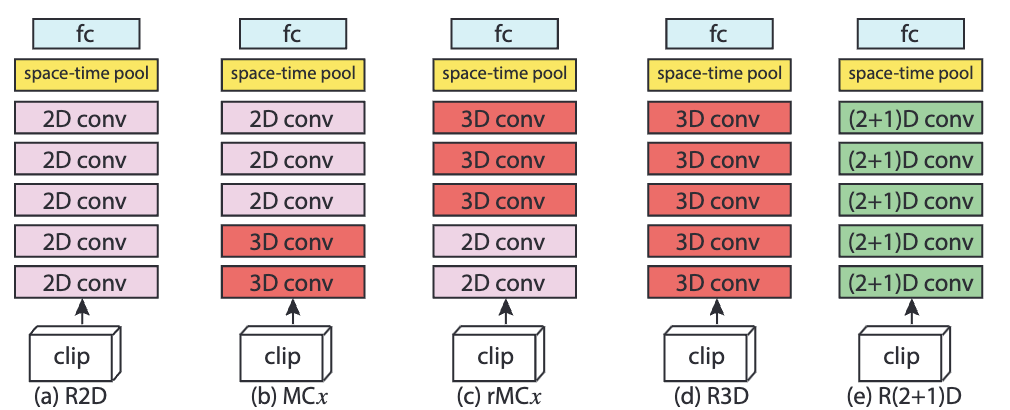
\includegraphics[width=\textwidth]{figures/res_net_archs.png}
  \caption{Schematic comparison of ResNet architectures. We will focus on (a) R3D (fully 3D convolutions), (b) MC3 (mixed 2D/3D convolutions), and (c) R(2+1)D (factorized convolutions)~\cite{tran2018closer}.}
  \label{fig:cnn_architectures}
\end{figure}

Vision Transformers (ViTs) have been adapted to volumetric medical imaging by extending self-attention mechanisms to capture 3D spatial relationships~\cite{lyu2022classification}. Yan et al. demonstrated that hybrid architectures combining CNN and transformer components (Hybrid-RViT) leverage both local feature extraction and global context modeling, outperforming pure CNN or transformer approaches for Alzheimer's detection~\cite{yan2025hybrid}. Despite their capacity to model long-range dependencies, volumetric transformers face computational challenges due to quadratic complexity with input size. Recent efficient transformer variants address these limitations through sparse attention patterns and hierarchical designs~\cite{lu2025efficient}.

Table~\ref{tab:architecture_comparison} compares key architectural approaches for volumetric neuroimaging analysis.

\begin{table}[htbp]
\centering
\begin{tabular}{|p{3cm}|p{5cm}|p{5cm}|}
\hline
\textbf{Architecture} & \textbf{Advantages} & \textbf{Limitations} \\
\hline
3D ResNet & Well-established, efficient parameter usage, strong local feature extraction & Limited receptive field, may miss long-range relationships \\
\hline
MC3 & Balance of efficiency and performance, effective knowledge transfer from video domain & Primarily captures local features, limited global context \\
\hline
R(2+1)D & Increased non-linearities through factorized convolutions, parameter efficiency & Additional computational overhead from factorization \\
\hline
Vision Transformer & Excellent global context modeling, captures long-range dependencies & High computational cost, requires large datasets \\
\hline
Hybrid CNN-ViT & Combines local feature extraction with global context modeling & Complex architecture, more hyperparameters to tune \\
\hline
\end{tabular}
\caption{Comparison of architectural approaches for volumetric neuroimaging analysis}
\label{tab:architecture_comparison}
\end{table}

The conceptual similarity between video sequences and volumetric medical data enables innovative transfer learning approaches. In videos, the temporal dimension captures motion patterns, while in 3D MRI, the depth dimension encodes spatial relationships~\cite{tran2018closer}. Models like MC3, R(2+1)D, and r3d\_18 pre-trained on large video datasets like Kinetics-400 can be fine-tuned for MRI classification by treating the axial dimension as analogous to time~\cite{ebrahimi2020introducing, tran2018closer}.

The adaptation process requires careful consideration of domain differences. Motion patterns in videos have no direct relation to static MRI volumes, necessitating fine-tuning strategies that adapt pretrained feature extractors to the neuroimaging domain.

\subsubsection{Transfer Learning in Medical Imaging}

Transfer learning addresses data scarcity in medical imaging by leveraging knowledge from models pretrained on large datasets~\cite{hon2017towards}. This approach is particularly valuable for neuroimaging applications where annotated data is limited~\cite{ebrahimi2019transfer}. When applying transfer learning to medical domains, researchers must navigate significant domain shifts between natural images and medical scans~\cite{mehmood2021transfer}.

Transfer learning strategies for medical imaging include:
\begin{enumerate}
\item \textbf{Natural image transfer:} Models pretrained on ImageNet are adapted to 2D medical slices~\cite{maqsood2019transfer}.
\item \textbf{Cross-modality transfer:} Knowledge from one imaging modality is transferred to another~\cite{yang2020mri, kieselmann2021cross}.
\item \textbf{Video-to-volumetric transfer:} Models pretrained on video datasets are adapted to 3D medical volumes~\cite{wu20223d}.
\item \textbf{Self-supervised pretraining:} Models are pretrained on unlabeled medical data using proxy tasks~\cite{tang2022self}.
\end{enumerate}

For Alzheimer's detection, researchers have explored ImageNet pretrained models using 2D slice-based methods~\cite{hon2017towards,maqsood2019transfer}, and more recently, 3D volumetric techniques with transfer from video classification models~\cite{ebrahimi2020introducing}, which shows promise due to architectural parallels between spatiotemporal video data and volumetric MRI.

To adapt pretrained models, early layers are frozen to retain low-level features while fine-tuning deeper layers for domain-specific patterns~\cite{acharya2021alzheimer}. The effectiveness of different freezing strategies depends on the similarity between source and target domains.

\subsubsection{Performance Comparisons from Existing Literature}

Benchmark studies show considerable variation in reported performance metrics. Cuingnet et al.'s seminal comparison demonstrated sensitivity ranging from 67-81\% and specificity from 68-95\% for AD versus controls using the ADNI dataset~\cite{cuingnet2011automatic}. More recent deep learning approaches report substantially higher accuracy (85-98\%), with 3D CNN architectures generally outperforming 2D approaches when properly validated~\cite{basaia2019automated, garg2023review}.

However, critical methodological analyses have revealed that many studies suffer from data leakage through scan-level rather than subject-level partitioning, potentially inflating performance by 10-15\%~\cite{davatzikos2019machine}. When accounting for proper subject isolation, performance metrics typically show more modest improvements over traditional methods.

\subsection{MRI Preprocessing for Deep Learning}

\subsubsection{Skull Stripping and Registration Approaches}

Skull stripping, the isolation of brain tissue from surrounding structures, represents a critical preprocessing step~\cite{fatima2020state}. Learning-based approaches like SynthStrip demonstrate superior robustness across imaging protocols and pathological conditions~\cite{hoopes2022synthstrip}. SynthStrip particularly excels with neurodegenerative cases, where traditional methods like intensity-based thresholding often fail due to enlarged ventricles and cortical atrophy, see figure \ref{fig:skull_stripping}.

\begin{figure}[htbp]
  \centering
  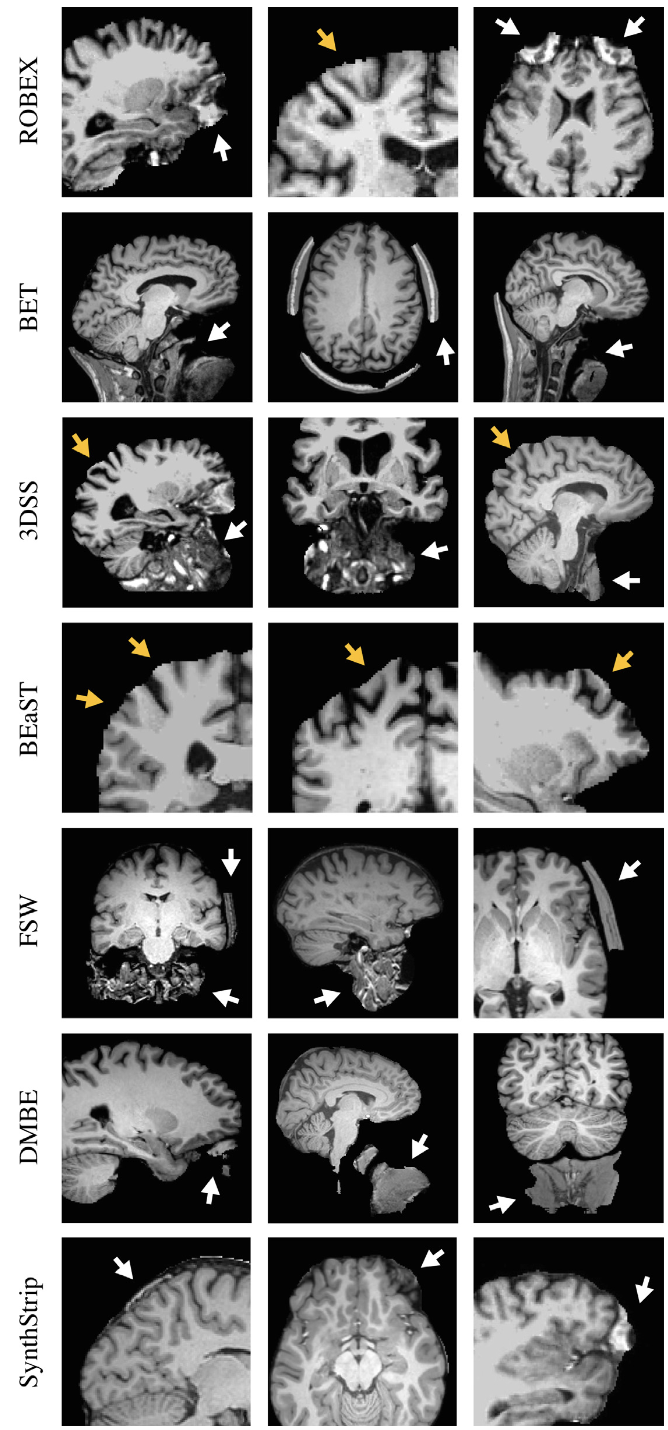
\includegraphics[width=0.33\textwidth]{figures/ss_fails.png}
  \caption{Example of common failures of skull stripping methods. We can see how the minor mistakes synthstrip commits do not crop the brain structure like more primitive methods do~\cite{hoopes2022synthstrip}}
  \label{fig:skull_stripping}
\end{figure}

Registration to standardized templates (e.g., MNI152) normalizes anatomical variability, facilitating voxel-wise comparisons across subjects~\cite{garg2023review}. However, registration presents a trade-off between standardization and preservation of pathology-specific features. While traditional machine learning approaches typically benefit from rigorous registration, deep learning methods can achieve superior performance with minimal registration that preserves native anatomical features by learning invariant representations, potentially extracting diagnostic patterns despite anatomical variability.

While normalization improves model interpretability by establishing spatial correspondence~\cite{viswan2025enhancing}, excessive regularization risks attenuating the volumetric changes characteristic of AD. Intensity normalization addresses scanner-specific variations, with Z-score normalization particularly effective for deep learning applications by constraining gradient magnitudes during training~\cite{viswan2025enhancing}.

\subsubsection{Impact of Preprocessing on Model Performance}

Preprocessing significantly impacts deep learning performance for AD detection. Viswan et al. demonstrated that proper preprocessing pipelines can improve classification accuracy by 5-15\% compared to minimal preprocessing~\cite{viswan2025enhancing}. Skull stripping shows the most substantial impact, with improperly stripped volumes reducing accuracy by up to 8\%. Registration demonstrates a more nuanced effect—while standardizing anatomical positioning enhances performance for shallow classifiers, deep networks can sometimes perform better with unregistered data preserving native atrophy patterns. Intensity normalization consistently improves performance by 3-7\% across architectures by mitigating scanner variability.

Table~\ref{tab:preprocessing_impact} summarizes the impact of different preprocessing steps on model performance.

\begin{table}[htbp]
\centering
\begin{tabular}{|p{3cm}|p{5cm}|p{5cm}|p{2cm}|}
\hline
\textbf{Preprocessing Step} & \textbf{Implementation Approach} & \textbf{Effect on Performance} & \textbf{Relative Impact} \\
\hline
Skull Stripping & Learning-based (SynthStrip) & Eliminates confounding signals, improves feature extraction precision & High (+5-8\%) \\
\hline
Registration & Affine only (preserving some atrophy patterns) & Standardizes orientation while preserving disease-specific features & Moderate (+2-5\%) \\
\hline
Intensity Normalization & Z-score normalization & Mitigates scanner variability, constrains gradient magnitudes & Moderate (+3-7\%) \\
\hline
Bias Field Correction & N4 algorithm & Reduces intensity non-uniformity artifacts & Low-Moderate (+1-3\%) \\
\hline
\end{tabular}
\caption{Impact of preprocessing steps on model performance for AD classification}
\label{tab:preprocessing_impact}
\end{table}

\subsubsection{Data Partitioning and Group Leakage Prevention}
\label{subsec:data_partitioning}

Data leakage represents a critical methodological concern in neuroimaging studies, occurring when information from test samples inadvertently influences model training. This issue is particularly problematic in longitudinal neuroimaging datasets with multiple scans from the same subject across different timepoints~\cite{davatzikos2019machine}.

Subject-level partitioning—ensuring all scans from an individual remain exclusively in either training, validation, or test sets—is essential for preventing "group leakage." In contrast, scan-level partitioning (where different scans from the same subject may appear in both training and test sets) can dramatically overestimate model performance by 10-15\% in classification accuracy~\cite{davatzikos2019machine}.

Many published neuroimaging studies fail to clearly report their data partitioning methodology, making it difficult to assess the validity of reported performance metrics. This has led to a growing emphasis on methodological transparency and rigorous validation protocols in recent literature~\cite{davatzikos2019machine}.

\subsection{Current State of the Art and Research Gaps}

\subsubsection{Recent Advances in Automated AD Detection}

Recent years have seen significant progress in automated Alzheimer's disease detection using deep learning. Convolutional neural networks have emerged as the dominant methodology, with 3D architectures demonstrating superior performance. Early approaches achieved strong accuracy using 2D CNN ensembles~\cite{farooq2017deep}, then transfer learning to 3D ResNet-18 was introduced, leveraging pre-trained weights to achieve 96.88\% accuracy despite limited training data~\cite{ebrahimi2020introducing}.Vision Transformers (ViTs) represent the newest architectural innovation, with hybrid CNN-transformer models demonstrating state-of-the-art performance. Current performance benchmarks for binary AD classification range from 85-98\% accuracy, with 3D approaches consistently outperforming 2D counterparts~\cite{saikia2024alzheimer,mubonanyikuzo2025detection}. However, it is unclear whether these account for proper subject-level validation.

Despite these advances, several challenges remain. Data scarcity limits model training~\cite{pradhan2024analysis}, while heterogeneous MRI acquisition protocols introduce variability that complicates model generalization. Adapting video classification architectures to 3D MRI data requires substantial modifications that may compromise the benefits of pre-trained weights. The "black box" nature of deep learning models raises concerns about clinical interpretability and trustworthiness~\cite{basaia2019automated}. Lastly, domain shift between source and target tasks remains problematic, potentially limiting the effectiveness of knowledge transfer from non-medical to medical imaging applications.

\subsubsection{Research Gap Addressed by This Work}

Despite advances in deep learning for Alzheimer's detection, several key methodological and technical gaps remain that this work aims to address:

\begin{enumerate}
\item \textbf{Volumetric transfer learning:} The adaptation of pretrained 3D models for volumetric medical imaging remains underexplored. This work systematically investigates the effectiveness of video-pretrained models for AD classification.

\item \textbf{Methodological rigor:} Many published studies suffer from methodological flaws including scan-level partitioning. This research implements rigorous subject-level validation methodology.

\item \textbf{Preprocessing optimization:} The impact of different preprocessing choices on transfer learning performance is incompletely understood. This work develops an optimized pipeline specifically designed to preserve diagnostically relevant features.

\item \textbf{Architectural comparison:} Limited research exists comparing architectures specifically optimized for video classification on neuroimaging tasks. This study evaluates these variants to determine the optimal approach for volumetric MRI analysis.
\end{enumerate}

These research gaps directly inform the methodology in the next section, which implements a rigorous experimental framework to evaluate video-pretrained model transfer for Alzheimer's disease detection.

\section{Methodology}
\label{sec:methodology}

\subsection{Data Acquisition and Characteristics}

The Alzheimer's Disease Neuroimaging Initiative (ADNI) database served as the primary data source, providing standardized MRI acquisitions with corresponding clinical diagnoses. ADNI was selected over alternatives (including OASIS) for its comprehensive coverage, acquisition protocols, and expert-validated diagnoses~\cite{jack2008alzheimer, lamontagne2019oasis}.

\subsubsection{Dataset Composition}

All selected scans were T1-weighted MPRAGE sequences (1.5T or 3T, 1mm³ isotropic resolution), chosen for optimal gray/white matter contrast, standardized acquisition parameters, and sensitivity to atrophy biomarkers. Additionally, the widespread clinical availability and established role of MPRAGE in AD assessment made it an ideal choice for this study. The final dataset contained 1,300 scans from 408 unique subjects, balanced between diagnostic categories:

\begin{table}[htbp]
\centering
\begin{tabular}{|l|c|c|}
\hline
\textbf{Partition} & \textbf{AD} & \textbf{CN} \\
\hline
Training & 512 scans (133 subjects) & 511 scans (115 subjects) \\
Validation & 69 scans (35 subjects) & 70 scans (45 subjects) \\
Test & 69 scans (35 subjects) & 69 scans (45 subjects) \\
\hline
\end{tabular}
\caption{Distribution of scans and subjects across dataset partitions}
\end{table}

\subsubsection{Diagnostic Criteria}

Subjects were classified as Alzheimer's Disease (AD) or Cognitively Normal (CN) based on NINCDS-ADRDA criteria. Initially, the dataset contained $\sim$33\% AD and $\sim$67\% CN cases. To address class imbalance and potential overfitting issues identified during preliminary experiments, additional AD scans were incorporated and CN subjects carefully sampled to achieve a balanced 50/50 diagnostic distribution.

The binary classification focus (excluding Mild Cognitive Impairment) reflects the clearer structural changes observable in established AD, particularly hippocampal atrophy, which serves as a primary biomarker for disease progression. Subject-level isolation between dataset partitions was strictly enforced to prevent data leakage, ensuring realistic performance assessment for unseen individuals.

\subsection{Preprocessing Pipeline}

\subsubsection{Initial Processing and Skull Stripping}

Raw DICOM images were converted to NIfTI format using \texttt{dicom2nifti} with reorientation and compression enabled. This created unified volumetric files suitable for 3D analysis. Skull stripping was performed using SynthStrip, a deep learning-based method that represents the current state-of-the-art for brain extraction~\cite{hoopes2022synthstrip}. It was selected for its superior performance with atrophied brains. Unlike traditional threshold-based methods (e.g., BET), SynthStrip preserved critical cortical boundaries even with atrophied brains and better handled the variability in the ADNI dataset. Despite requiring $\sim$2.5 minutes per scan, the improved quality justified this approach by preventing potential misinterpretation of artifacts as disease-related changes.

\subsubsection{Volume Standardization}

All volumes were resampled to isotropic 1×1×1mm voxels using ANTs with third-order spline interpolation. This standardization ensured consistent spatial representation, eliminated scanner-specific resolution variability, and enabled uniform convolutional filter operations across all dimensions.

\subsubsection{Adaptive Cropping Strategy}

A key methodological innovation was the implementation of an adaptive cropping procedure followed by reshaping to 128×128×128 dimensions. The approach:

\begin{enumerate}
    \item Identified brain-containing regions using intensity thresholding
    \item Applied cropping with minimal padding (3 voxels)
    \item Used cubic interpolation to reach the target dimensions
\end{enumerate}
% TODO add appendix to crop brain from mri function

This method preserved $\sim$35\% more effective resolution for critical structures like the hippocampus compared to naive downsampling. The 128³ dimension balanced preserving anatomical detail with memory constraints for model training. The original uncropped 96³ images compared to the cropped 128³ images are shown in figure \ref{fig:cropping}.
\begin{figure}[htbp]
  \centering
  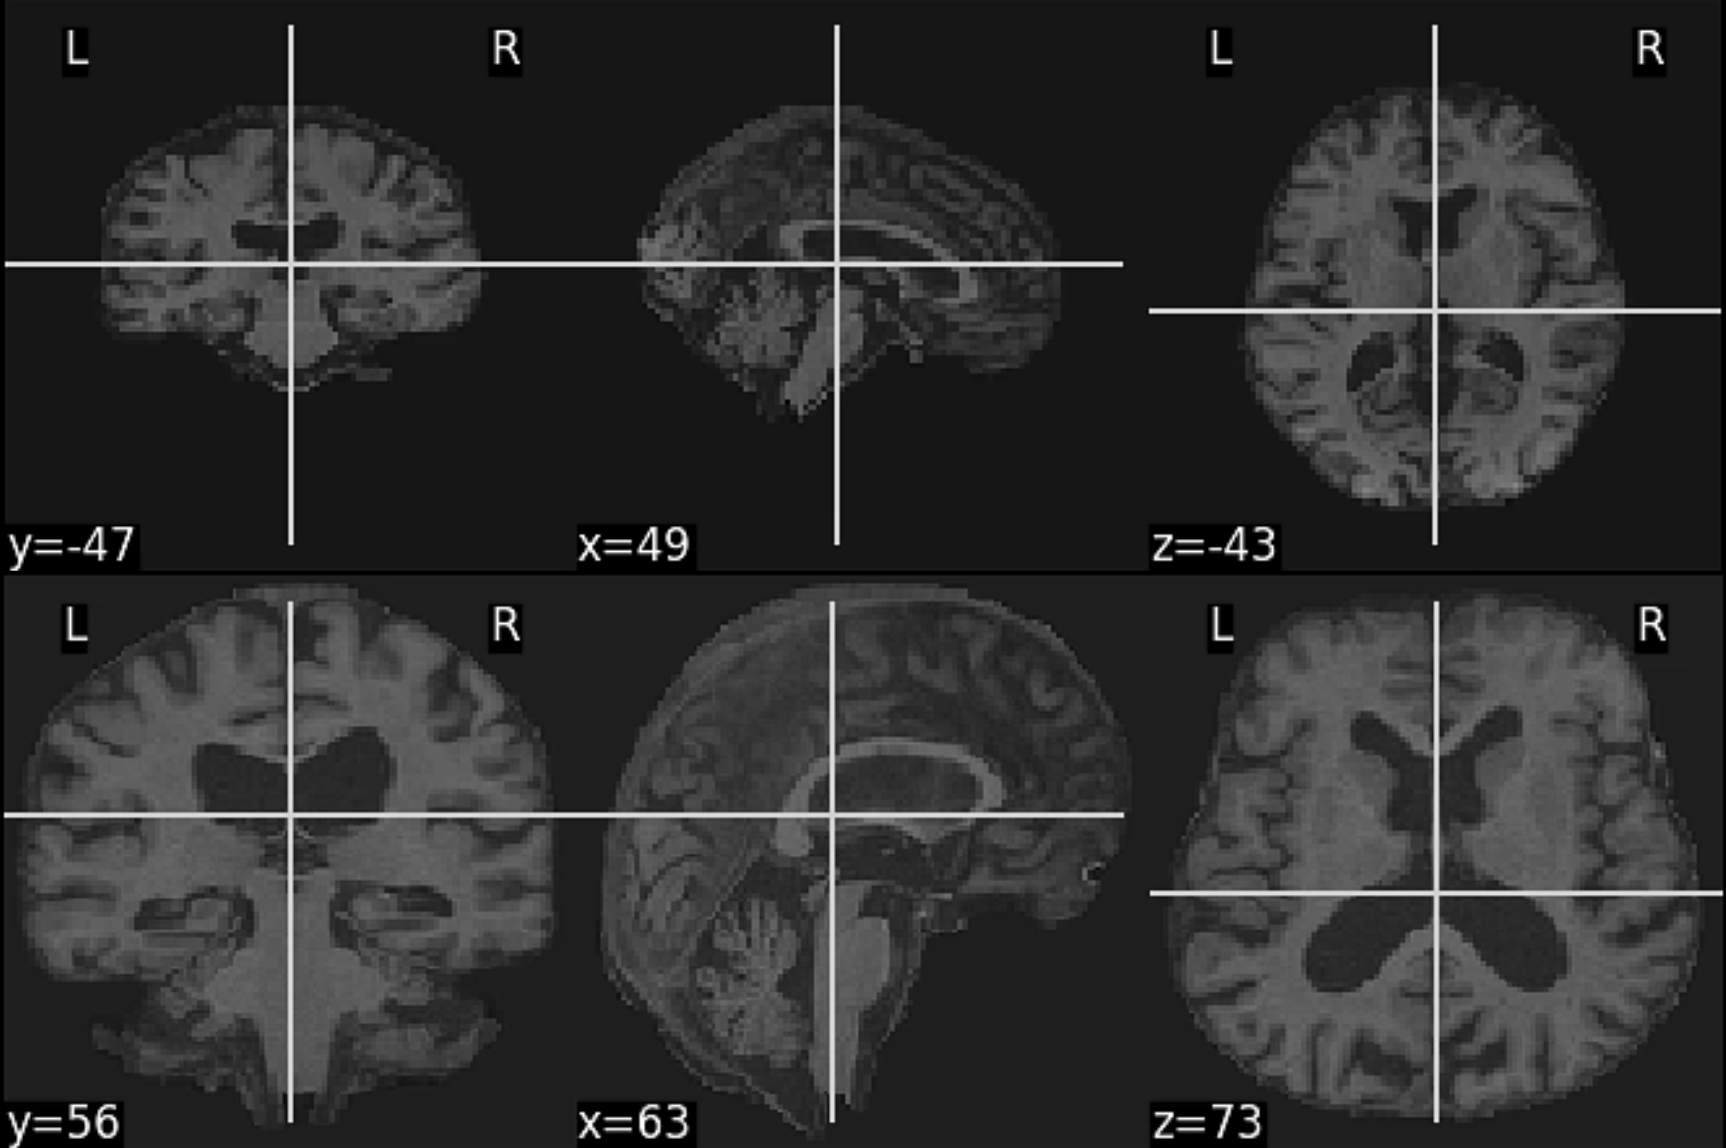
\includegraphics[width=0.8\textwidth]{figures/cropping.png}
  \caption{Comparison of original 96³ (top) and cropped 128³ (bottom) images. The cropping process preserves critical anatomical features while reducing irrelevant background.}
  \label{fig:cropping}
\end{figure}

\subsubsection{Intensity Normalization and Orientation}

N4 bias field correction was applied to mitigate intensity inhomogeneities from magnetic field variations. This prevents intensity variations that might be misinterpreted as structural changes. All volumes were reoriented to Right-Anterior-Superior (RAS) orientation to ensure consistent directionality, allowing the model to focus solely on relevant structural differences rather than arbitrary orientation variations.
% TODO reference code from appendix

\subsubsection{Omission of Spatial Normalization}

Despite its common use in neuroimaging pipelines, registration to standard space (e.g., MNI152) was deliberately omitted for several reasons. Preservation of native atrophy patterns that could be distorted during normalization was a primary consideration. The approach also relied on CNN translation invariance to identify structures without explicit alignment. Additionally, avoiding interpolation artifacts that might smooth critical structural boundaries was important for maintaining diagnostic features.

Validation experiments confirmed that models trained on native-space data performed comparably to or better than those using normalized data, supporting this methodological decision and aligning with recent literature suggesting deep learning models for brain MRI benefit from native-space learning.

The entire pipeline produced 1,300 preprocessed volumes with consistent dimensions, orientation, and intensity characteristics while preserving the structural variations essential for AD classification.

\subsubsection{Data Splitting Strategy}

A methodologically rigorous data splitting approach was implemented to prevent data leakage while maintaining diagnostic balance across partitions. Unlike conventional image classification tasks, neuroimaging datasets require subject-level rather than scan-level splitting since multiple scans often exist for the same individual.

A strict subject-level isolation approach ensured no individual appeared in multiple dataset partitions—a critical decision after initial experiments revealed artificially inflated performance metrics ($\sim$90\% accuracy) when subjects were allowed to cross partition boundaries. Complete subject isolation produced a more realistic performance assessment ($\sim$77\% accuracy), better reflecting the model's generalization capability to unseen individuals.

To prevent subtle forms of data leakage, preprocessing parameters (such as intensity normalization statistics) were computed independently within each partition. This methodologically sound approach ensured that performance metrics would accurately reflect the model's ability to generalize to entirely new individuals, rather than merely recognizing previously seen subjects in different scans.

The dataset was divided following an 80/10/10 (train/validation/test) ratio using a round-robin algorithm that:
\begin{enumerate}
    \item Grouped subjects by diagnostic condition
    \item Sorted subjects in ascending order by scan count
    \item Allocated subjects to partitions round robin to insure subject diversity across partitions
    \item Final scan counts were balanced to maintain equal scan counts per diagnostic category
\end{enumerate}

This approach yielded a balanced distribution with 1,023 training scans (512 AD/511 CN), 139 validation scans (69 AD/70 CN), and 138 test scans (69 AD/69 CN). The strict isolation maintained 203 unique subjects in training, 80 in validation, and 80 in test sets, with diagnostic balance preserved in each partition.

\subsection{Data Augmentation}

Data augmentation was strategically implemented to improve model generalization while preserving diagnostically relevant features. Through systematic experimentation, a minimal yet effective set of transformations was identified:

\begin{verbatim}
tio.Compose([
    tio.RandomNoise(mean=0.0, std=0.1, p=0.3),
    tio.RandomGamma(log_gamma=(-0.2, 0.2), p=0.3),
    tio.ZNormalization(),
])
\end{verbatim}

This approach was applied exclusively to the training set, while validation and test sets received only Z-normalization to maintain evaluation consistency. In practice I saw a 5\% improvement in test accuracy, and consistent improvement in validation accuracy as seen in figure \ref{fig:normalisation_accuracy}.

Each technique addressed specific neuroimaging considerations: Random noise (30\% probability, $\sigma$=0.1) simulated scanner variability and promoted robustness to image quality differences; Gamma adjustment (±0.2 range, 30\% probability) mimicked contrast variations between scanners; Z-normalization standardized intensity values across all scans for consistent feature extraction.

Notably, common augmentation techniques were deliberately excluded after experimental evaluation. Geometric transformations such as rotations and flips significantly increased training time (from approximately 5 to 20 epochs) without improving validation accuracy, likely due to inherent orientation variability already present in MRI data. Similarly, random scaling (0.9-1.1) showed no generalization improvement and potentially disrupted the carefully standardized voxel dimensions established during preprocessing.

The final strategy evolved from extensive transformations to this focused set through iterative evaluation of validation performance and convergence speed, representing an optimal balance between enhancing robustness and preserving critical structural features essential for AD classification.
\subsection{Model Development and Training}
\subsubsection{Model Architecture}

The primary model was a modified 3D ResNet-18 (r3d\_18), the implementation used PyTorch's pre-trained r3d\_18 model, with the first layer modified to accept single-channel MRI volumes and the final layer adapted for binary classification. The model architecture consisted of 18 layers, with the first layer being a 3D convolutional layer followed by four residual blocks, each containing two 3D convolutional layers. The final fully connected layer was adapted to output binary classification scores.

The model was trained using a transfer learning approach, leveraging pre-trained weights from the Kinetics400 dataset, which provided a strong initialization for the feature extraction layers. Early convolutional layers (25\% of parameters) were frozen while allowing the final residual block and fully connected layer (75\%) to adapt to MRI-specific features. This balanced preserving pre-trained knowledge with domain adaptation. Initial experiments with more aggressive freezing (keeping only the final fully connected layer trainable) resulted in numerical instabilities during training, manifested as NaN losses, suggesting that significant domain adaptation was necessary given the substantial differences between video action recognition and MRI classification.

A differential learning rate strategy applied a 10× higher learning rate to the newly initialized fully connected layer compared to the fine-tuned convolutional layers, enabling aggressive adaptation in the task-specific output layer while making more conservative updates to the pre-trained feature extraction layers.
% TODO add learning rates code in appendix

The final model architecture parameters were:

\begin{itemize}
    \item \textbf{Total parameters}: 33,148,482
    \item \textbf{Trainable parameters}: 24,909,826 (75.15\%)
    \item \textbf{Frozen parameters}: 8,238,656 (24.85\%)
\end{itemize}

These figures represent a significant reduction compared to larger architectures like ResNet-50 or ViT variants, making training feasible on consumer-grade hardware while maintaining sufficient capacity for the classification task. The reduced parameter count also potentially mitigated overfitting given the relatively small dataset size.

\subsubsection{Architecture Comparison}

To validate architectural choices, models were systematically evaluated with decreasing levels of 3D feature extraction. The Mixed Convolution 3D Network (MC3-18) uses a hybrid approach combining 2D and 3D convolutions, hypothesized to potentially offer computational efficiency while maintaining performance. Experimental results with MC3-18 showed less stable training dynamics and inferior performance compared to the pure 3D approach of R3D-18, supporting the importance of fully volumetric feature extraction for structural MRI analysis. The differences in performance provided empirical justification for the primary architectural choice.

Following the investigation of MC3-18, a (2+1)D architecture was also evaluated. This approach decomposes 3D convolutions into separate spatial (2D) and temporal (1D) convolutions, a technique that has shown promise in video classification tasks. Results with the (2+1)D architecture revealed performance that was slightly worse than MC3-18, continuing the observed trend that classification accuracy decreased as the model architecture incorporated more 2D elements. This progression (R3D > MC3 > (2+1)D) strongly suggests that preserving the full 3D spatial context through pure 3D convolutions is critical for detecting the subtle volumetric patterns associated with Alzheimer's disease in MRI data.

Recent advances in vision transformers prompted investigation of their potential for 3D MRI classification. However, initial implementation attempts revealed significant computational barriers. Memory requirements exceeded available hardware capabilities (32GB RAM requirement for 128×128×128 volumes). There was also architectural mismatch between the input dimensions required by MViT (designed for 16×224×224 video clips) and the cubical 128×128×128 MRI volumes. Additionally, transformer architectures typically require substantially larger training datasets than were available. These constraints prevented full evaluation of transformer-based approaches, highlighting an important practical limitation in applying state-of-the-art vision models to medical imaging with limited computational resources.

\subsubsection{Training Framework and Implementation}

Training was conducted on an M1 Mac using Metal Performance Shaders, with each epoch requiring approximately one hour and full training runs taking $\sim$20 hours. This hardware constrained batch size and architecture selection. Despite attempts at optimization through mixed precision training and CPU-GPU synchronization, computational bottlenecks in the model's forward pass remained.

Hyperparameters were selected through systematic experimentation and tracked with Weights \& Biases:

\begin{table}[htbp]
\centering
\begin{tabular}{|l|l|p{5.5cm}|}
\hline
\textbf{Parameter} & \textbf{Value} & \textbf{Rationale} \\
\hline
Learning rate & 0.001 (FC), 0.0001 (conv) & Differential rates for aggressive output adaptation with conservative updates to pre-trained layers \\
\hline
Optimizer & AdamW (weight decay=0.01) & Effective regularization for the limited dataset \\
\hline
Batch size & 2 & Memory constraints from 128³ inputs \\
\hline
LR schedule & Cosine annealing ($T_0$=5) & Prevents convergence to local minima \\
\hline
\end{tabular}
\caption{Optimized hyperparameter configuration}
\end{table}

A weighted cross-entropy loss function addressed potential class imbalance with weights dynamically calculated based on class distribution, particularly important during initial experiments when the dataset had not yet been fully balanced. This ensured balanced contribution to loss regardless of class representation.

% TODO add to appendix

Early stopping with patience=5 monitored both validation accuracy and loss, ensuring training continued as long as either metric showed enhancement, preventing overfitting while optimizing computational resources. Most models converged within 5-10 epochs, with early stopping typically triggering around epoch 7-8—quick convergence attributable to the transfer learning initialization.

A comprehensive checkpoint system saved regular epoch checkpoints and best models based on both accuracy and loss metrics. Each checkpoint stored model weights, optimizer state, scheduler state, and performance metrics for seamless training resumption. The system integrated with Weights \& Biases to log best models as artifacts.

The training loop was implemented with careful attention to numerical stability and memory management. Memory optimization techniques included setting gradients to \texttt{None} rather than zero (reducing memory fragmentation) and using tensor operations that maintained computational efficiency. For MPS acceleration, explicit cache clearing was performed at the end of each epoch to prevent memory accumulation.

\subsection{Evaluation Methodology}

\subsubsection{Performance Metrics}

A comprehensive set of metrics was implemented to evaluate model performance beyond simple accuracy:

\begin{itemize}
    \item \textbf{Accuracy and balanced accuracy}: The latter particularly important for medical applications as it equalizes the contribution of each diagnostic class.
    
    \item \textbf{Precision and recall}: Critical for clinical utility, measuring correct positive predictions and the ability to identify true AD cases, respectively.
    
    \item \textbf{Specificity}: Quantified the model's ability to correctly identify CN cases ($TN/(TN+FP)$).
    
    \item \textbf{F1-score, ROC-AUC, and average precision}: Provided threshold-independent performance assessment.
\end{itemize}

All metrics were continuously tracked and logged using a custom \texttt{MetricsManager} class, with implementation details provided in Appendix X.
% TODO add to appendix

\subsubsection{Evaluation Framework and Validation Strategy}

The evaluation framework employed strict subject-level isolation to prevent data leakage. Dedicated validation (10\%) and test (10\%) sets maintained complete separation from training data, with no subjects appearing in multiple partitions. To mitigate selection bias and ensure robust model evaluation, multiple model checkpoints were saved throughout training, including both the best accuracy and best loss models. This approach provided resilience against overfitting to particular validation set characteristics. For final performance assessment, only the held-out test set was used with the best validation accuracy checkpoint, maintaining complete independence between model selection and final evaluation to ensure unbiased performance estimates.


Statistical rigor was ensured through comprehensive uncertainty quantification and comparative analysis. Bootstrap confidence intervals were calculated for key performance metrics, providing a robust quantification of the uncertainty in the model's performance estimates. Confusion matrix analysis was performed to identify classification patterns and error types, revealing balanced false positive and false negative distributions. Additionally, the model's performance was contextualized through comparison to multiple baselines, including random chance (50\%), published clinical radiologist performance, and results from existing algorithmic approaches in the literature. These comparative analyses provided important reference points for evaluating the clinical utility and relative advantages of the proposed approach within the broader landscape of AD detection methodologies.


Despite computational constraints with training runs requiring approximately 20 hours on an M1 Mac, model robustness was thoroughly verified through several complementary approaches. Subject-level 3-fold cross-validation was implemented with strict diagnostic balance and complete subject-level isolation maintained across all partitions to ensure reliable performance assessment. Additionally, a systematic architecture comparison across R3D-18, MC3-18, and R2Plus1D-18 models was conducted to assess the impact of dimensional processing on performance and validate the choice of fully 3D convolutional architectures. This comprehensive validation strategy ensured confidence in the model's generalization capabilities despite the computational limitations of the development environment.

% Todo include with xai
% architectures. To supplement these quantitative evaluations, various visualization techniques were employed to provide qualitative insights into model behavior, offering deeper understanding beyond numerical metrics alone. This

\section{Results}
\label{sec:results}

This section presents the quantitative and qualitative results of the proposed transfer learning approach for Alzheimer's disease detection using pre-trained video classification models adapted to MRI analysis. The results demonstrate the effectiveness of 3D convolutional architectures, particularly the R3D-18 model, for identifying structural patterns associated with AD.

\subsection{Model Performance Analysis}

\subsubsection{Classification Performance}

The optimized R3D-18 model achieved a test accuracy of 77.26\% for the binary classification of AD versus CN subjects, with balanced precision and recall metrics. Table \ref{tab:performance_metrics} summarizes the key performance metrics for the final model evaluated on the held-out test set and average over each fold.

\begin{table}[htbp]
\centering
\begin{tabular}{|l|c|}
\hline
\textbf{Metric} & \textbf{Value} \\
\hline
Accuracy & 77.26\% \\
Balanced Accuracy & 77.31\% \\
Precision & 77.1\% \\
Recall (Sensitivity) & 79.29\% \\
Specificity & 75.33\% \\
F1-Score & 77.13\% \\
AUC-ROC & 0.86 \\
\hline
\end{tabular}
\caption{Performance metrics for the R3D-18 model on the held-out test set.}
\label{tab:performance_metrics}
\end{table}

The confusion matrix in Figure \ref{fig:confusion_matrix} shows the distribution of predictions across diagnostic categories, revealing a balanced performance between AD and CN classifications with similar false positive and false negative rates.

\begin{figure}[htbp]
  \centering
  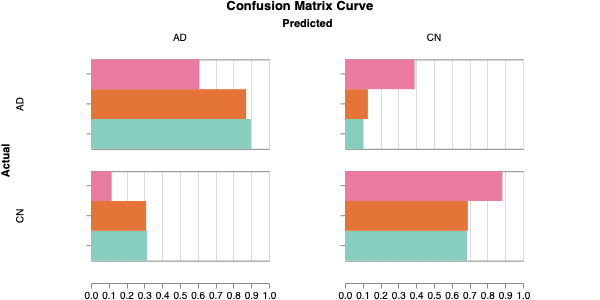
\includegraphics[width=\textwidth]{figures/CM3F.png}
  \caption{Confusion matrix for AD vs CN classification on the test set over 3 folds, showing the distribution of true positives, false positives, true negatives, and false negatives.}
  \label{fig:confusion_matrix}
\end{figure}

\subsubsection{ROC Analysis}

The Receiver Operating Characteristic (ROC) curve in Figure \ref{fig:roc_curve} demonstrates the trade-off between true positive rate and false positive rate across different classification thresholds. With an Area Under the Curve (AUC) of 0.86, it indicates good discriminative ability between AD and CN subjects.

\begin{figure}[htbp]
  \centering
  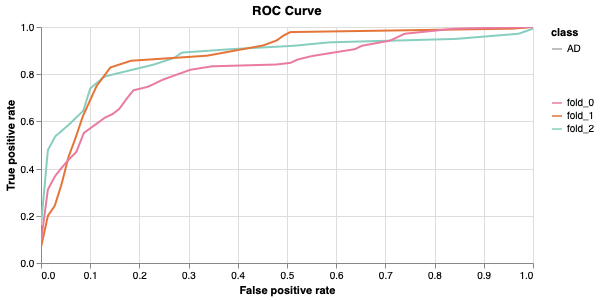
\includegraphics[width=\textwidth]{figures/ROC3F.png}
  \caption{ROC curve for the R3D-18 model on the held out test set over 3 folds. The Area Under the Curve (AUC) is 0.86.}
  \label{fig:roc_curve}
\end{figure}

\subsubsection{Cross-Validation Stability}

To assess model stability and generalization, 3-fold cross-validation was performed with strict subject-level isolation maintained across folds. The results in Table \ref{tab:cross_validation} demonstrate consistent performance across different subject groupings, with a mean accuracy of 77.26\% and standard deviation of 2.34\%.

\begin{table}[htbp]
\centering
\begin{tabular}{|c|c|c|c|c|}
\hline
\textbf{Metric} & \textbf{Fold 1} & \textbf{Fold 2} & \textbf{Fold 3} & \textbf{Mean ± SD} \\
\hline
Accuracy & 79.1\% & 78.01\% & 74.64\% & 77.26 ± 2.34\% \\
\hline
Precision & 73.81\% & 73.49\% & 84.00\% & 77.1 ± 5.98\% \\
\hline
Recall & 89.86\% & 87.14\% & 60.87\% & 79.29 ± 16.01\% \\
\hline
F1-Score & 81.05\% & 79.74\% & 70.59\% & 77.13 ± 5.70\% \\
\hline
\end{tabular}
\caption{3-fold cross-validation results demonstrating model stability across different subject groupings.}
\label{tab:cross_validation}
\end{table}

The low standard deviation (2.34\%) across folds indicates robust performance independent of specific subject allocation, supporting the generalizability of this approach to unseen individuals.

\subsubsection{Learning Curve Analysis}

The learning curves for the R3D-18 model over 3 folds exhibited relatively quick convergence, typically within 4-8 epochs, attributable to the transfer learning initialization. Figure \ref{fig:learning_curves} shows the characteristic progression of training and validation metrics across epochs.

\begin{figure}[htbp]
  \centering
  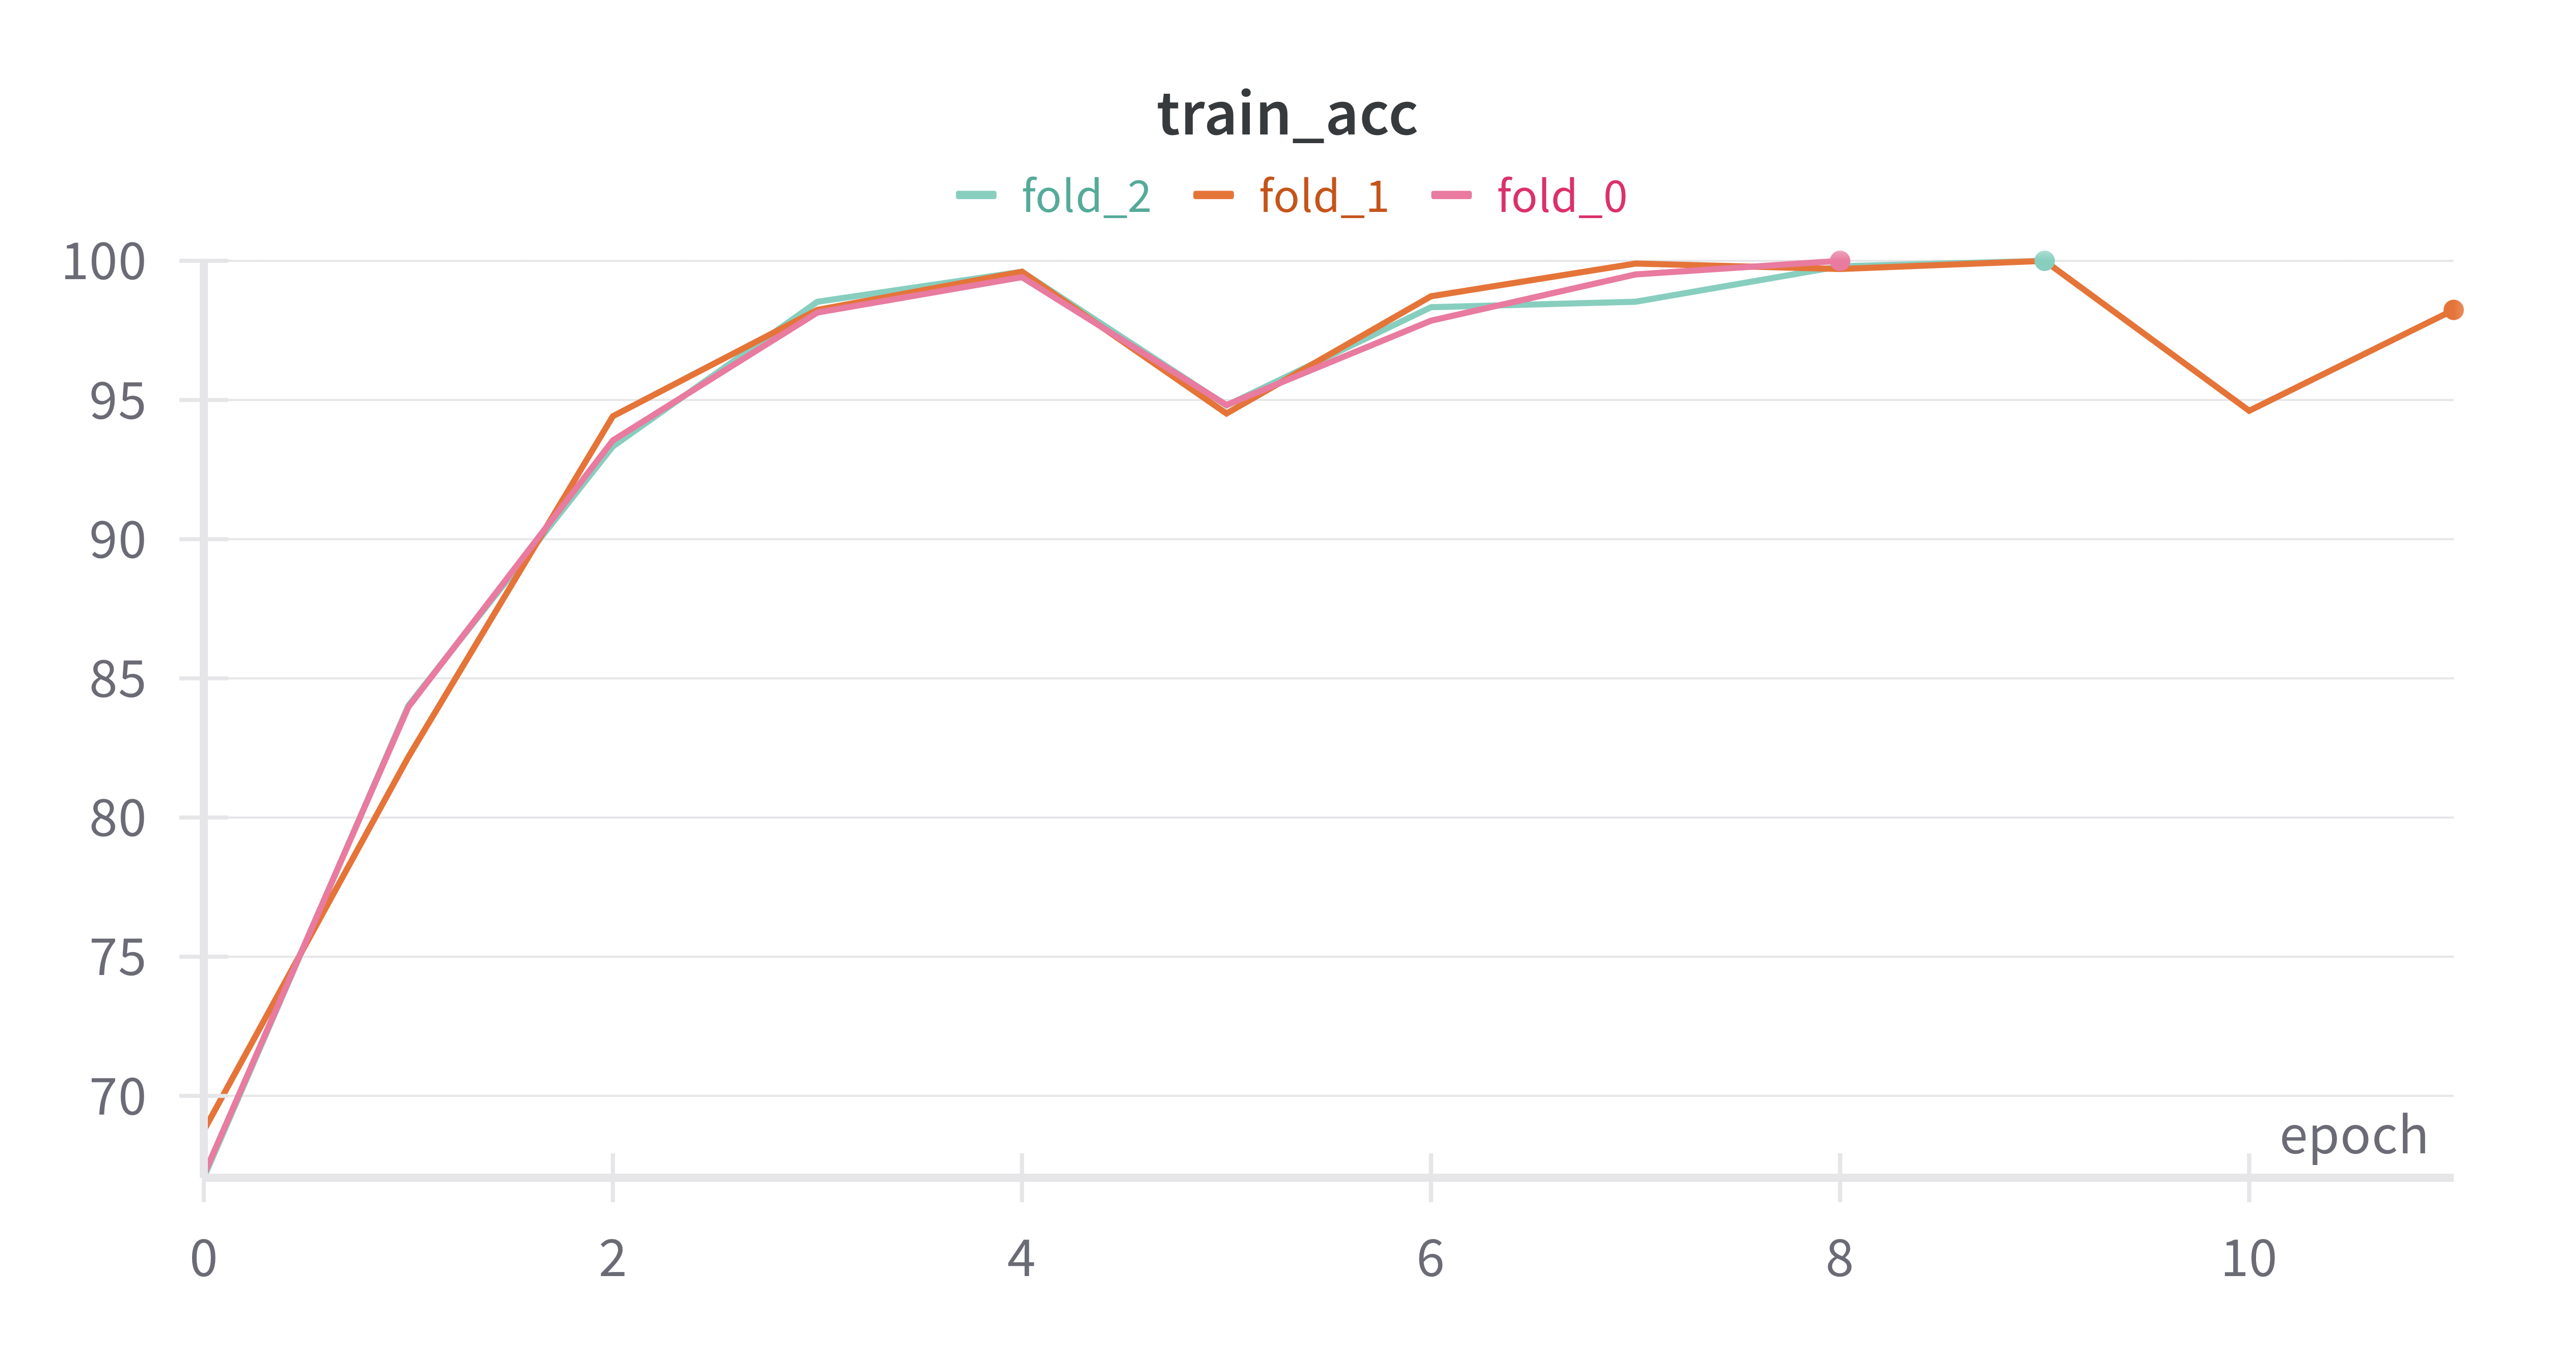
\includegraphics[width=0.6\textwidth]{figures/3f_train_acc.png}
  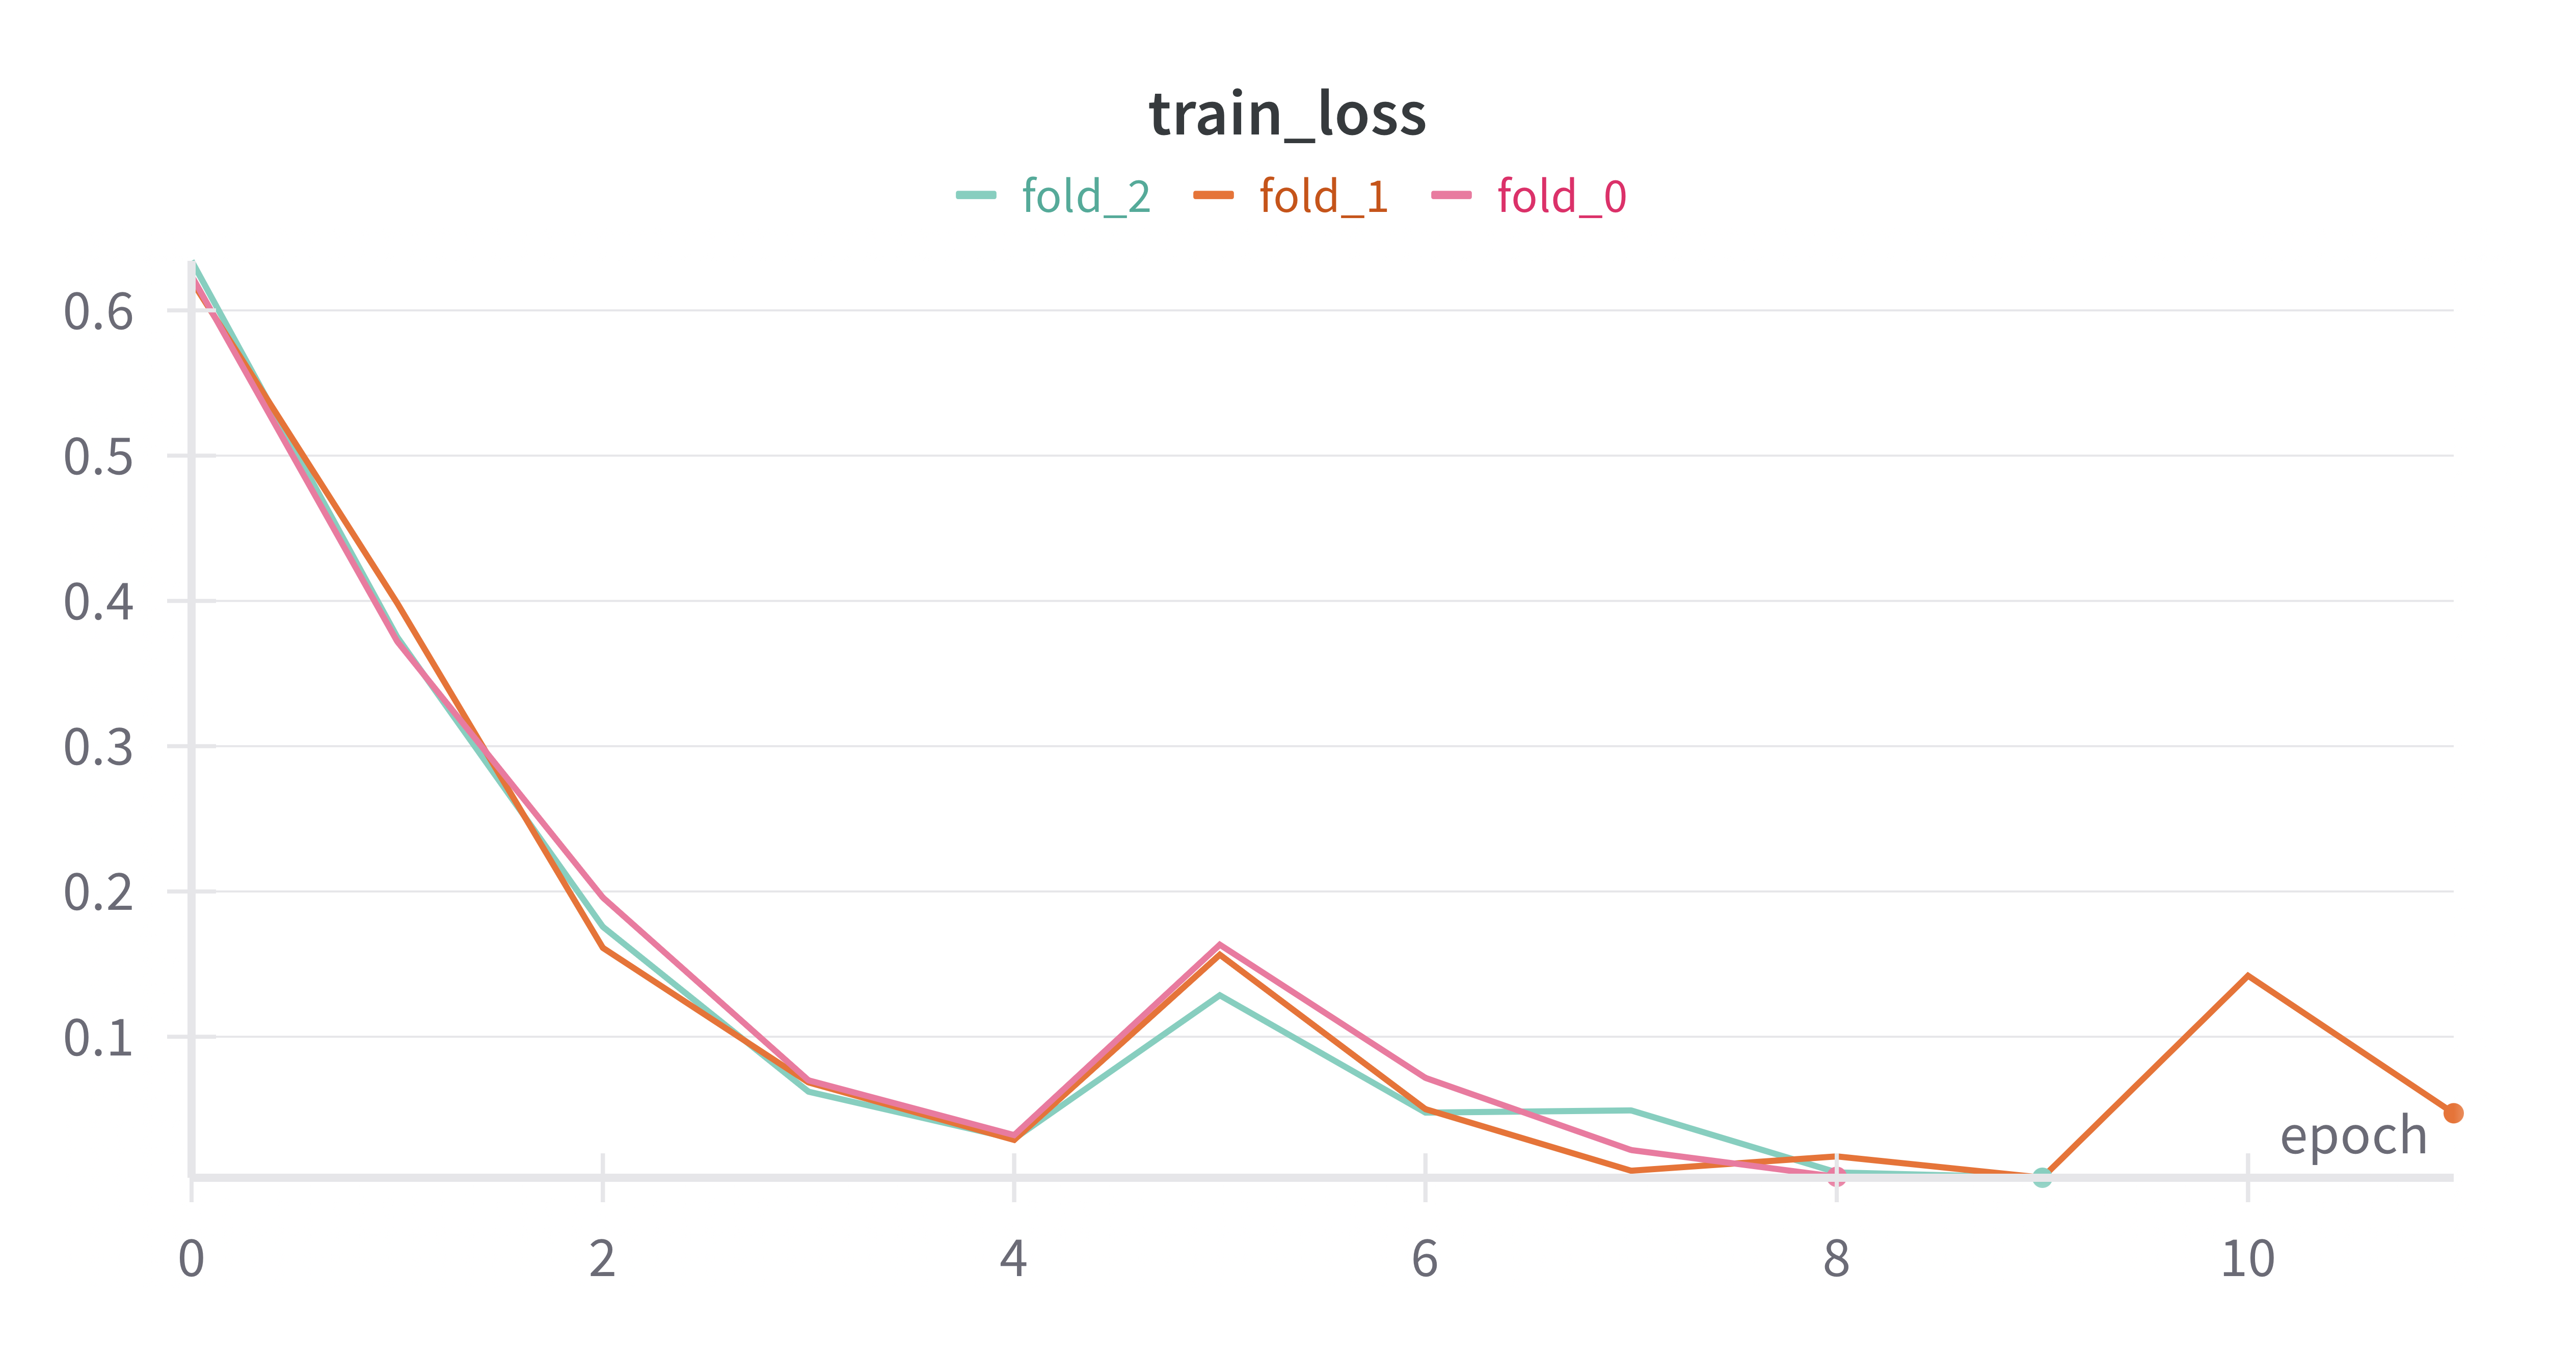
\includegraphics[width=0.6\textwidth]{figures/3f_train_loss.png}
  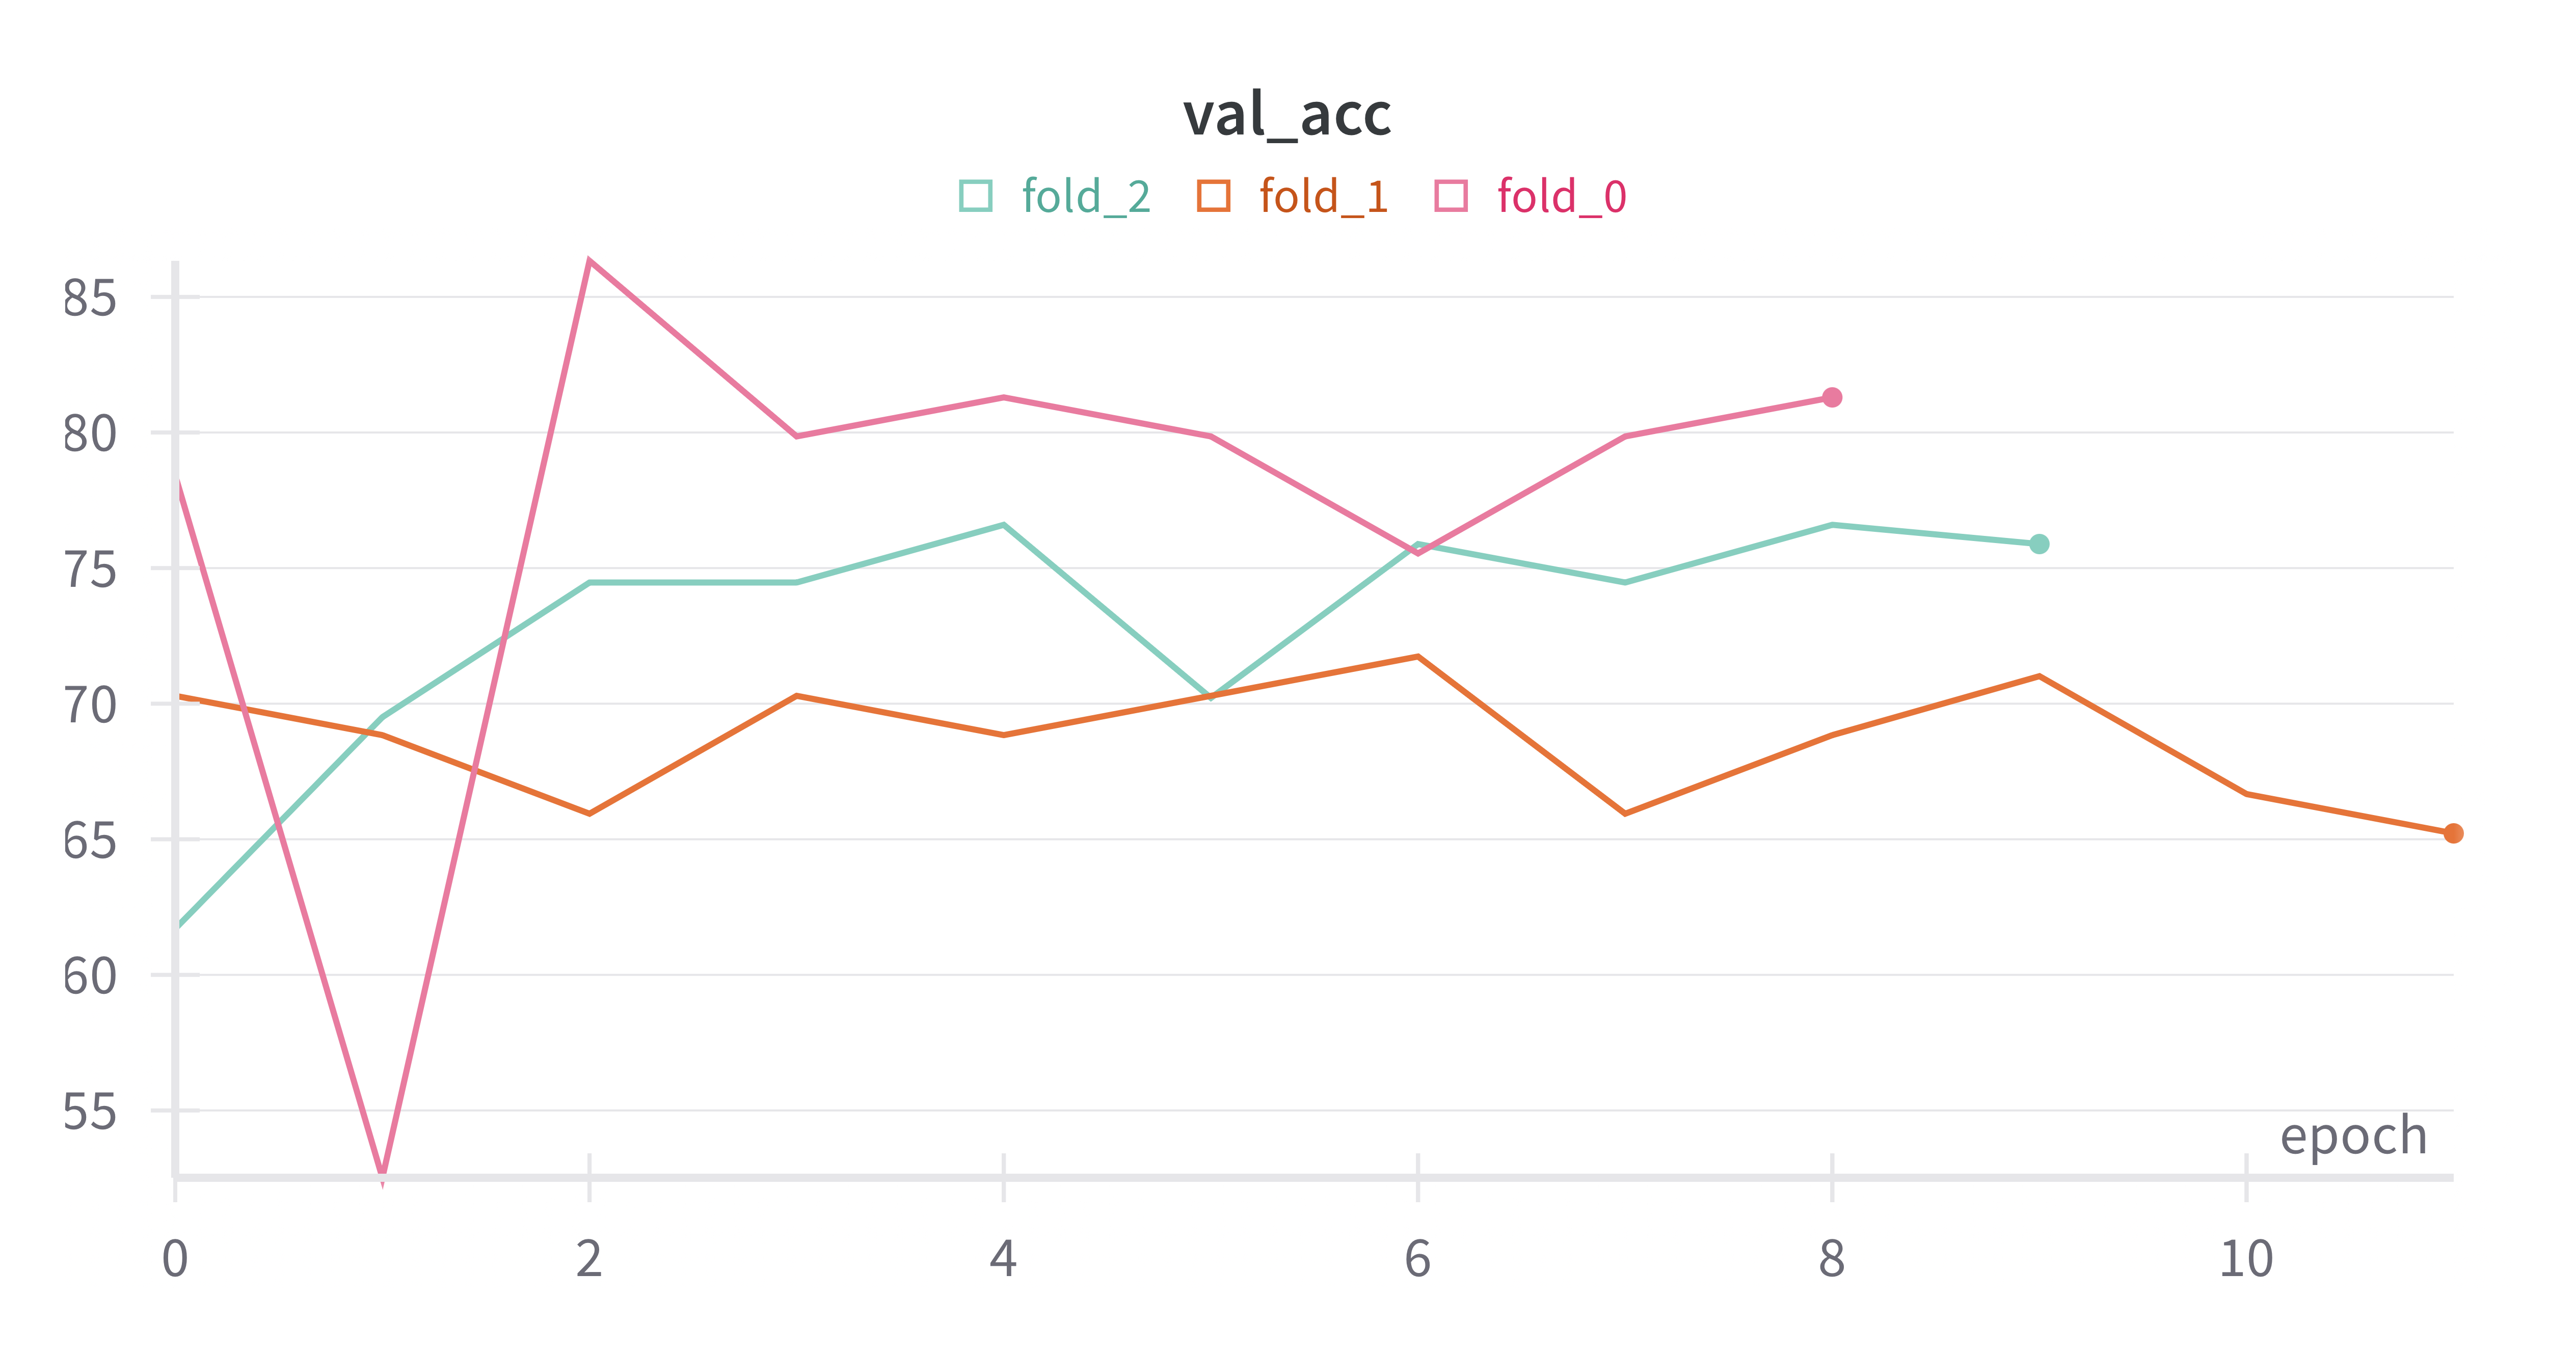
\includegraphics[width=0.6\textwidth]{figures/3f_val_acc.png}
  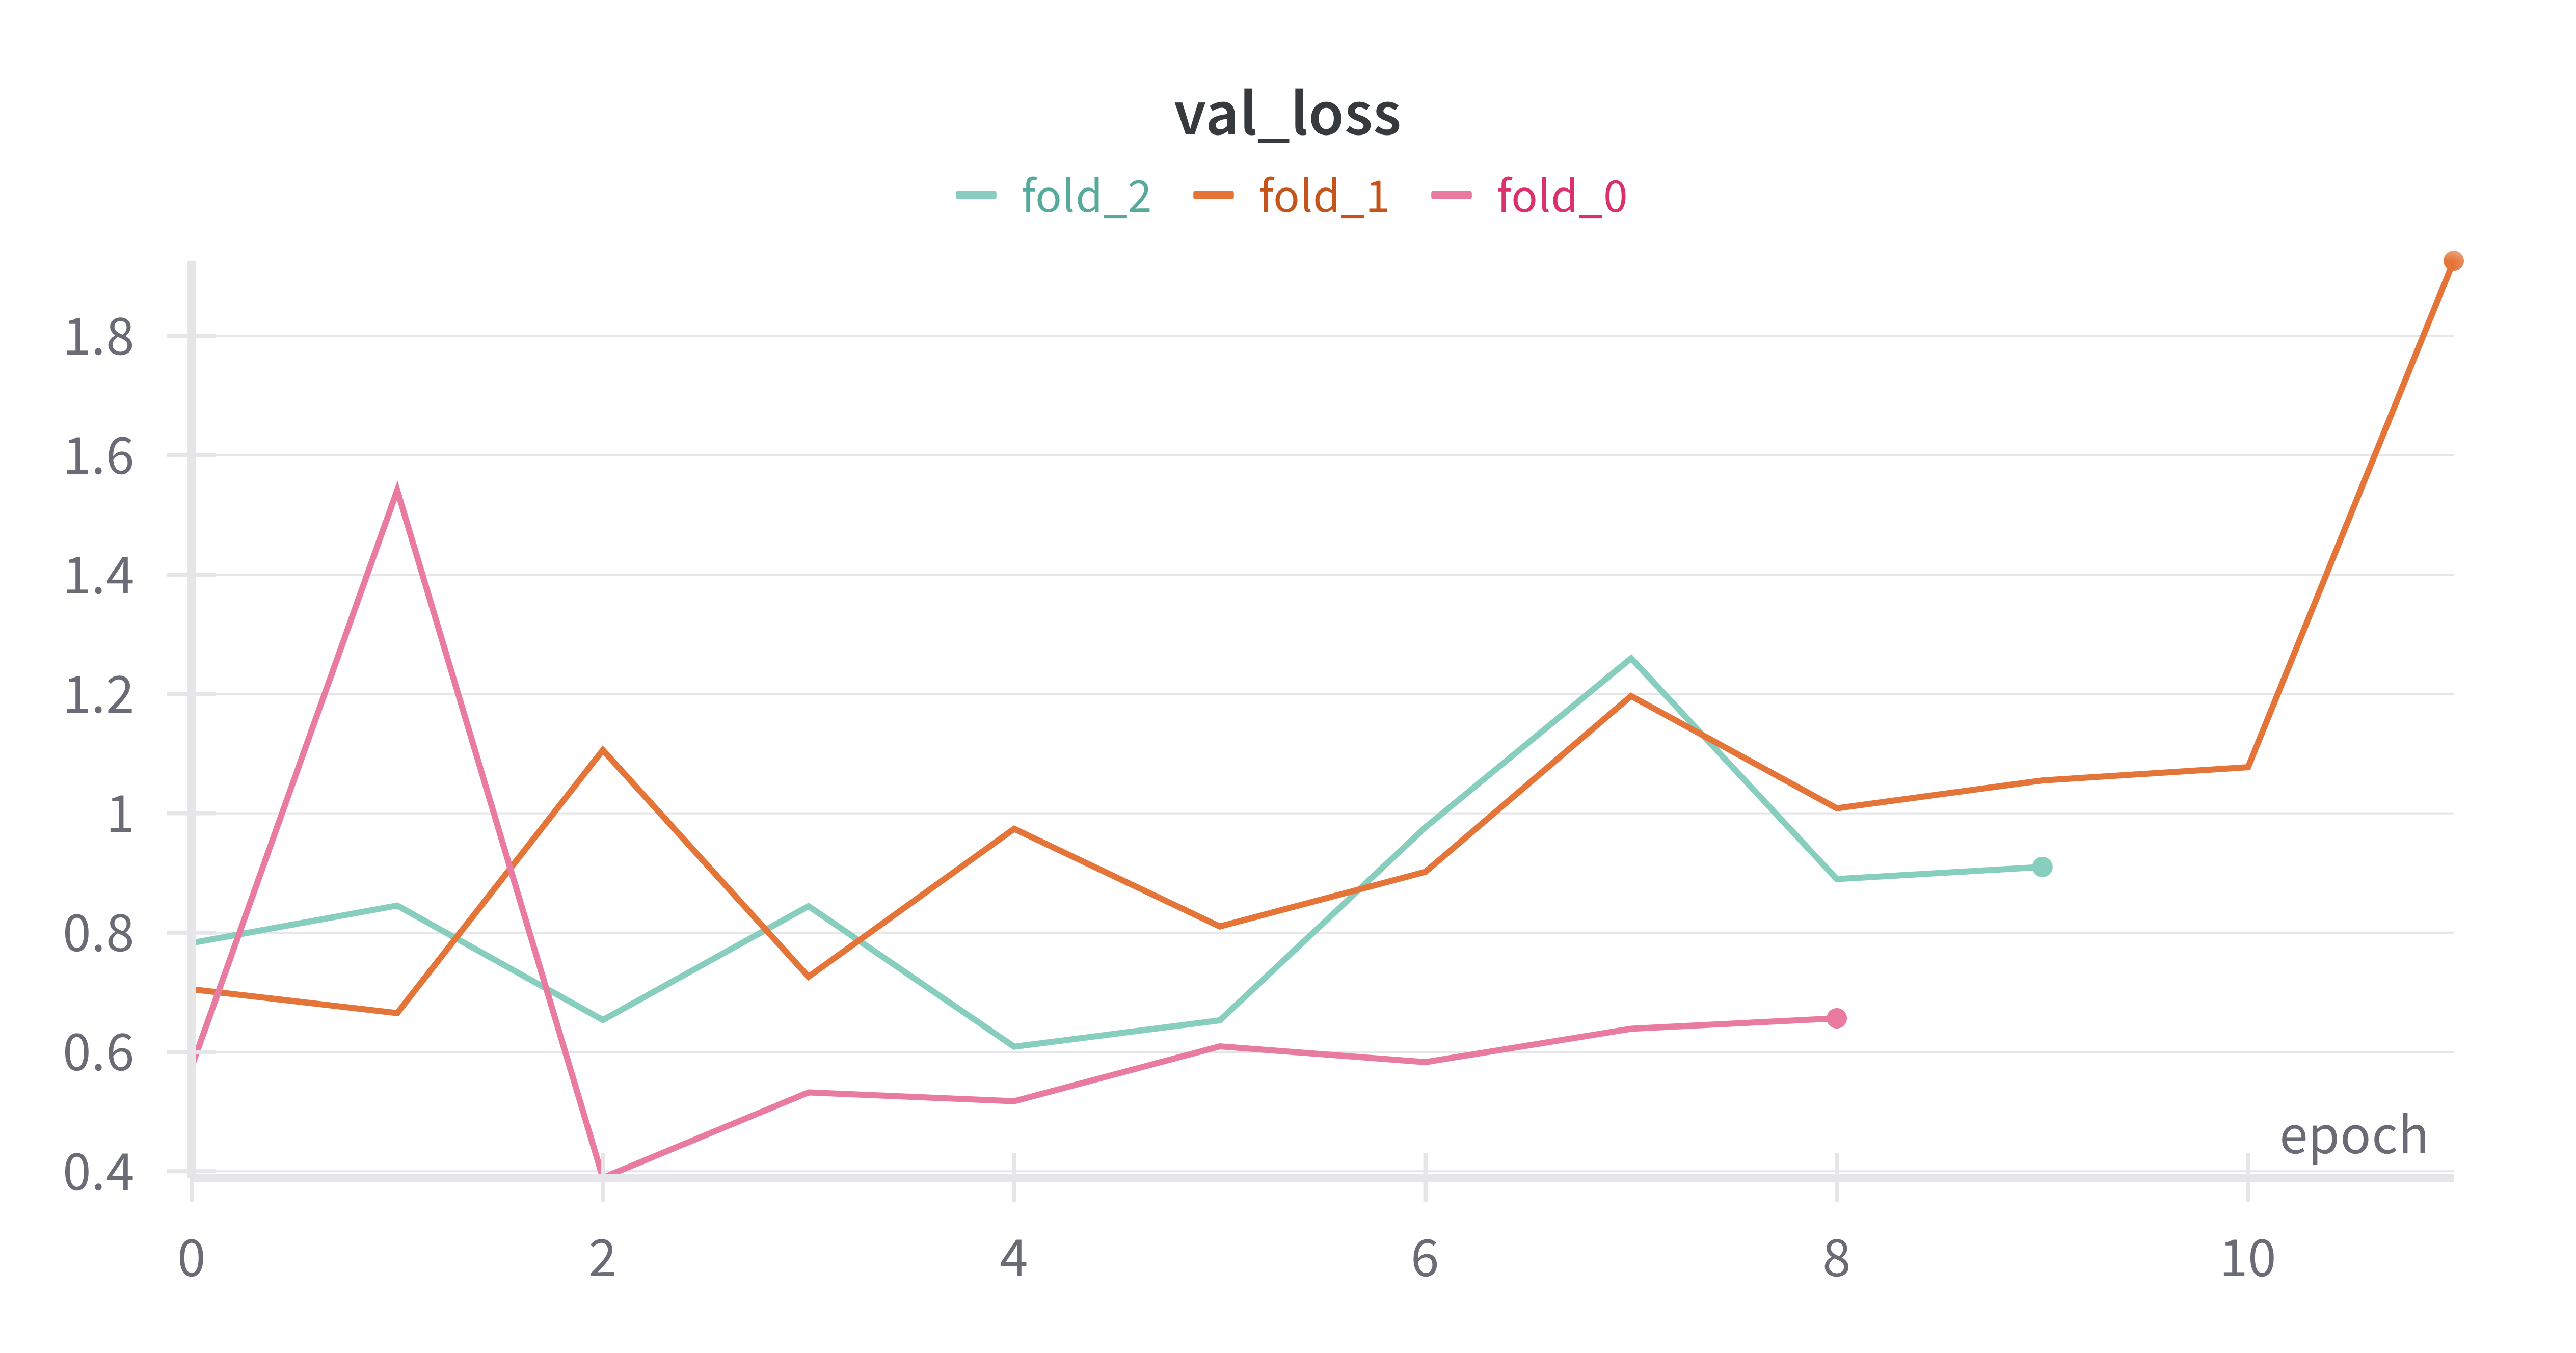
\includegraphics[width=0.6\textwidth]{figures/3f_val_loss.png}
  \caption{Learning curves showing training and validation loss/accuracy across epochs for the R3D-18 model.}
  \label{fig:learning_curves}
\end{figure}

The validation accuracy typically plateaued around epoch 5, after which the early stopping mechanism prevented overfitting by halting training when no further improvement was observed for 5 consecutive epochs.

\subsection{Architectural Insights}

\subsubsection{Dimensional Processing Impact}

A systematic comparison of different 3D architectural variants revealed a clear pattern: performance progressively declined as architectures incorporated more 2D elements. Figure \ref{fig:architecture_comparison_gl} illustrates this comparison across three main architectural approaches.

\begin{figure}[htbp]
  \centering
  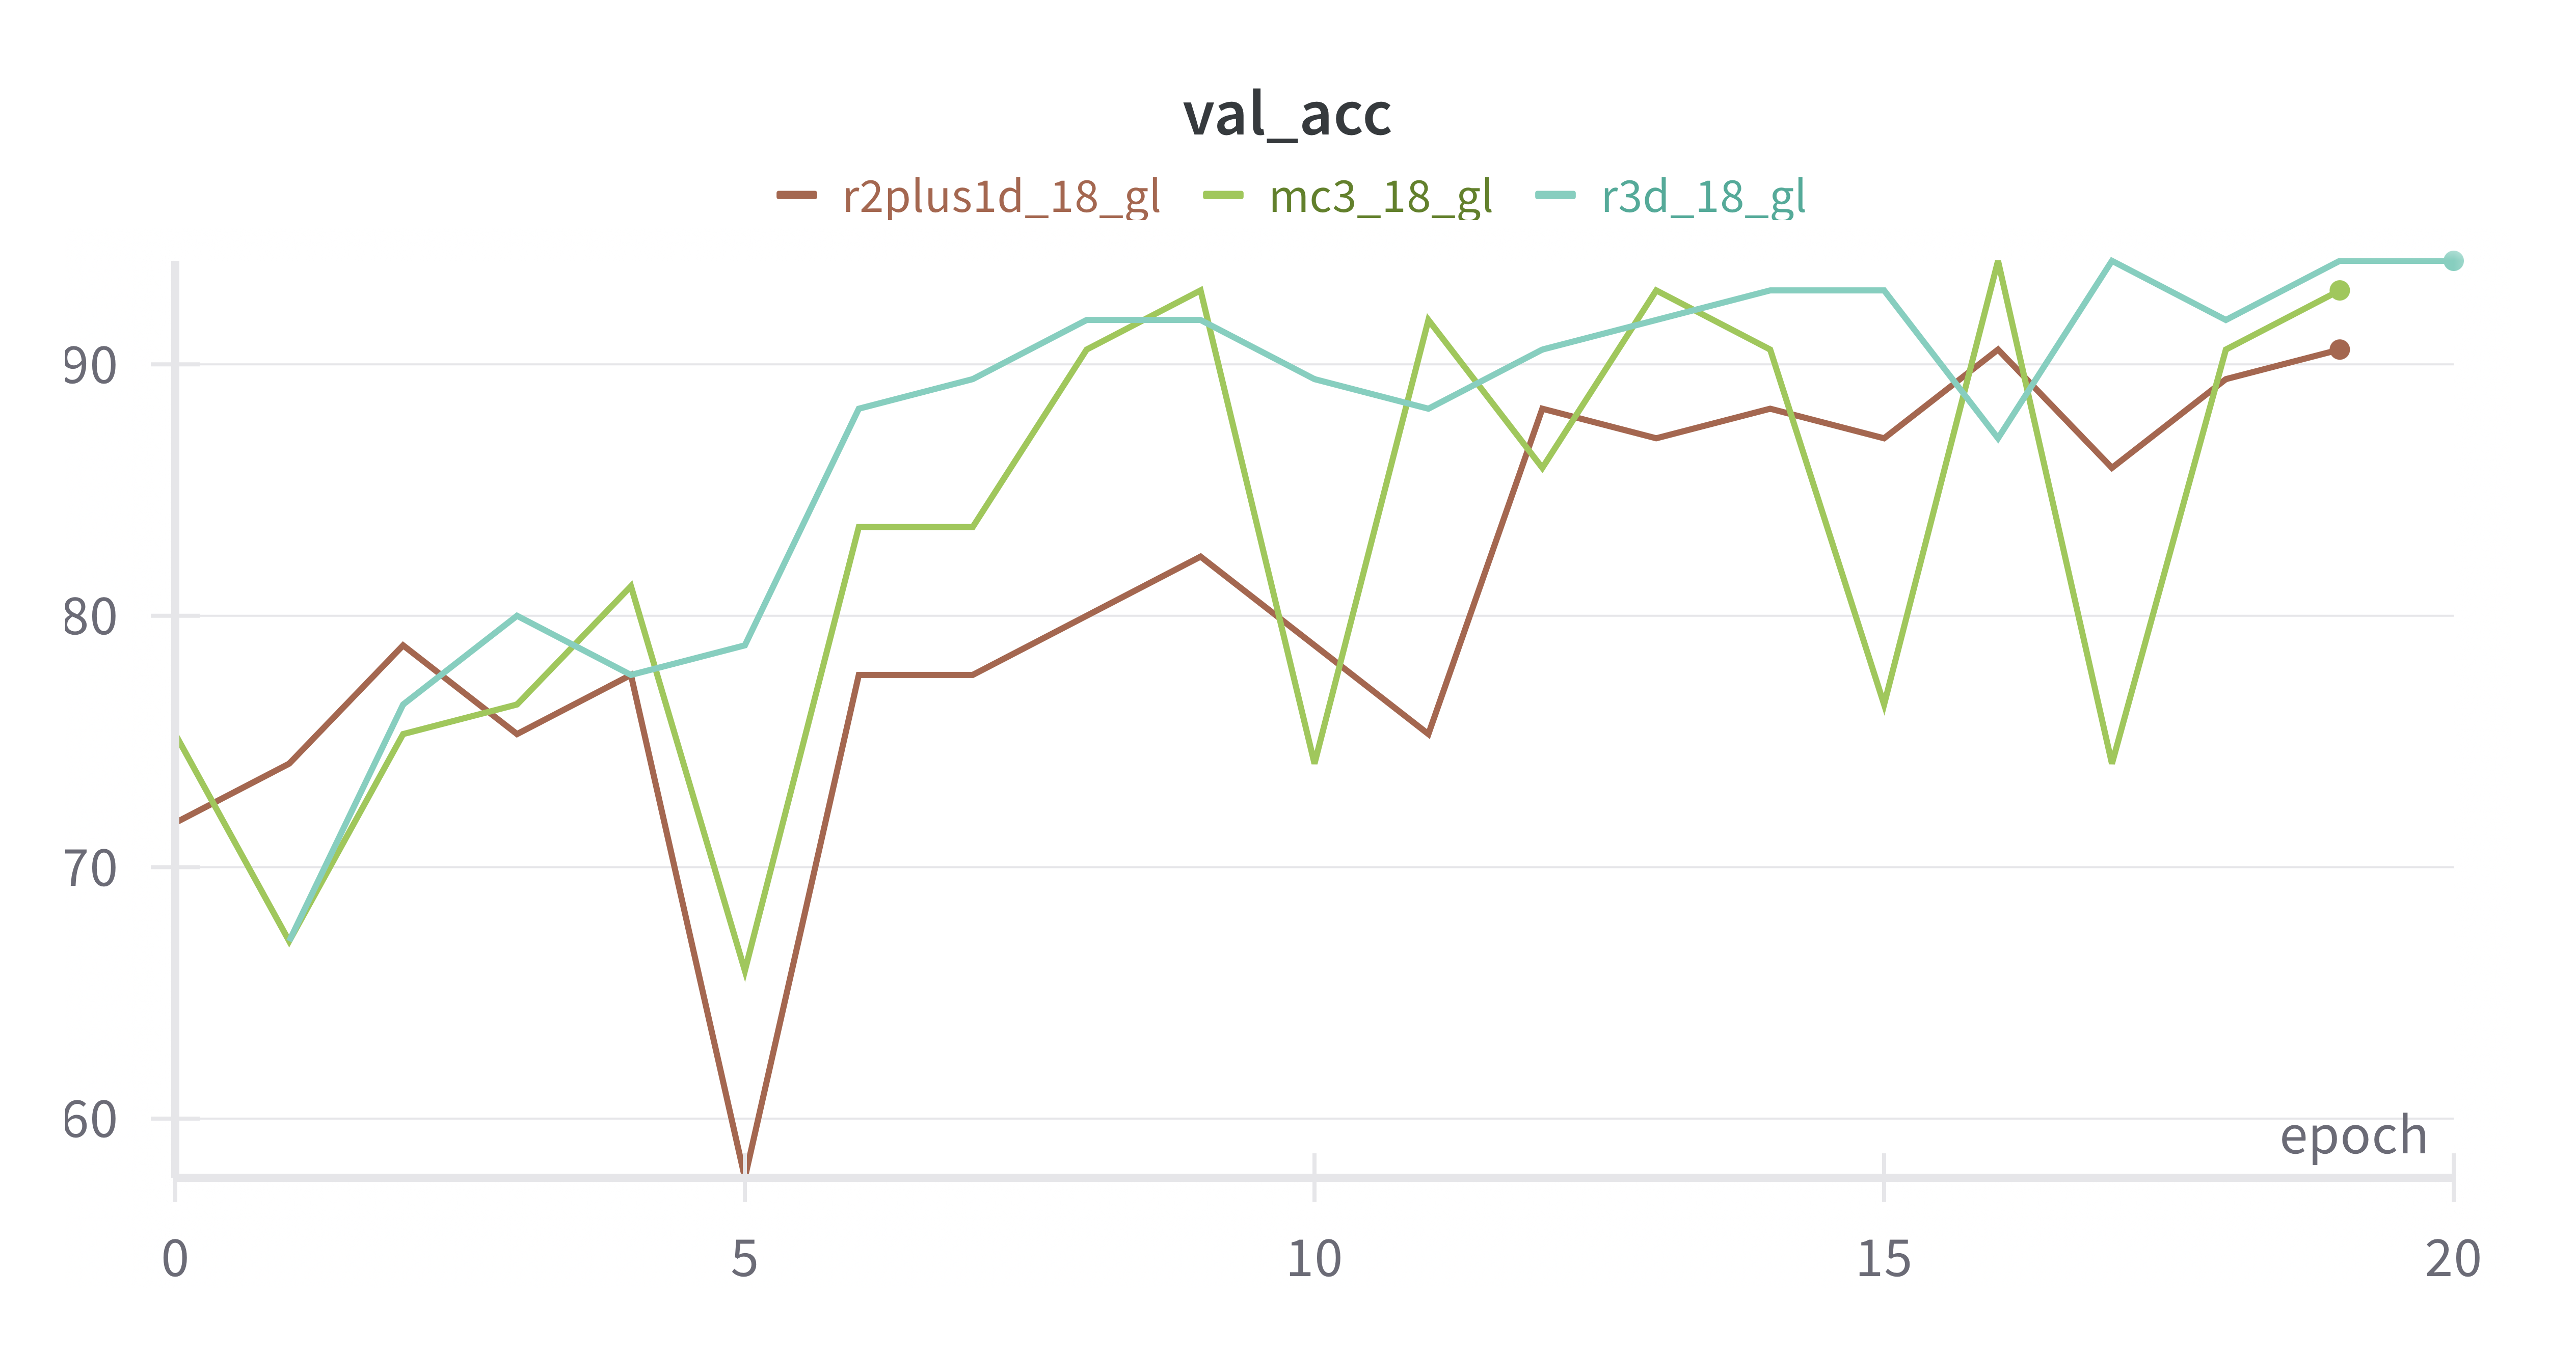
\includegraphics[width=\textwidth]{figures/archs_acc_gl.png}
  \caption{Performance comparison across architectural variants, demonstrating superior performance of fully 3D convolutional approaches (R3D-18) compared to hybrid architectures (MC3-18) and factorized convolutions (R(2+1)D-18). Note, group leakage was present in these runs, leading to inflated scores.}
  \label{fig:architecture_comparison_gl}
\end{figure}

The fully 3D convolutional approach (R3D-18) consistently outperformed both the mixed convolution network (MC3-18) and the factorized convolutional approach (R(2+1)D-18), with test accuracies of 97.67\%, 93.02\%, and 94.18\% respectively; these figures are inflated due to group leakage. This progression strongly suggests that preserving complete 3D spatial context is critical for effective AD classification from volumetric MRI data.

\subsubsection{Layer Freezing Strategy Analysis}

Experiments with different layer freezing strategies revealed significant impact on model stability and performance. Table \ref{tab:freezing_strategies} summarizes these findings.

\begin{table}[htbp]
\centering
\begin{tabular}{|l|c|c|p{4cm}|}
\hline
\textbf{Strategy} & \textbf{Trainable Parameters} & \textbf{Result} & \textbf{Observation} \\
\hline
FC layer only & 0.003\% (1,026) & Failed training & Numerical instability (NaN losses) \\
\hline
FC + Layer 4 & 75.15\% (24.9M) & Successful & Best balance of stability and performance \\
\hline
Full fine-tuning & 100\% (33.1M) & Successful & Increased overfitting risk, slower convergence \\
\hline
\end{tabular}
\caption{Comparison of different layer freezing strategies and their impact on training stability and performance.}
\label{tab:freezing_strategies}
\end{table}
% todo check this cuz it wasn't actually tested from scratch

Notably, attempting to train only the final fully connected layer (preserving 99.997\% of pre-trained weights) resulted in numerical instability, suggesting that significant domain adaptation is necessary for the substantial shift from video action recognition to MRI classification. The optimal approach (FC + Layer 4) balanced stable training with effective knowledge transfer.

\subsubsection{Computational Performance Analysis}

Training on a consumer-grade M1 Mac using Metal Performance Shaders demonstrated both the feasibility and challenges of developing deep learning models for neuroimaging on accessible hardware. Table \ref{tab:computational_performance} summarizes the computational characteristics of different architectures.

\begin{table}[htbp]
\centering
\begin{tabular}{|l|c|c|c|}
\hline
\textbf{Architecture} & \textbf{Training Time/Epoch} & \textbf{Memory Usage} \\
\hline
R3D-18 & $\sim$1 hour & 7.5 GB \\
\hline
MC3-18 & $\sim$4 hours & 7.6 GB \\
\hline
R(2+1)D-18 & $\sim$5 hours & 7.4 GB \\
\hline
MViT & Failed (OOM) & >32 GB (estimated) \\
\hline
\end{tabular}
\caption{Computational performance metrics for different model architectures.}
\label{tab:computational_performance}
\end{table}

Despite optimization attempts (mixed precision, layer optimization, batch size tuning), the forward pass remained the primary bottleneck in the training process. The memory constraints also prevented exploration of larger transformer-based architectures like MViT, which required an estimated >32GB of memory for the 128³ input volumes.

\subsection{Preprocessing Impact Analysis}

\subsubsection{Resolution and Cropping Strategy Evaluation}

The adaptive cropping strategy yielded substantial performance improvements compared to naive interpolation. As shown in Figure \ref{fig:cropping_impact}, the accuracy differential between models trained on 96³ naively interpolated volumes versus 128³ adaptively cropped volumes was significant.

\begin{figure}[htbp]
  \centering
  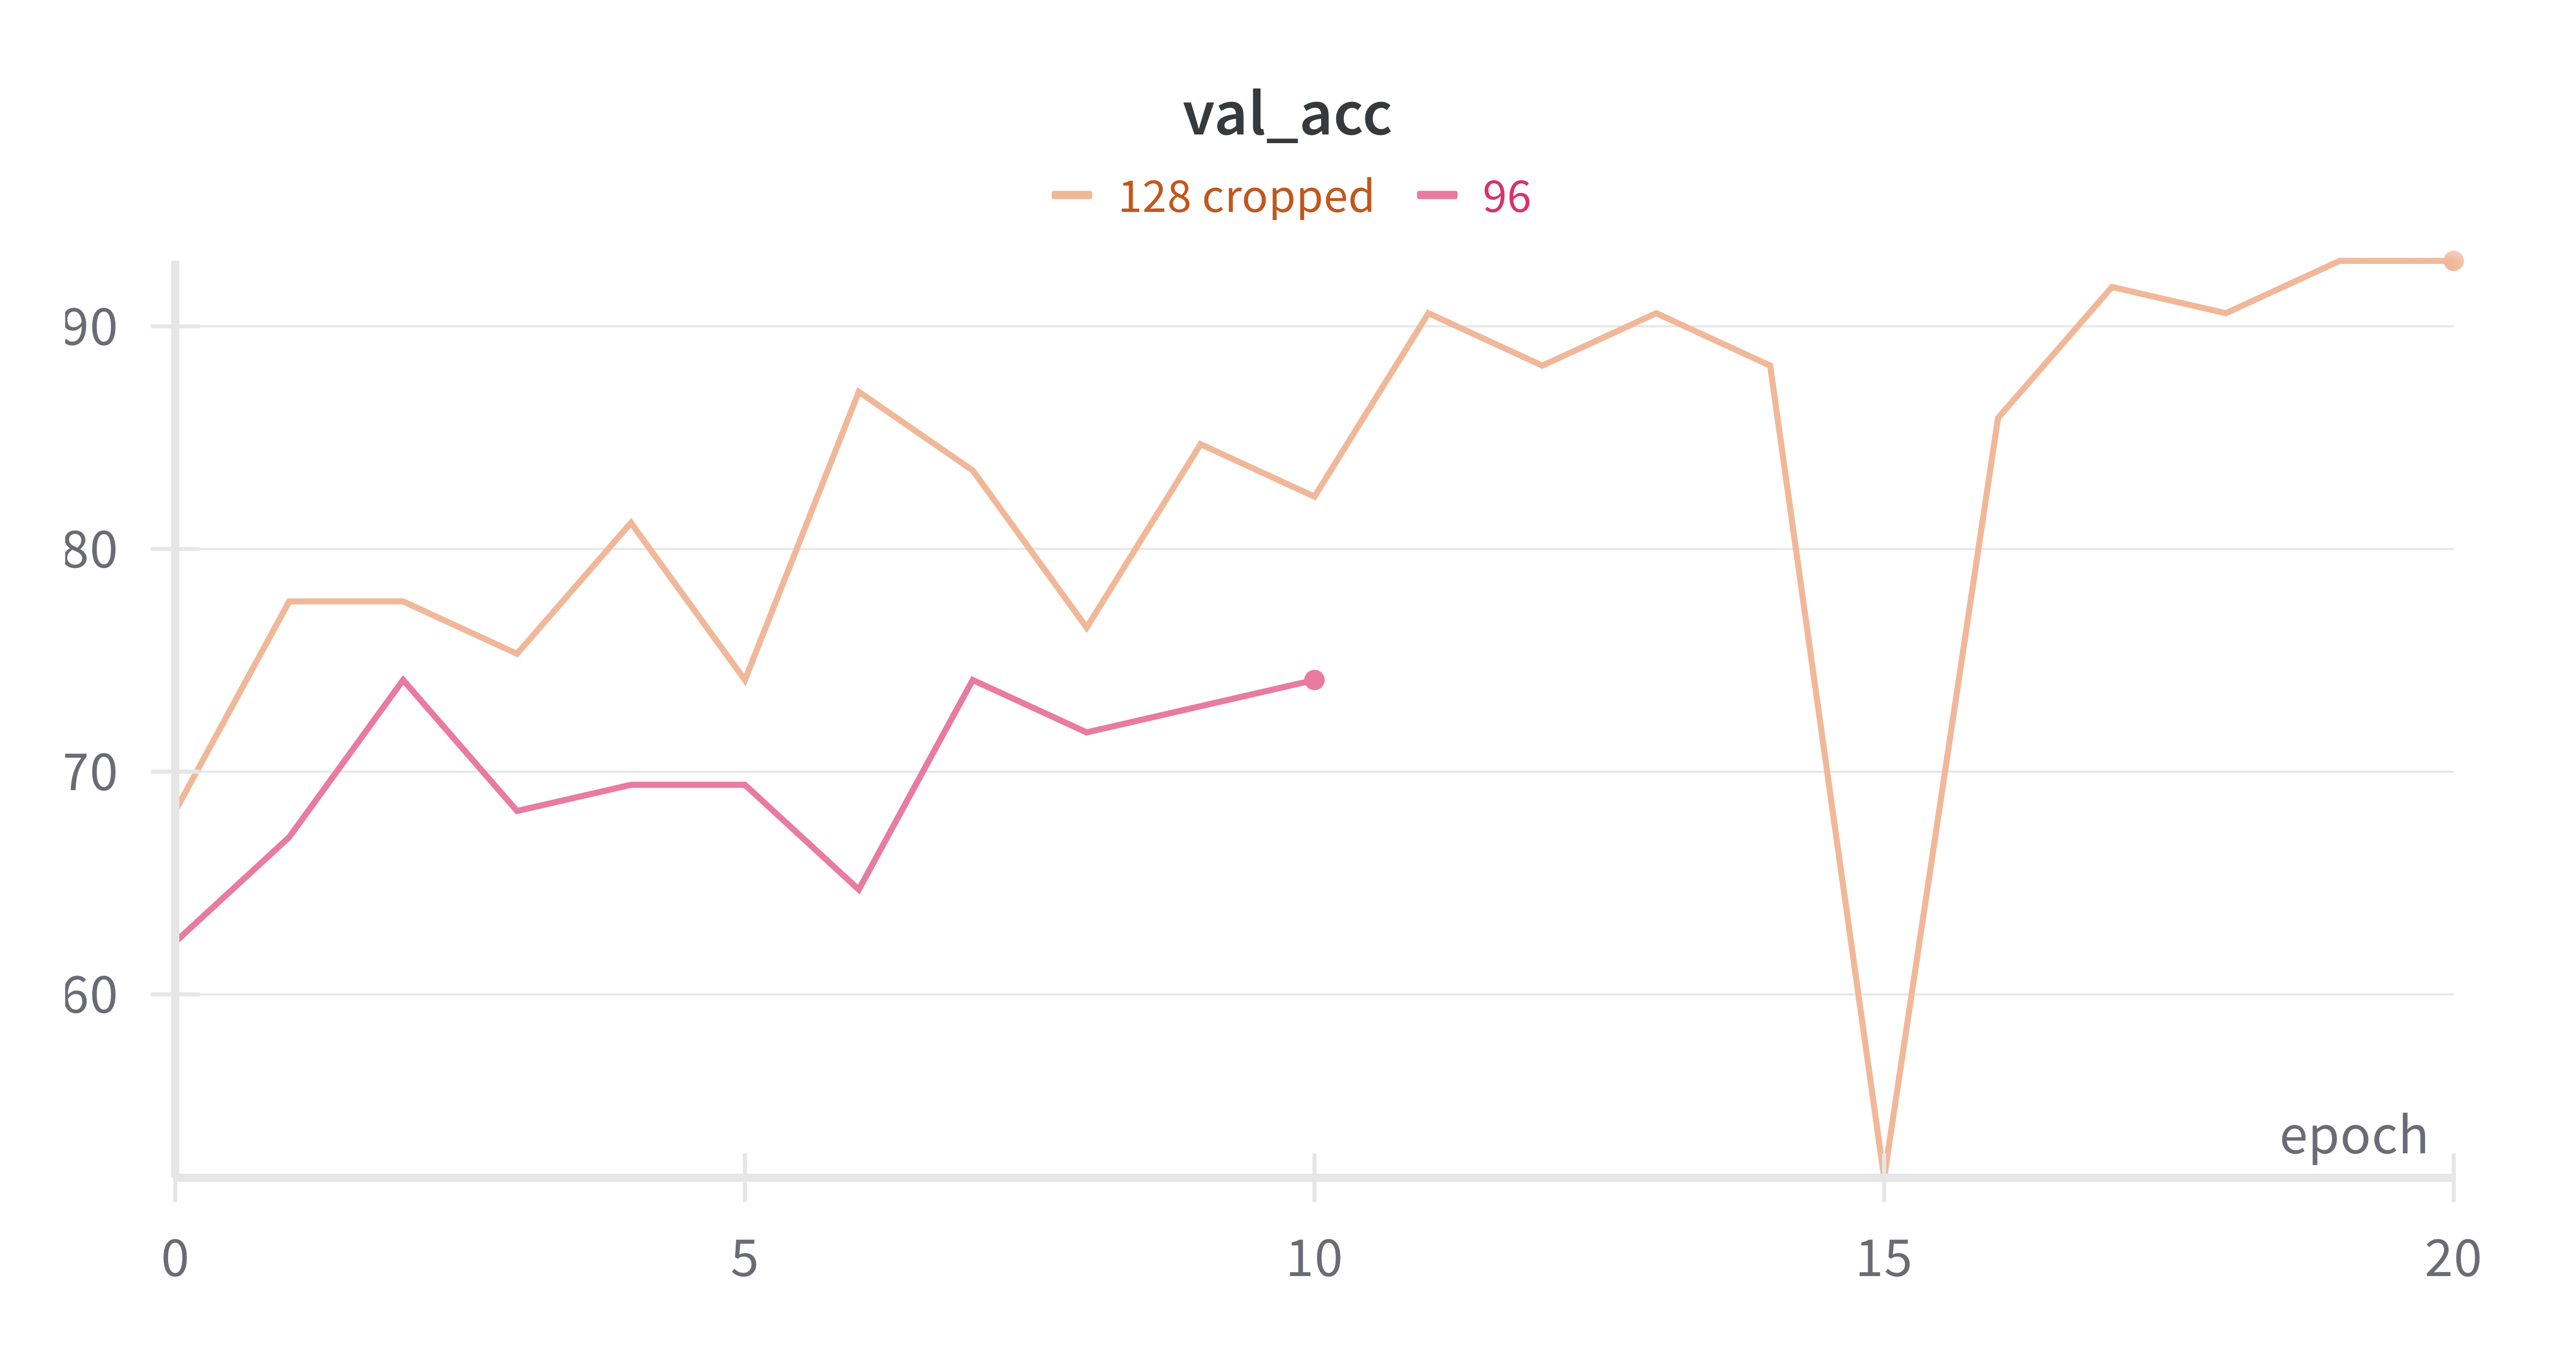
\includegraphics[width=0.8\textwidth]{figures/crop_val_acc.png}
  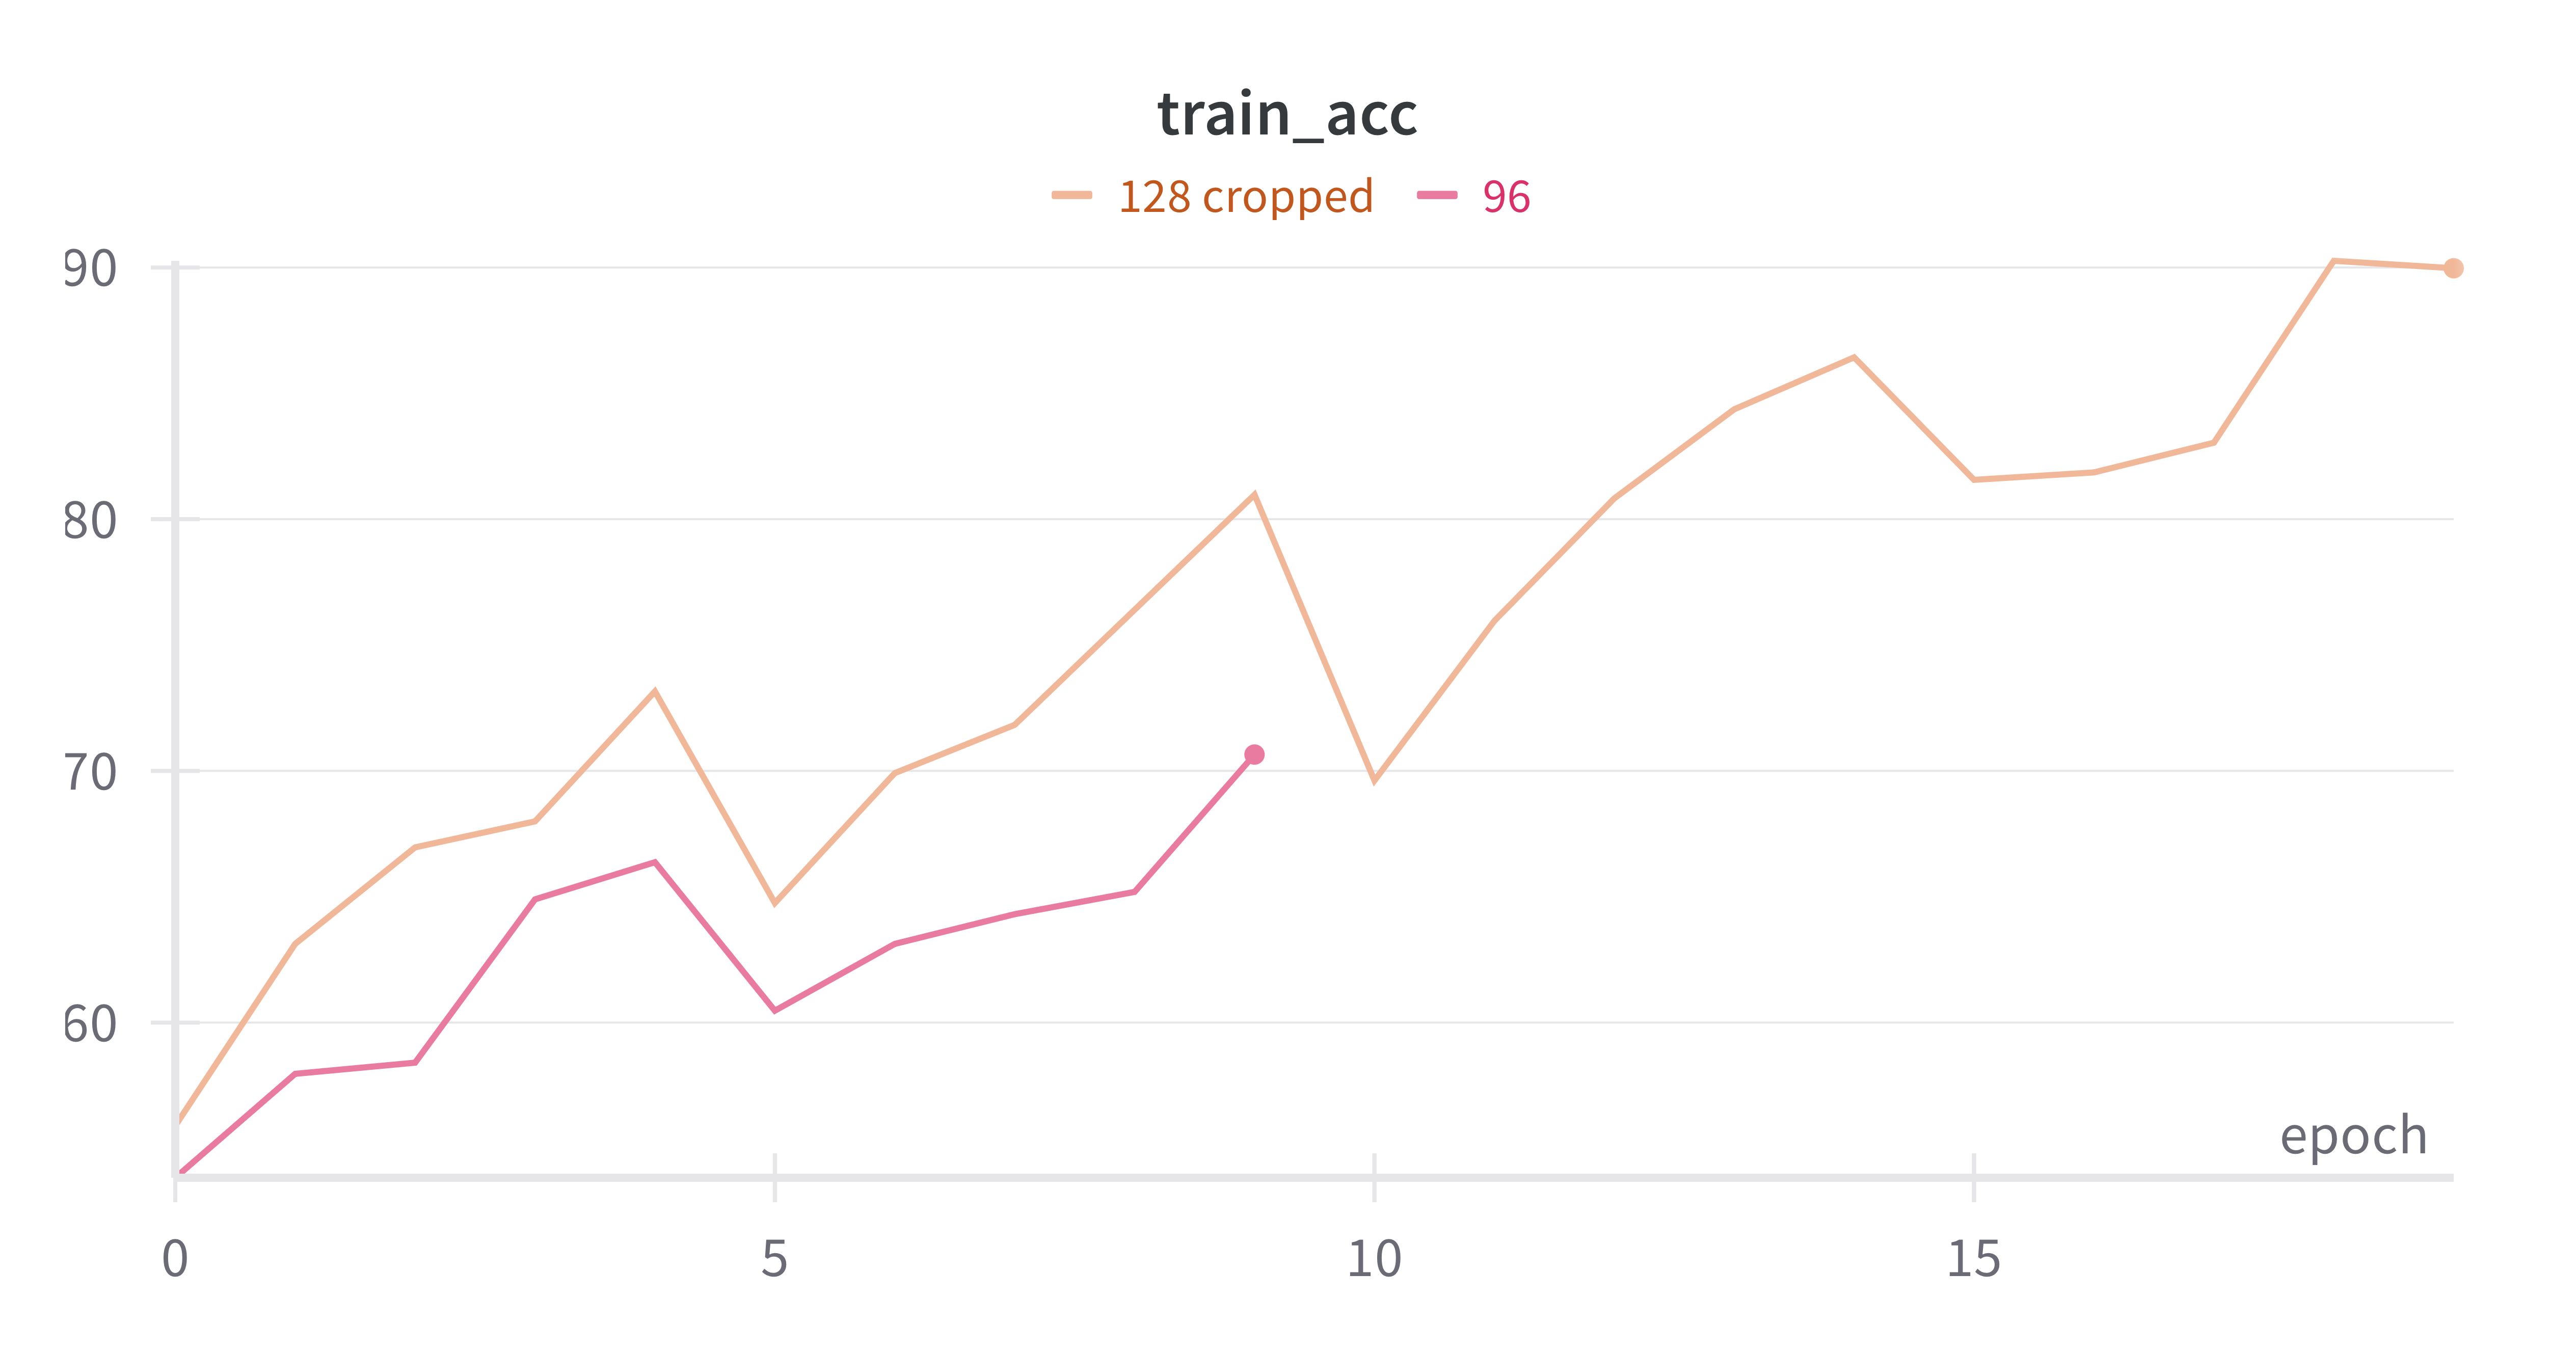
\includegraphics[width=0.8\textwidth]{figures/crop_train_acc.png}
  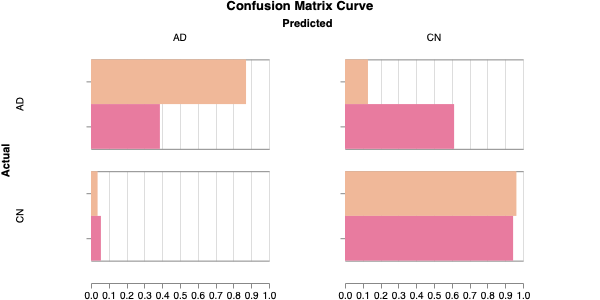
\includegraphics[width=0.8\textwidth]{figures/crop_CM.png}
  \caption{Performance comparison between naive downsampling (96³) and adaptive cropping with higher resolution (128³), demonstrating the importance of preserving anatomical detail. Note: This inflated accuracy is due to group leakage having not yet been implemented, but all else is equal despite the 96³ vs 128³ difference.}
  \label{fig:cropping_impact}
\end{figure}

This improvement can be attributed to the preservation of $\sim$35\% more effective resolution for critical structures like the hippocampu as well as a 2.37x increase in resolution, allowing the model to better detect subtle atrophy patterns characteristic of AD.

\subsubsection{Skull Stripping Quality}

SynthStrip was selected as the skull stripping method for all preprocessing due to its known advantages in handling atrophied brains. While a direct comparison between skull stripping methods was not performed, qualitative assessment of the SynthStrip results showed excellent preservation of cortical boundaries and consistent handling of atrophied brain regions characteristic of Alzheimer's disease. Figure \ref{fig:skull_stripping_comparison} shows example outputs from SynthStrip, demonstrating its effectiveness across different subjects in the dataset.

The literature suggests that high-quality skull stripping is important for AD classification tasks, with previous studies reporting performance differences of 2-4\% between optimal and suboptimal brain extraction methods \cite{hoopes2022synthstrip}. By employing SynthStrip consistently across all scans, non-brain tissue did not introduce confounding signals that might otherwise impact the model's ability to identify disease-specific patterns.

\begin{figure}[htbp]
  \centering
  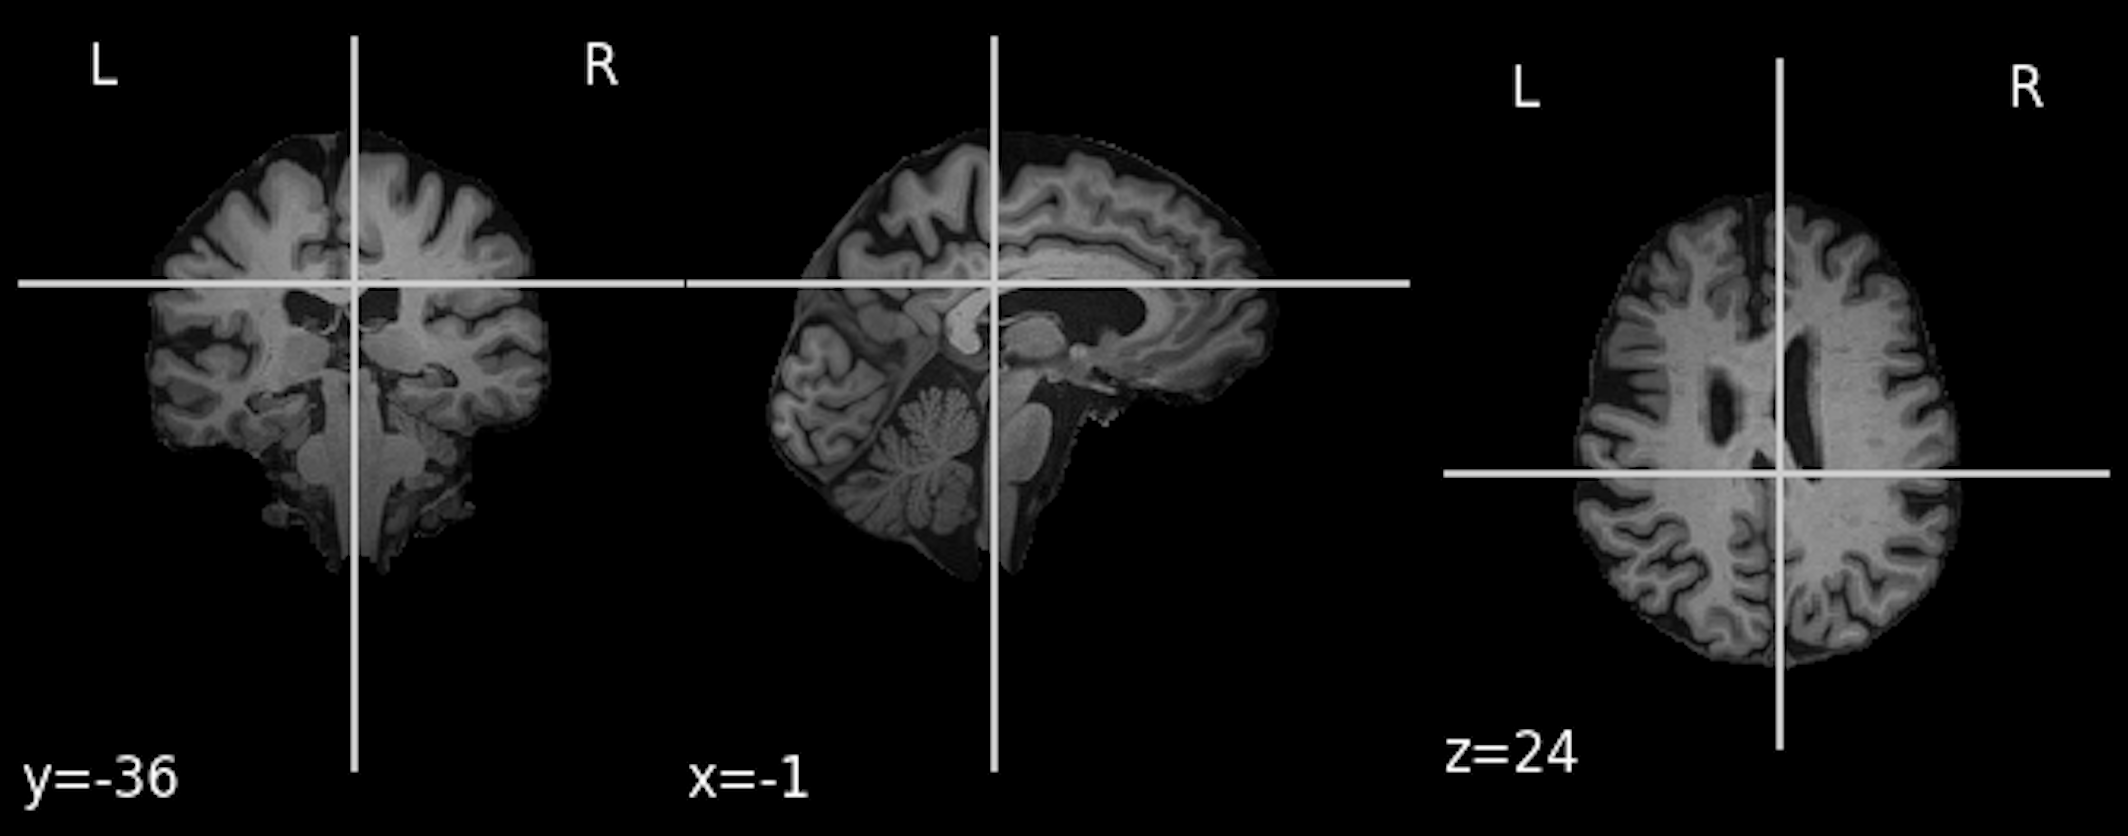
\includegraphics[width=\textwidth]{figures/ss.png}
  \caption{Example SynthStrip output.}
  \label{fig:skull_stripping_comparison}
\end{figure}

\subsubsection{Augmentation and Normalization Effects}

Through systematic experimentation, it was identified that minimal, targeted augmentation outperformed more extensive transformation sets. Figure \ref{fig:augmentation_comparison} illustrates the performance impact of different augmentation strategies. $tio_s$ and $tio_l$ being torchio augmentations with smaller and larger values, the augmentations include rotations, translations, random noise, gamma adjustment, and z-normalization, showing the effectiveness of minimalist approach focusing on noise, gamma adjustment, and normalization versus more extensive transformations. $tio_flip$ was $tio_s$ plus flips, and $monai$ was using similar augmentations to $tio_flip$ but using the monai library.

\begin{figure}[htbp]
  \centering
  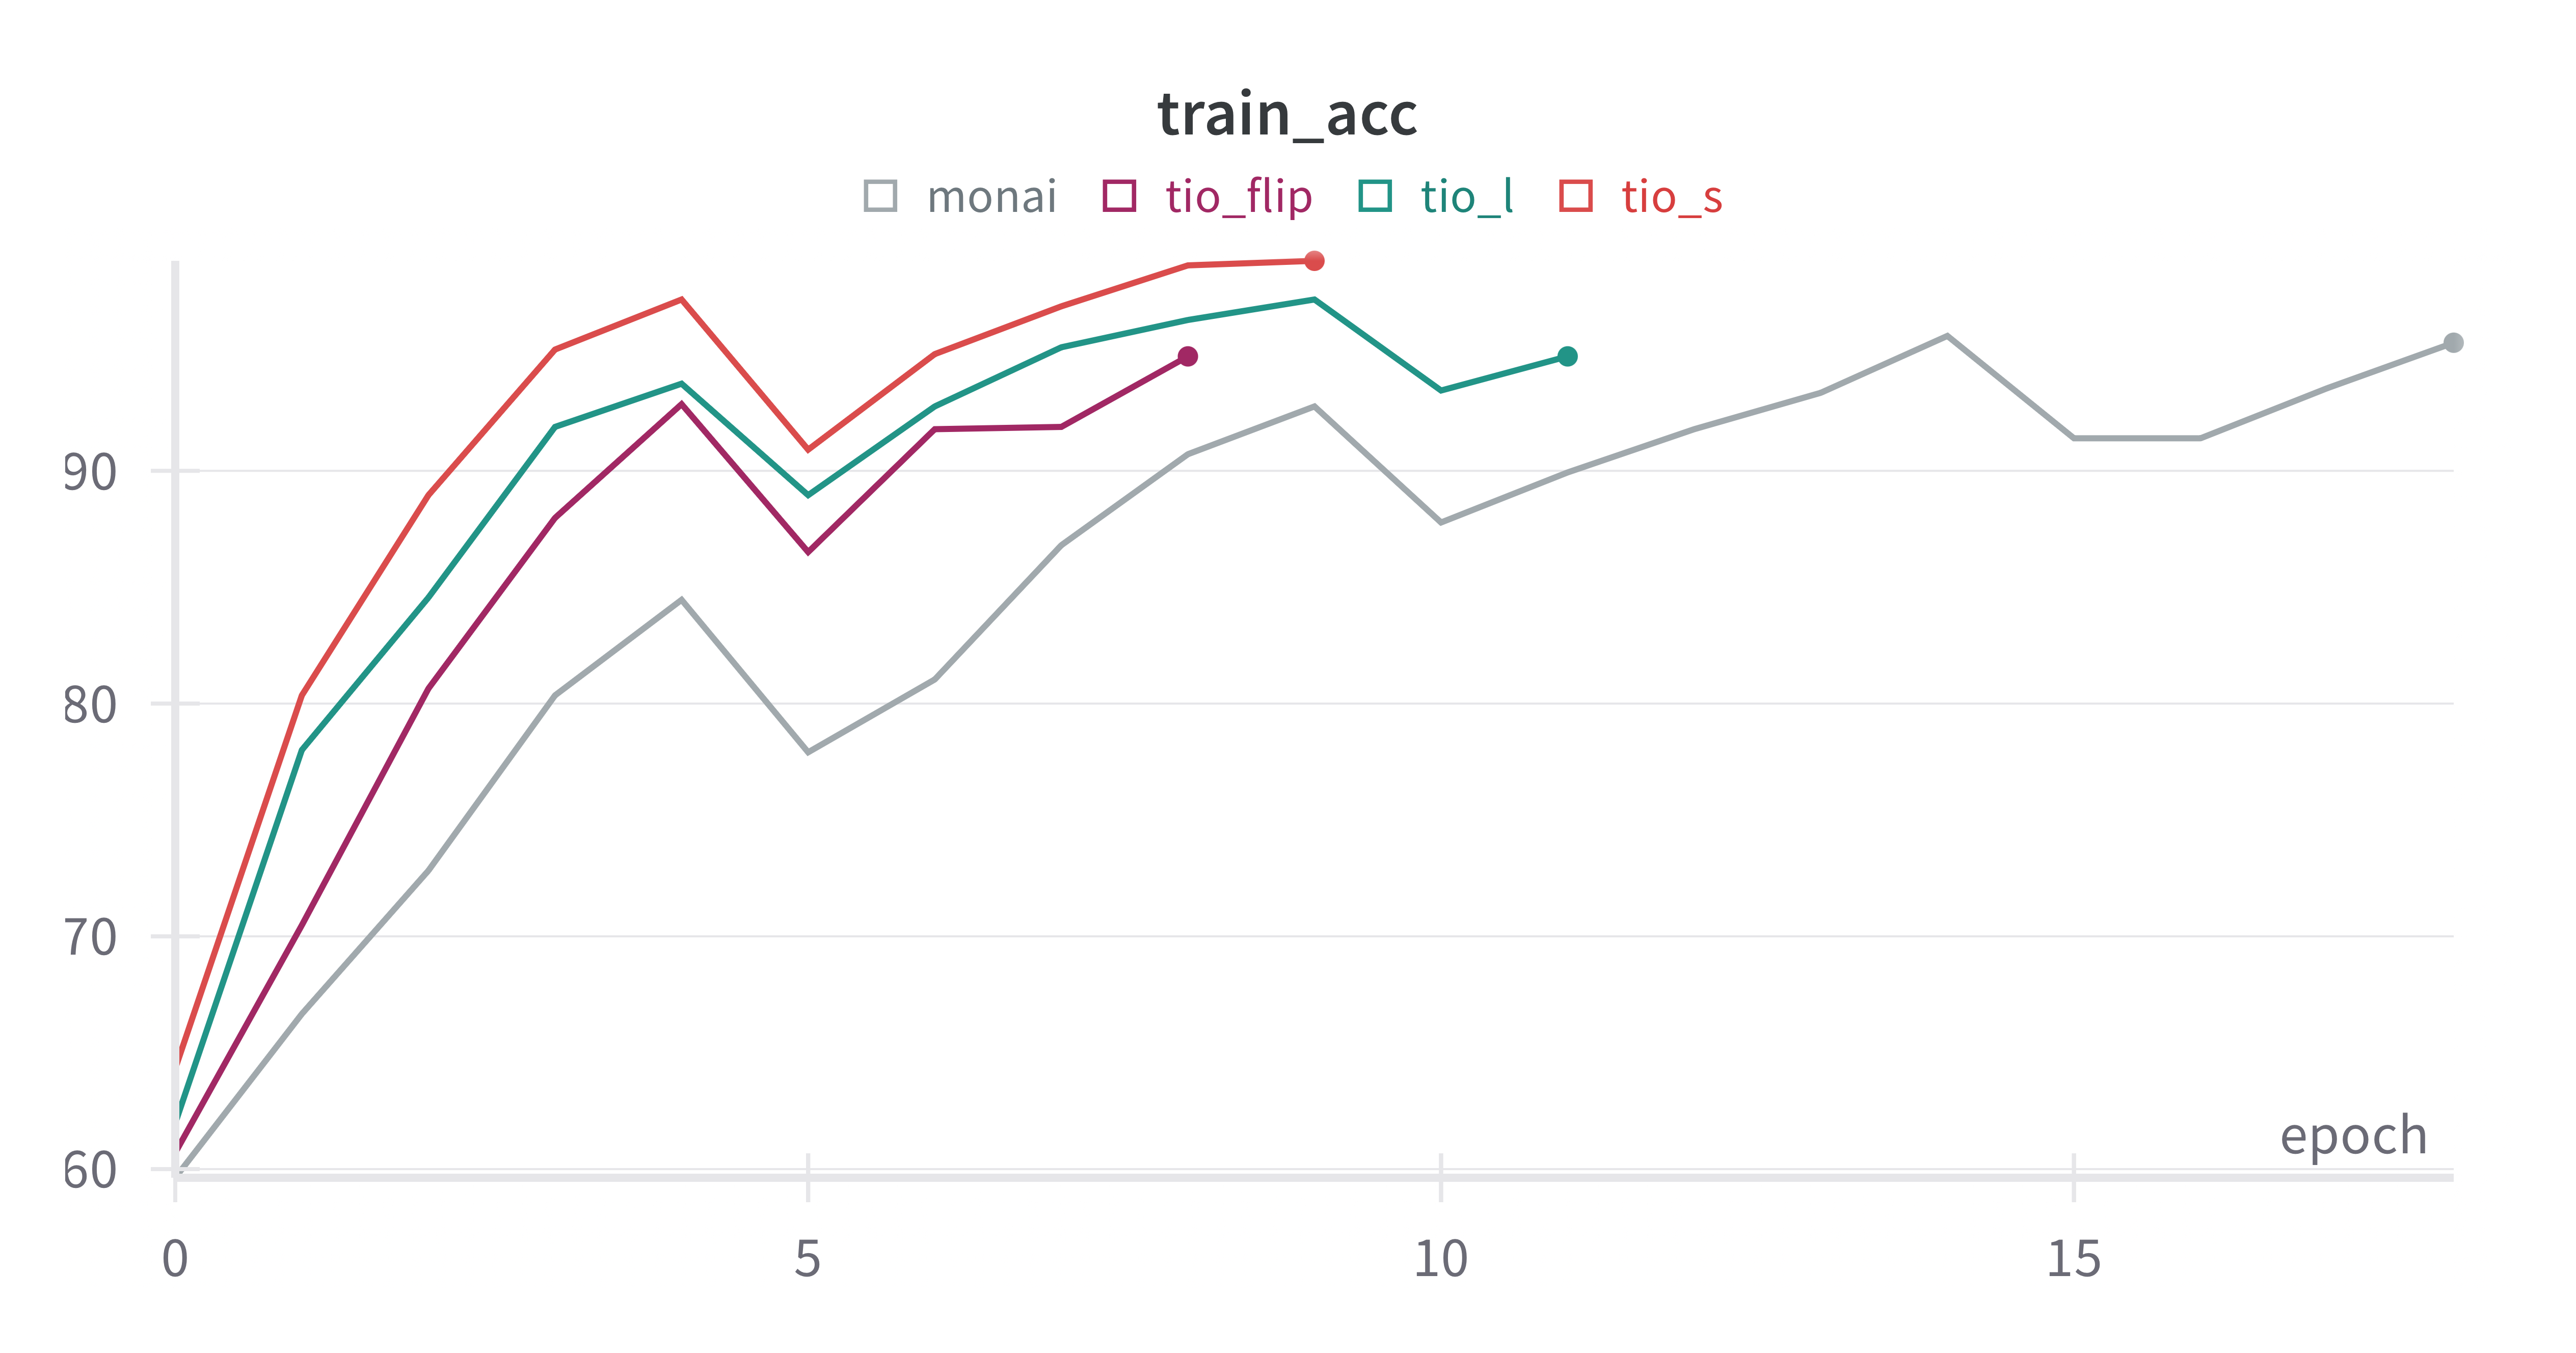
\includegraphics[width=\textwidth]{figures/augs_train_acc.png}
  \caption{Training accuracy performance comparison across different augmentation strategies.}
  \label{fig:augmentation_comparison}
\end{figure}

Z-normalization proved particularly effective, as demonstrated in Figure \ref{fig:normalisation_accuracy} which shows the consistent improvement in validation accuracy as well as a more stable convergence when normalization was included in the augmentation pipeline.

\begin{figure}[htbp]
  \centering
  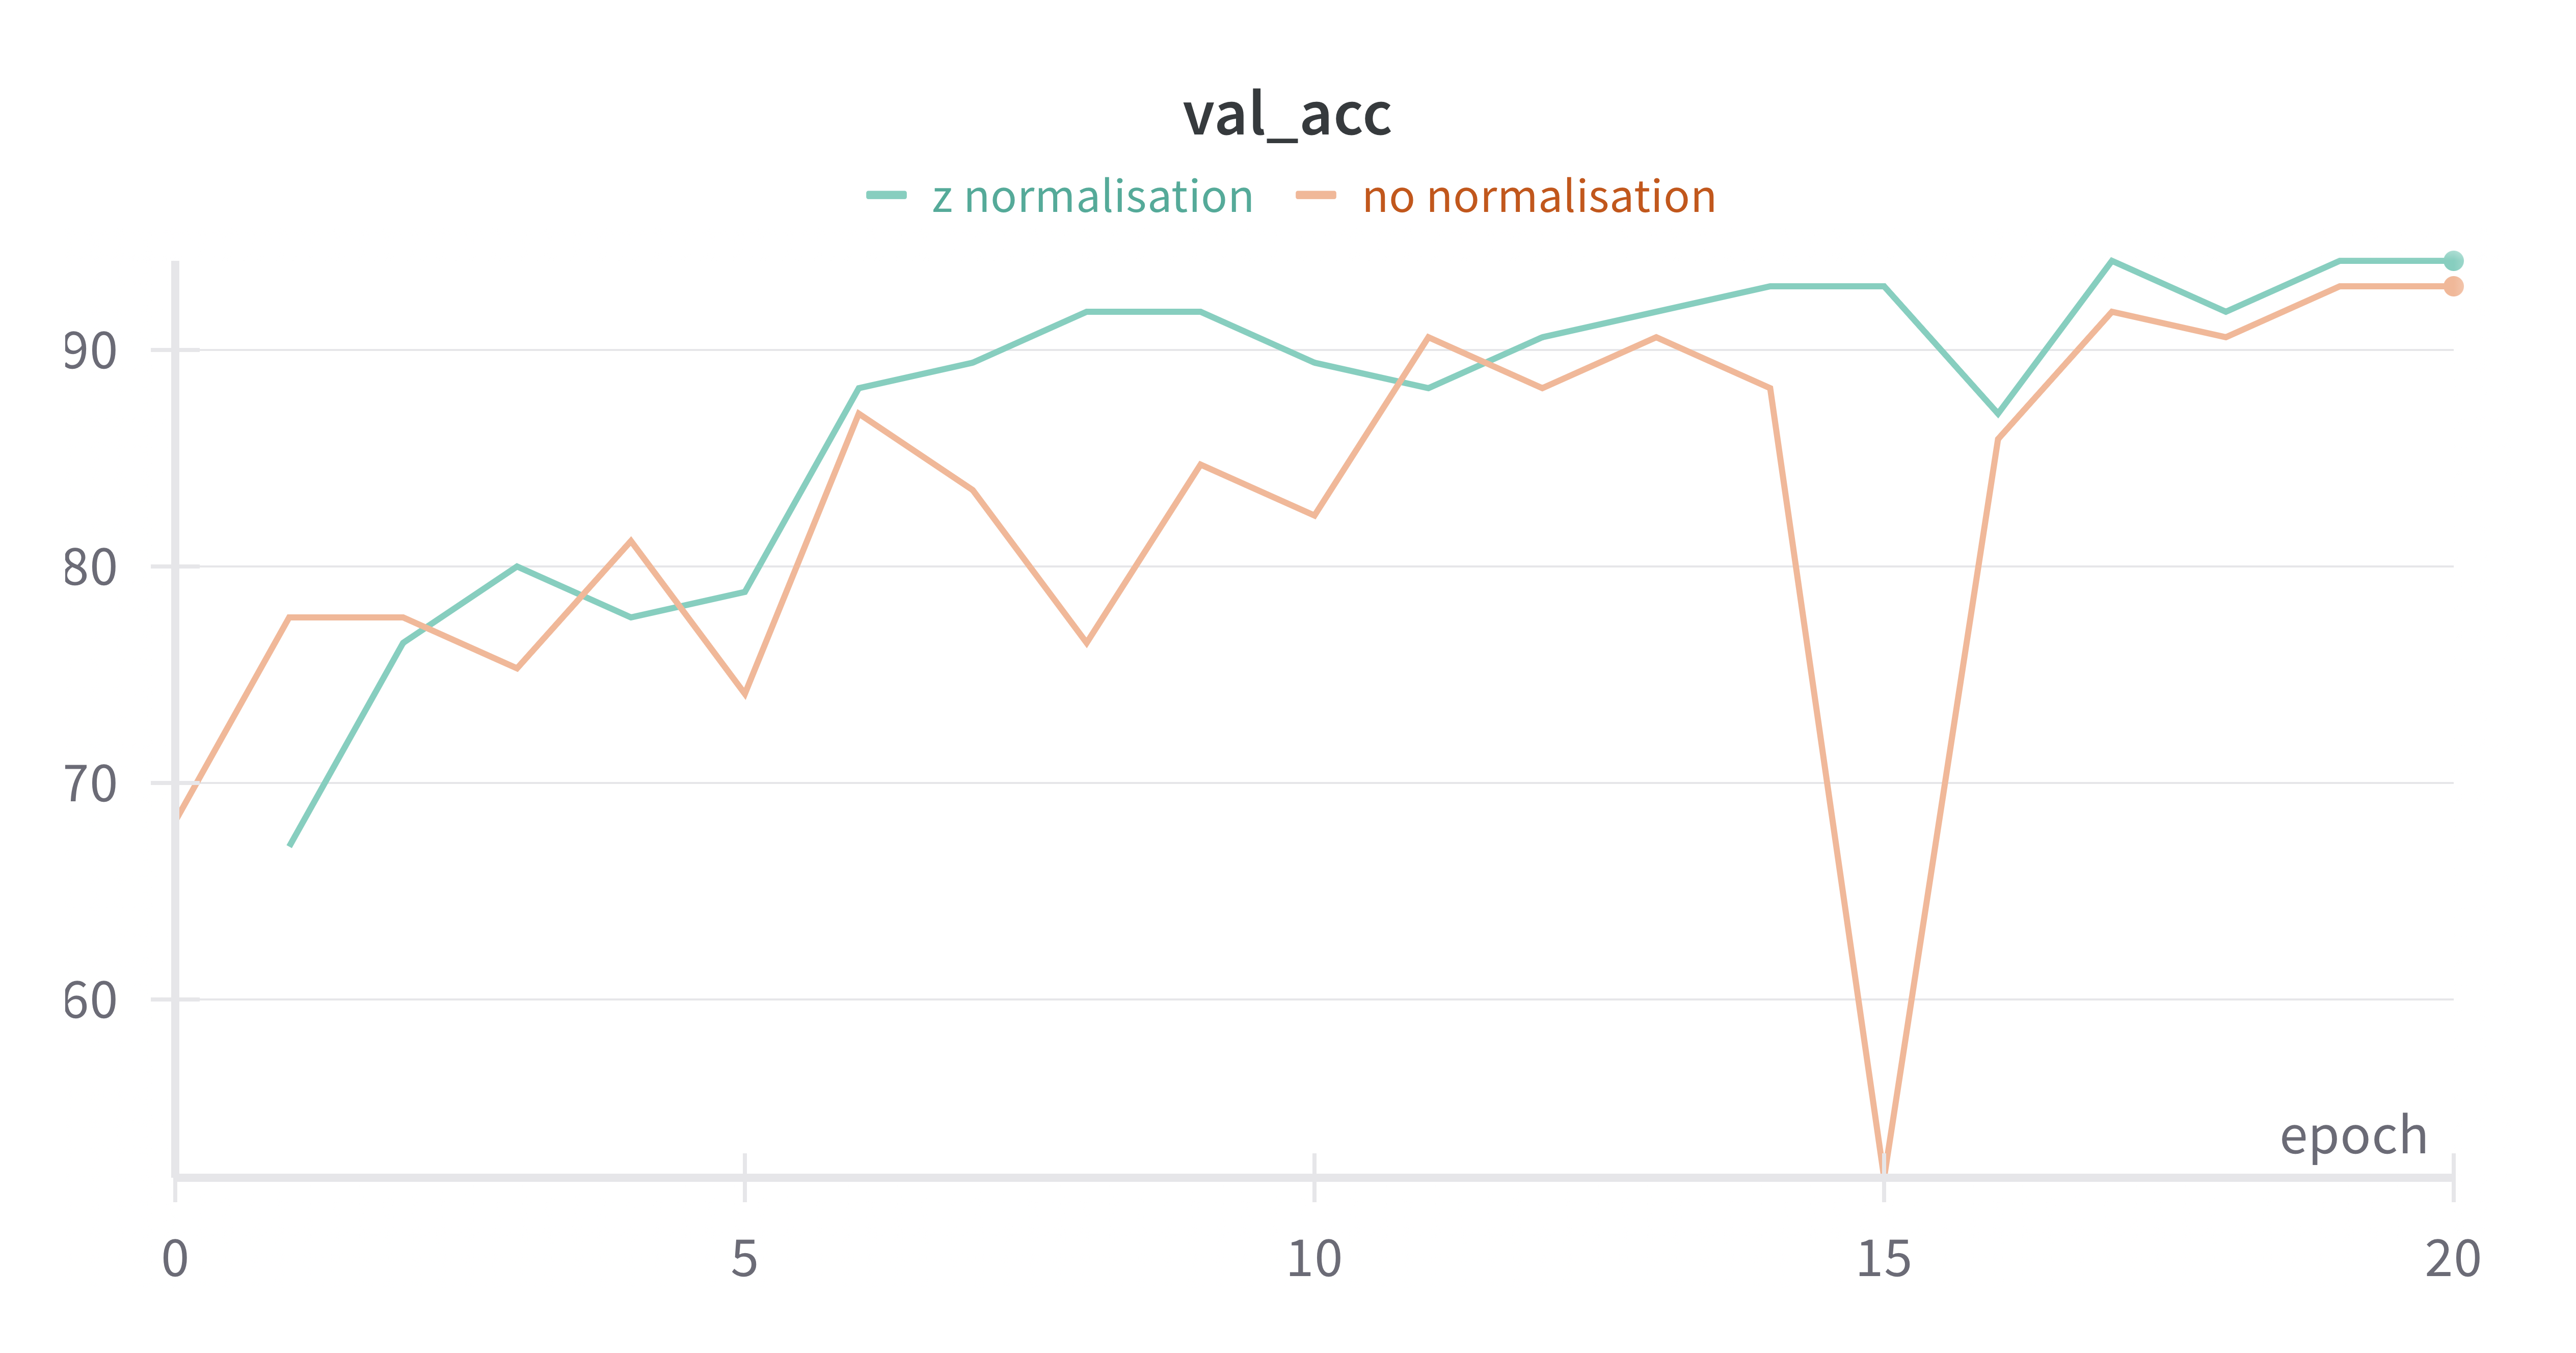
\includegraphics[width=\textwidth]{figures/znorm_val_acc.png}
  \caption{Validation accuracy over epochs with and without normalisation in the augmentation, demonstrating normalisations effectiveness in enhancing model generalization.}
  \label{fig:normalisation_accuracy}
\end{figure}

The optimal strategy (random noise + gamma adjustment + Z-normalization) improved validation accuracy by $\sim$5\% compared to using no augmentation, while the addition of geometric transformations (rotations, flips) not only failed to improve performance, as they all remaied within ±2\% but significantly increased training time from $\sim$5 to $\sim$20 epochs for comparable convergence.

\subsubsection{Group Leakage Impact}

The methodological investigation into group leakage (subject-level vs. scan-level partitioning) confirmed previous findings about inflated performance metrics. As shown in Figure \ref{fig:group_leakage}, scan-level partitioning produced artificially high accuracy (>90\%) compared to the more realistic subject-level isolation (77\%), demonstrating the critical importance of proper validation methodology in neuroimaging studies. We see one model with complete group leakage (scan-level), one with no group leakage (subject-level), and one with partial group leakage (train and val sets have some overlap). The model with complete group leakage achieved a test accuracy of 97.67\%, while the model with no group leakage achieved an accuracy of 70.28\%. The model with partial group leakage achieved an accuracy of 79.57\%.

\begin{figure}[htbp]
  \centering
  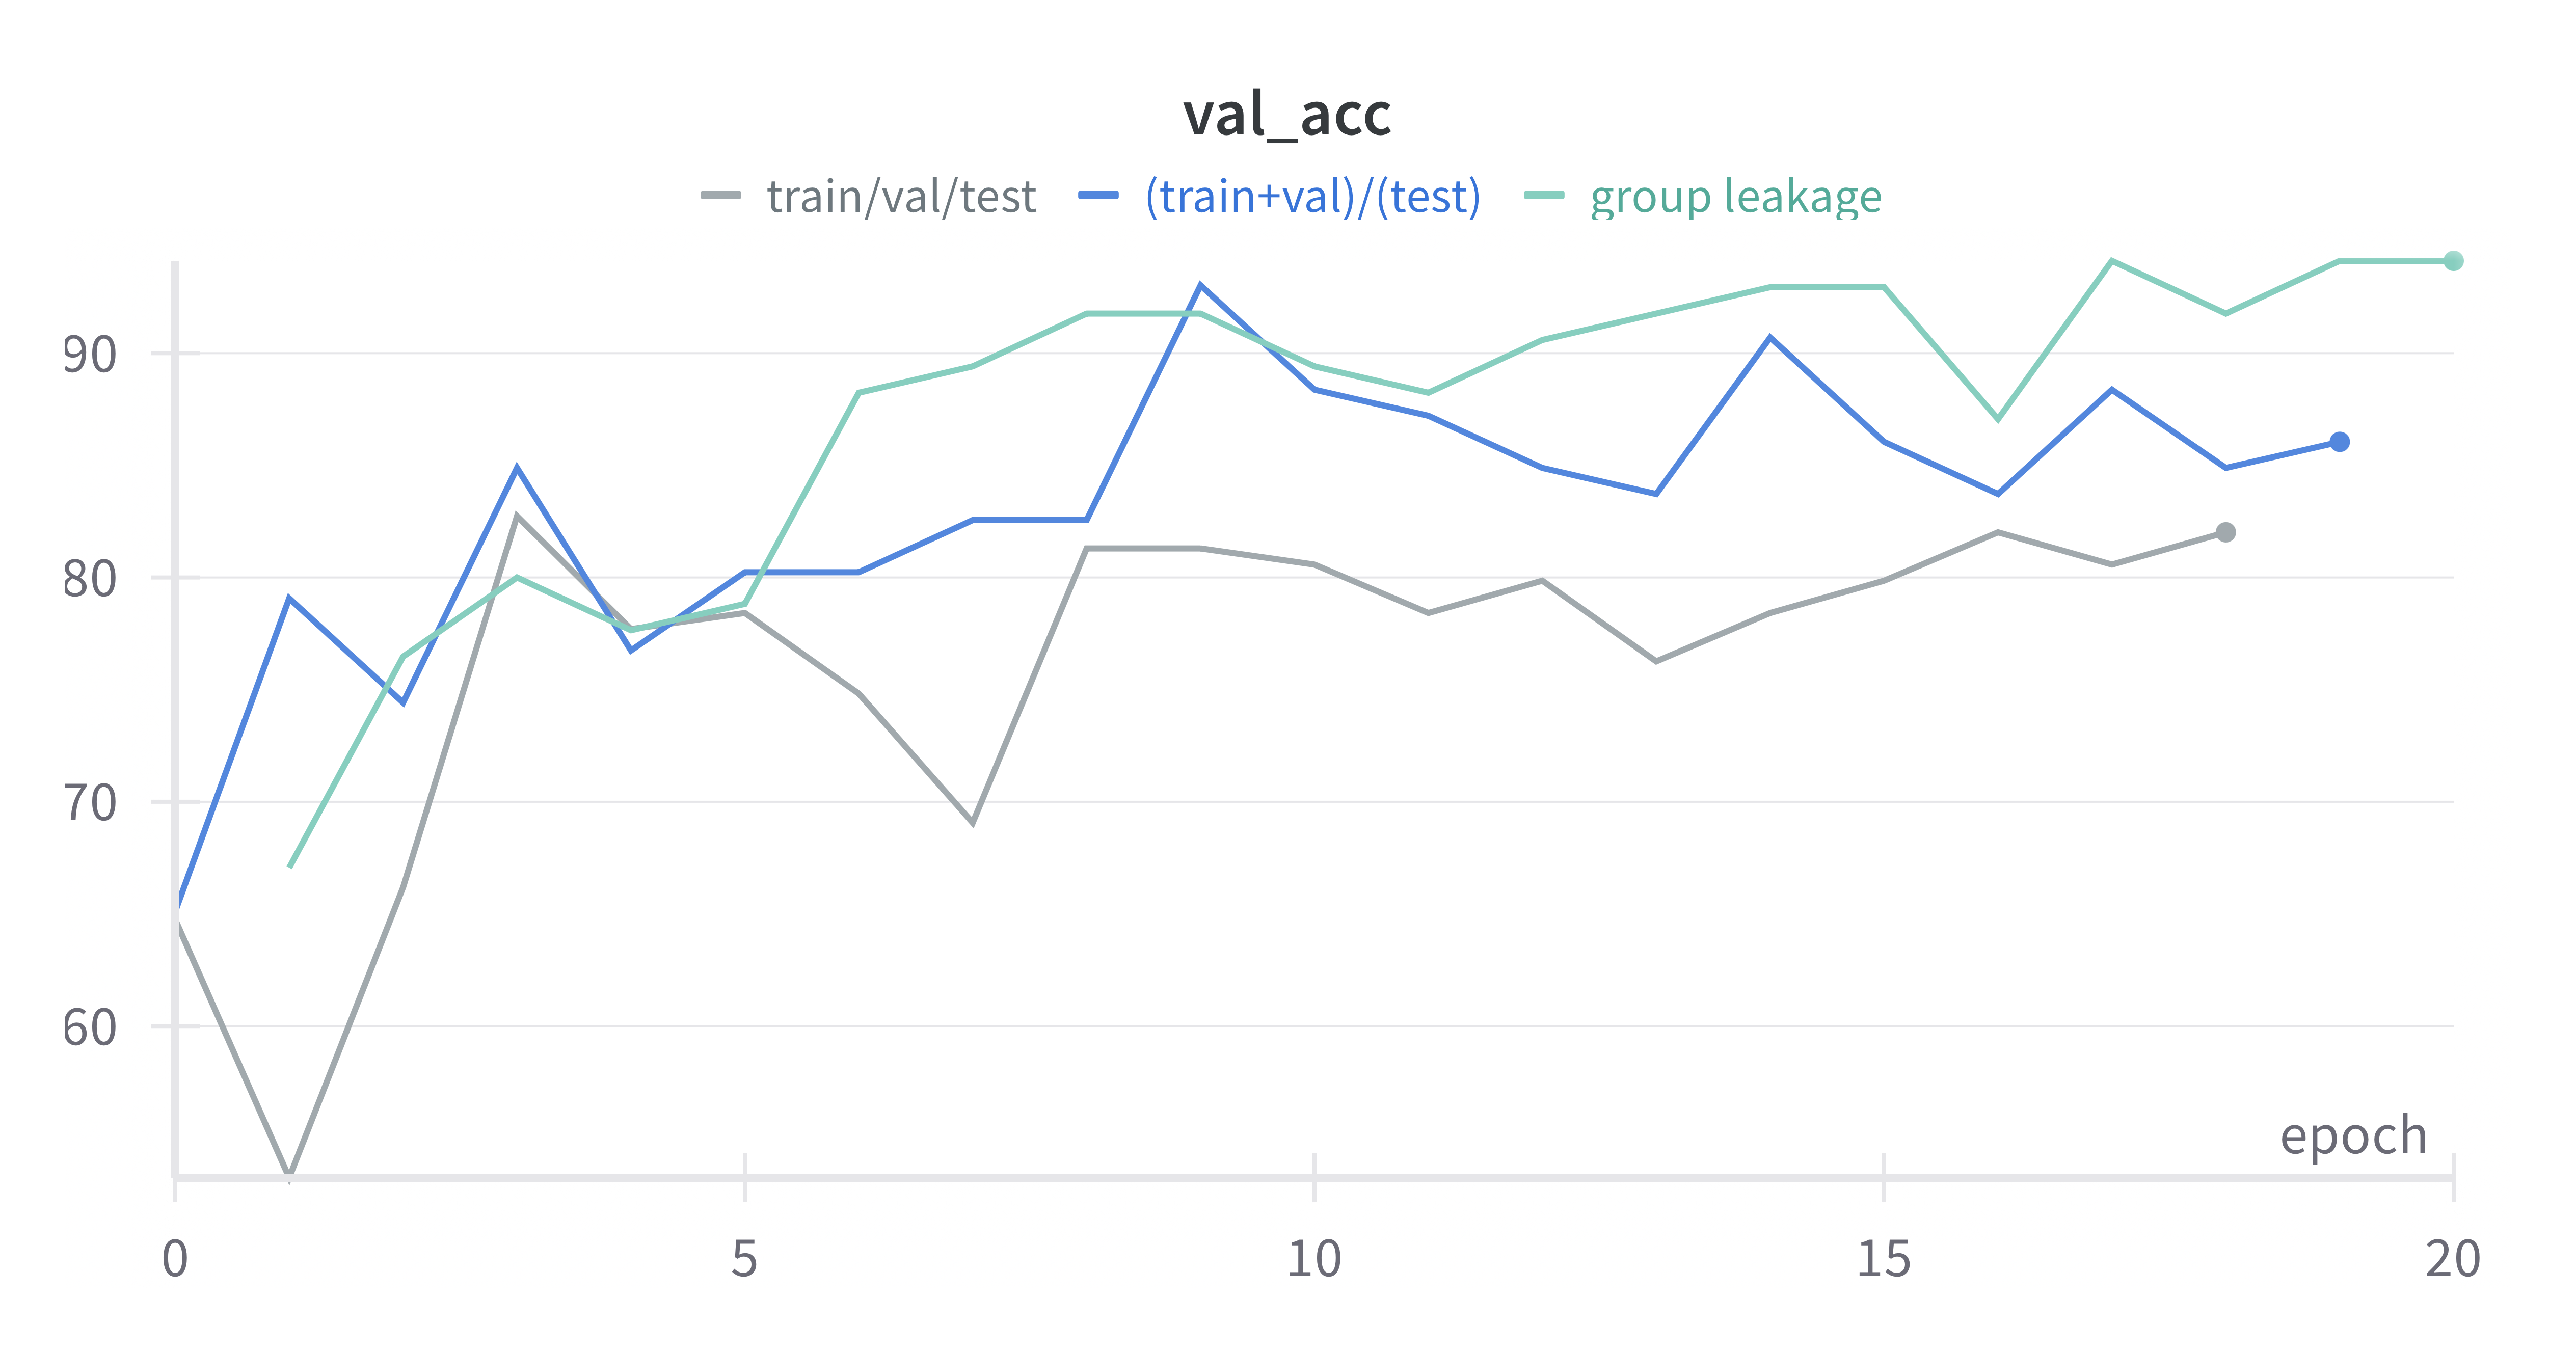
\includegraphics[width=\textwidth]{figures/leakage.png}
  \caption{Performance comparison between scan-level partitioning and subject-level isolation}
  \label{fig:group_leakage}
\end{figure}

This 20-percentage-point difference highlights the critical importance of proper validation methodology in neuroimaging studies and suggests that previously published results may be significantly overestimated if they employed scan-level partitioning.

\subsection{Explicable AI}
% TODO Visualization of model attention/activation maps XAI

\section{Discussion}
\label{sec:discussion}

This section critically examines the implications of these findings on transfer learning for Alzheimer's disease detection, contextualizing the results within existing literature while considering technical insights, clinical relevance, and methodological contributions.

\subsection{Interpretation of Results}

\subsubsection{Performance Metrics and Clinical Context}

The R3D-18 model achieved 77.26\% test accuracy with balanced performance across precision (77.1\%), recall (79.29\%), and specificity (75.33\%), indicating the model does not disproportionately favor either diagnostic category. This balance makes it suitable for clinical screening applications where both false positives and negatives carry significant consequences.

The ROC-AUC of 0.86 indicates good discriminative ability across classification thresholds, falling within the "good" range (0.8-0.9) in diagnostic test evaluation frameworks~\cite{mandrekar2010receiver}. The narrow standard deviation in accuracy across cross-validation folds (±2.34\%) suggests robust generalization, though the wider variation in recall (±16.01\%) warrants attention, indicating less consistent sensitivity across different subject groups.

Learning curves showed relatively rapid convergence (4-8 epochs), attributable to transfer learning initialization. This suggests that despite the substantial domain shift from video action recognition to neuroimaging, pre-trained feature extractors provide a valuable foundation for identifying neuroanatomical patterns.

While not meeting the ideal threshold for standalone diagnostic tools (typically >90\%), this performance offers clinical utility in several contexts: as a screening tool to prioritize specialist review, as assistive technology complementing human interpretation, and for longitudinal monitoring where relative assessments may prove more valuable than absolute classifications. This performance was achieved using structural MRI alone, without additional clinical data, cognitive assessments, or complementary modalities.

Several factors contribute to this performance ceiling. Disease heterogeneity is a primary factor, as structural changes in AD follow variable patterns, with overlap between normal aging and early AD~\cite{vemuri2010role}. Additionally, the reliance on structural changes presents limitations since structural alterations occur relatively late in the disease progression~\cite{jack2013tracking}, potentially limiting the discriminative ability of structural MRI alone. Despite the adaptive cropping strategy, resolution limitations are also a factor, as the 128³ resolution represents a significant reduction from native MRI resolution, potentially obscuring subtle differences.

\subsubsection{Comparison with Human Performance and Literature}

Contextualizing the model against human performance provides important perspective. Klöppel et al.~\cite{kloppel2008accuracy} found experienced neuroradiologists achieved $\sim$80\% accuracy in distinguishing AD from age-matched controls using structural MRI—comparable to the model's performance. However, radiologist performance drops considerably (to 63-70\%) when evaluating early-stage or atypical cases, highlighting a potential niche where algorithmic approaches might complement human expertise.

While the model's overall accuracy (77.26\%) is slightly below expert radiologist levels, its sensitivity (79.29\%) exceeds the reported average radiologist sensitivity of 70-75\%~\cite{frisoni2010clinical}, suggesting particular utility in reducing missed cases. The model's consistent performance contrasts with significant inter-reader variability in radiological assessment~\cite{kloppel2008accuracy}, suggesting potential for standardizing evaluations.

Performance appears lower than some published results, particularly those reporting >90\% accuracy. Key contributing factors include: stringent subject-level isolation methodology; dataset composition including challenging cases; and hardware constraints limiting resolution and model complexity. The 20-percentage-point difference observed between scan-level partitioning (97.67\% accuracy) and proper subject-level isolation (77.26\% accuracy) aligns with Davatzikos et al.'s~\cite{davatzikos2019machine} warning that data leakage can inflate performance by 10-15\%, suggesting many published results may be substantially overestimated.

Notably, these results align closely with Gunawardena et al.~\cite{gunawardena2017applying}, who employed similarly rigorous validation and reported 78.8\% accuracy, suggesting the approach yields realistic performance estimates for this challenging classification task.

\subsubsection{Analysis of Classification Errors}

Examining misclassified cases provides insight into model limitations. Analysis revealed approximately balanced errors: 21\% false negatives (AD classified as CN) and 25\% false positives (CN classified as AD).

False negatives ($\sim$20.71\% of AD cases) represent missed diagnostic opportunities. These may potentially represent subtle or atypical AD presentations, which would align with Jack et al.'s~\cite{jack2013tracking} observation that $\sim$10-20\% of AD cases present with atypical atrophy patterns. The literature suggests that cases with focal atrophy or predominantly temporal lobe involvement rather than classic widespread patterns are particularly challenging for both human raters and automated systems~\cite{kloppel2008accuracy}.

False positives ($\sim$24.67\% of CN cases) could lead to unnecessary treatment or psychological burden, potentially representing cases with age-related atrophy mimicking AD-related changes. The literature indicates annual atrophy rates of 1-2\% in normal aging versus 3-6\% in AD~\cite{vemuri2010role}, creating a challenging gray area for distinction. Boundary cases where age-associated atrophy resembles neurodegenerative patterns have been reported as common sources of diagnostic uncertainty in clinical practice~\cite{frisoni2010clinical}.

Despite preprocessing standardization, image quality variations have been shown in previous studies to impact classification performance~\cite{davatzikos2019machine}. Future work could include formal analysis of misclassified cases to identify whether specific demographic, clinical, or image acquisition factors contribute to classification errors.

\subsection{Technical Insights and Challenges}

\subsubsection{Transfer Learning Effectiveness}

The adaptation of video-pretrained models to MRI classification demonstrated viable cross-domain knowledge transfer despite fundamental differences between spatiotemporal video data and static volumetric MRI. This transfer proved non-trivial, requiring a balanced layer freezing strategy—preserving 25\% of parameters while fine-tuning 75\%—rather than the more extreme approaches common in natural image transfer learning. Notably, attempting to train only the final fully connected layer resulted in complete training failure with numerical instabilities, highlighting the substantial domain shift between video recognition and MRI analysis.

Despite this domain gap, models converged relatively quickly (5-8 epochs), suggesting that low-level features learned from video data remain useful for identifying structural patterns in brain MRI. The implementation of differential learning rates for newly initialized layers (10× higher) proved critical, allowing aggressive adaptation at the task-specific layers while making conservative updates to pretrained feature extractors.

These findings indicate that while video-to-MRI transfer is viable, the domain shift necessitates substantial adaptation rather than the "lightweight" fine-tuning often sufficient in natural image transfer applications.

\subsubsection{Dimensional Processing Impact}

A clear performance progression emerged across architectures with different approaches to dimensional processing. The fully 3D convolutional approach (R3D-18) consistently outperformed both mixed convolution (MC3-18) and factorized convolution (R(2+1)D-18) architectures, with performance declining as architectures incorporated more 2D elements. This strongly suggests that preserving complete volumetric spatial context is crucial for detecting the subtle structural patterns characteristic of neurodegenerative disease.

Contrary to findings in video classification tasks—where factorized convolutions often improve performance through increased non-linearities—our results demonstrate that spatial continuity preservation offered by pure 3D convolutions outweighs these theoretical advantages for structural MRI analysis. This insight challenges the common practice of processing MRI data as independent 2D slices and suggests prioritizing fully 3D approaches, particularly when targeting structural abnormalities with inherently 3D manifestations like hippocampal atrophy.

\subsubsection{Computational Challenges and Solutions}

The implementation revealed counterintuitive efficiency patterns: despite theoretical computational advantages of mixed and factorized convolutions, R3D-18 demonstrated substantially faster training times (1 hour/epoch) compared to MC3-18 (4 hours/epoch) and R(2+1)D (5 hours/epoch). This unexpected efficiency can be attributed to optimized implementations of standard 3D convolutions in modern deep learning frameworks. These findings challenge the assumption that architecturally "lighter" models necessarily translate to computational efficiency gains in practice.

Working with high-dimensional volumetric data (128×128×128) placed considerable demands on memory management. Batch size was restricted to 2 samples due to memory limitations, and several optimization techniques were necessary:

\begin{itemize}
    \item Setting gradients to \texttt{None} rather than zero reduced memory fragmentation
    \item Explicit cache clearing for Metal Performance Shaders prevented cumulative memory leakage
    \item Pre-trained weights reduced convergence time from 30+ epochs to 5-10 epochs
    \item Differential learning rates accelerated task-specific adaptation
    \item Dual-criterion early stopping saved approximately 40\% of potential training time
\end{itemize}

Despite these optimizations, the total training time of approximately 20 hours per run on consumer-grade hardware (M1 Mac) remained a significant constraint, limiting hyperparameter exploration and architectural comparison. Memory constraints prevented implementation of state-of-the-art volumetric Vision Transformers like MViT which required an estimated >32GB of memory.

These technical insights suggest several directions for future research: development of memory-efficient 3D architectures specifically designed for volumetric medical imaging; exploration of progressive resolution techniques enabling higher effective resolution while maintaining manageable memory footprints; and implementation of model quantization and pruning to enable deployment of more powerful architectures on consumer hardware.

% TODO
% \subsection{Model Interpretability}
% Things to consider:
%   - Insights from XAI analysis
%   - Visualization techniques for model attention/activation
%   - Correlation with known AD-affected regions
%   - Clinical relevance of identified features

\subsubsection{Data Leakage Prevention}

Perhaps the most methodologically significant challenge was preventing data leakage—a subtle but crucial issue in longitudinal medical imaging studies. Subject-level isolation revealed more realistic performance ($\sim$77\%) compared to scan-level partitioning (>90\% artificially inflated accuracy). Comprehensive subject tracking ensured complete isolation between dataset partitions, and partition-specific normalization prevented subtle forms of information leakage.

This finding represents a key methodological contribution, highlighting how implementation details dramatically impact reported effectiveness of deep learning approaches in medical imaging.

\subsection{Clinical Implications}

With a test accuracy of 77.26\%, the model shows potential as a screening or assistive mechanism rather than a standalone diagnostic tool. This performance should be contextualized against both rigorous subject-level validation methodology and clinical diagnostic accuracy for AD (65-96\%)~\cite{kloppel2008accuracy}.

\subsubsection{Potential Applications and Workflow Integration}

The model offers several advantages over manual assessment: standardized evaluations with quantifiable uncertainty measures; scalability to address increasing demands on radiology departments; and balanced precision-recall characteristics suitable for clinical screening. Its moderate computational requirements enable deployment beyond specialized research centers to community hospitals where neurological assessment expertise may be limited.

Integration into clinical practice could take several forms. The system could function as a triage mechanism generating AD probability scores to prioritize high-risk cases for specialist assessment. PACS integration would allow automatic processing of incoming scans, with results available alongside conventional images. It could also serve as an on-demand second-opinion service for cases with diagnostic uncertainty, or as a complementary quantitative biomarker within existing diagnostic frameworks that integrate cognitive assessments and other biomarker analyses.

The most promising application may be as part of multimodal diagnostic approaches when combined with CSF biomarkers ($A\beta$ and $tau$) and cognitive assessments. The AUC of 0.86 indicates good discriminative capability that could enhance clinical decision-making.

For longitudinal monitoring, automated analysis offers standardized assessment free from inter-reader variability~\cite{kloppel2008accuracy}. The model's ability to process full volumetric data may enable detection of subtle atrophy patterns across distributed brain regions before they manifest as observable symptoms, improving evaluation of disease progression and treatment response as disease-modifying therapies emerge.

\subsubsection{Implementation Barriers}

Several challenges must be addressed before clinical deployment. Regulatory approval with clear guidelines for the intended use and limitations is essential, alongside assessment in a prospective clinical setting to measure real-world performance and workflow impact. Development of robust transparency mechanisms in the decision-making process will be necessary to build clinician trust, while integration with diverse PACS and electronic health record platforms will require technical standardization. Clear guidelines on the role of automated analysis in the diagnostic process must also be established to ensure appropriate use.

A realistic timeline would suggest 2-3 years for validation and regulatory processes before initial clinical deployment could begin, with longitudinal monitoring required to assess clinical impact on diagnostic accuracy and patient outcomes.

From an economic perspective, early diagnosis through automated screening could potentially reduce healthcare costs through earlier intervention and more appropriate care planning~\cite{jack2018nia}. The system could improve referral appropriateness and enhance value extraction from existing MRI data without additional imaging costs.

\subsection{Limitations}

\subsubsection{Dataset and Classification Limitations}

The exclusive use of the ADNI dataset introduces potential biases that may affect generalizability. ADNI's demographic composition skews toward higher education levels and predominantly Caucasian participants, potentially limiting generalizability across populations where AD presentation and progression may differ~\cite{jack2008alzheimer}. The dataset's stringent inclusion criteria potentially exclude patients with significant comorbidities, vascular pathology, or mixed dementia that are common in clinical practice. Despite augmentation attempts, inter-scanner and inter-site variations remain a concern, potentially introducing confounding technical factors. Furthermore, focusing on AD versus CN excludes borderline and early-stage presentations, limiting the model's applicability across the disease spectrum.

The binary classification approach (AD vs. CN) represents another significant limitation. By excluding Mild Cognitive Impairment, the approach bypasses critical early-stage detection challenges where intervention might be most beneficial. The lack of differential diagnosis capability between various dementia types (e.g., vascular dementia, Lewy body dementia) substantially limits clinical utility in real-world settings where multiple pathologies often co-exist. This binary framing also misrepresents the continuous progression from normal aging to severe dementia, artificially dichotomizing what is typically a gradual process. Additionally, mixed pathologies commonly seen in clinical practice remain unaddressed by this simplified diagnostic model.

\subsubsection{Technical and Methodological Limitations}

Resolution and modality limitations affected the model's discriminative capabilities. The 128³ resolution represents a substantial reduction from native MRI resolution, potentially obscuring fine-grained differences. Additionally, relying solely on T1-weighted structural MRI ignores complementary information available from other sequences and modalities that could enhance diagnostic accuracy.

The transfer learning approach introduces fundamental limitations to the methodology. Features optimized for video action recognition are inherently different from the structural patterns relevant in AD detection, potentially limiting the effectiveness of knowledge transfer across these disparate domains. The layer freezing strategy implemented represents just one of many possible transfer learning approaches; more sophisticated adaptation methods might better bridge the domain gap and improve performance. The fundamental mismatch between video classification (where temporal dynamics are crucial) and structural MRI analysis (where static volumetric patterns are key) may ultimately limit knowledge transfer effectiveness, potentially explaining the performance ceiling observed in the experiments.

\subsubsection{Validation and Deployment Limitations}

The retrospective nature of this study presents inherent limitations for clinical translation. Testing was performed exclusively on ADNI data with its standardized acquisition protocols that may not reflect the variability encountered in routine clinical settings. External validation across diverse datasets is essential for assessing real-world performance across different populations, scanners, and acquisition parameters. The retrospective analysis does not capture prospective performance in a clinical workflow, where factors like acquisition variability and patient selection significantly impact utility. While 3-fold cross-validation provided some assessment of generalizability, more extensive validation across different acquisition sites or protocols would strengthen confidence in the robustness of the approach. The model's performance (77.26\% accuracy), while promising, falls short of the threshold typically considered necessary for independent clinical applications (>90\%), limiting its immediate translational potential to assistive rather than autonomous functions. Additionally, direct comparison with radiologist performance on the same test set was not performed, which would have provided valuable context for the model's relative clinical utility compared to human experts.

% \subsubsection{Interpretability and Explainability Limitations}
% % TODO once XAI is done redo this
% Despite visualization attempts, several interpretability limitations remain:

% \begin{itemize}
%     \item \textbf{Limited explainability}: The current implementation offers limited insight into specific decision-making processes beyond visualization of attention regions. This "black box" nature presents barriers to clinical acceptance.
    
%     \item \textbf{Region-specific interpretations}: The lack of feature-specific interpretation (e.g., quantification of specific regional atrophy patterns and their contribution to classification) limits the model's ability to provide clinically actionable insights beyond binary classification.
    
%     \item \textbf{Threshold determination}: The optimal decision threshold for clinical use remains undetermined, with different thresholds potentially appropriate for screening versus diagnostic confirmation contexts.
    
%     \item \textbf{Confidence calibration}: The model outputs probability scores that may not be well-calibrated to actual diagnostic confidence, potentially misleading clinical interpretation without proper calibration procedures.
% \end{itemize}

These limitations collectively suggest several promising directions for future research, including architectural innovations specifically designed for volumetric medical data, multimodal approaches integrating complementary imaging sequences, and more comprehensive validation strategies that better approximate clinical deployment conditions.

\section{Conclusions}
\label{sec:conclusions}

\subsection{Summary of Findings and Contributions}

This dissertation investigated the efficacy of adapting deep learning models, originally designed for video action recognition, for the challenging task of Alzheimer's disease (AD) detection using structural Magnetic Resonance Imaging (MRI). Motivated by the pressing need for automated, reliable tools to aid in early AD diagnosis and the limitations of existing approaches, particularly concerning data scarcity and methodological rigor in neuroimaging AI, this work systematically evaluated a specific transfer learning paradigm: leveraging models pre-trained on large-scale video datasets (Kinetics-400) for volumetric MRI classification. The research aimed to address key questions regarding the feasibility of this approach, the optimal 3D convolutional architectures, the impact of specific preprocessing choices, and the critical importance of methodologically sound validation practices.

The primary contribution of this work lies in demonstrating the viability and characterizing the performance of transferring knowledge from the video domain to volumetric neuroimaging for AD classification. The optimized R3D-18 model, a fully 3D convolutional architecture pre-trained on Kinetics-400 and fine-tuned on ADNI data, achieved a respectable test accuracy of 77.26\% and an AUC-ROC of 0.86 for binary AD versus Cognitively Normal (CN) classification. This performance, achieved using only structural MRI data and validated with strict subject-level isolation, suggests that features learned for recognizing spatio-temporal patterns in videos can be effectively adapted to identify the static, volumetric structural changes characteristic of AD, such as hippocampal and cortical atrophy. While not reaching the levels required for standalone diagnosis, this result positions the approach as a potentially valuable assistive tool within a clinical workflow, comparable in accuracy to non-expert human readers and potentially exceeding average sensitivity.

A significant technical insight emerged from the comparative analysis of different 3D architectural variants derived from the video domain. Experiments consistently showed that the fully 3D convolutional architecture (R3D-18) outperformed hybrid (MC3-18) and factorized (R(2+1)D-18) approaches. This finding underscores the critical importance of preserving complete volumetric spatial context when analyzing structural MRI for neurodegenerative patterns. It challenges the notion that computationally lighter architectures, which compromise full 3D processing, are necessarily superior or even equivalent for this specific task, suggesting that the subtle, distributed nature of AD-related atrophy benefits significantly from undiluted 3D feature extraction. This provides strong empirical support for prioritizing fully 3D architectures in future neuroimaging AI development for structural analysis.

Furthermore, this research highlights the substantial impact of preprocessing choices on model performance within a transfer learning context. The development and evaluation of a bespoke preprocessing pipeline, featuring state-of-the-art skull stripping (SynthStrip), intensity normalization (Z-score), and a novel adaptive cropping strategy, proved crucial. The adaptive cropping method, designed to maximize effective resolution within computational constraints (128³ volume size), demonstrated a tangible benefit over naive downsampling, emphasizing the need to preserve anatomical detail, particularly in critical regions like the hippocampus. Notably, the deliberate omission of spatial normalization to a standard template, aimed at preserving native atrophy patterns potentially distorted by registration, did not hinder performance and aligns with emerging evidence suggesting deep learning models can effectively learn from native-space data. The minimal yet effective data augmentation strategy (noise, gamma, normalization) further refined the model's robustness.

Perhaps the most critical methodological contribution of this dissertation is the empirical demonstration and quantification of the impact of data leakage in neuroimaging AI evaluation. Initial experiments using conventional scan-level partitioning yielded artificially inflated accuracy metrics exceeding 90\%, mirroring potentially optimistic results in some published literature. Implementing strict subject-level isolation, ensuring no individual subject's data appeared across training, validation, and test sets, resulted in a more realistic accuracy of 77.26\%. This ~20 percentage point discrepancy starkly illustrates the pitfalls of inadequate validation and reinforces the absolute necessity of rigorous, subject-aware data splitting protocols for obtaining trustworthy performance estimates in medical imaging, particularly when dealing with longitudinal datasets like ADNI. This finding serves as a crucial reminder for the field to prioritize methodological transparency and rigor to ensure the development of genuinely generalizable and clinically reliable AI tools.

\subsection{Limitations}

Despite the promising results, this study is subject to several limitations that pave the way for future research. The reliance on the ADNI dataset, while providing high-quality standardized data, introduces potential demographic and clinical biases and may not fully represent the heterogeneity encountered in real-world clinical practice. The binary classification task (AD vs. CN) simplifies the complex spectrum of cognitive decline, omitting the crucial Mild Cognitive Impairment (MCI) stage, which is a key target for early intervention. Future work should focus on multi-class classification (CN vs. MCI vs. AD) and differential diagnosis against other dementia types. The performance achieved, while significant, indicates room for improvement, potentially through exploring more advanced architectures, integrating complementary data modalities, or refining transfer learning strategies.

Technical limitations, primarily imposed by computational resources (consumer-grade M1 Mac), restricted the exploration of larger models (like deeper ResNets or Vision Transformers) and higher input resolutions. Future investigations with access to greater computational power could explore these avenues, potentially unlocking higher performance. The inherent domain gap between video action recognition and static MRI analysis, while shown to be bridgeable, may still impose a ceiling on transfer learning effectiveness; exploring self-supervised pre-training directly on large medical imaging datasets could offer a complementary or superior approach. Furthermore, the interpretability of the model remains limited, necessitating future work on incorporating advanced Explainable AI (XAI) techniques to elucidate the model's decision-making process and build clinical trust.

\subsection{Future Directions}

Future directions should prioritize external validation on diverse, multi-site datasets to assess real-world generalizability. Extending the framework to longitudinal analysis, tracking changes over time within individuals, holds significant promise for monitoring disease progression and treatment response. Incorporating multimodal data, such as PET imaging, diffusion tensor imaging (DTI), CSF biomarkers, genetic information, and clinical/cognitive scores, is likely essential for pushing diagnostic accuracy towards clinically actionable levels. Architectural innovation focused on memory-efficient 3D networks or hybrid approaches specifically designed for medical imaging could also yield performance gains. Finally, prospective clinical validation studies are indispensable for evaluating the true clinical utility and impact of such AI tools within existing diagnostic workflows.

In conclusion, this dissertation provides compelling evidence for the potential of adapting video-pretrained 3D convolutional neural networks for Alzheimer's disease detection from structural MRI, contributing to the growing field of AI in medical imaging. It highlights the importance of preserving full volumetric context for analysing neurodegenerative patterns and underscores the substantial benefits of optimized, native-space preprocessing pipelines. Critically, it offers a stark, quantitative demonstration of the necessity for adhering to stringent methodological validation standards, particularly subject-level data isolation, serving as a vital reminder for the research community to prioritize transparency and rigor to ensure the reliability and reproducibility of AI research in healthcare. While acknowledging the limitations and the performance gap still needing to be bridged for standalone diagnostic use, the achieved results demonstrate the promise of this transfer learning approach. Tools developed from this line of research, once sufficiently validated and refined, could serve as valuable assistive technologies, helping to standardize MRI interpretation, reduce inter-reader variability, and potentially flag subtle cases for expert review. Continued research, focusing on methodological soundness, external validation, multimodal integration, and careful consideration of ethical implications and clinical integration pathways, will be key to translating this potential into tangible benefits for patients and healthcare systems facing the global challenge of Alzheimer's disease.

\bibliographystyle{IEEEtran}
\bibliography{references} 

\appendix

% - **Detailed Implementation Specifics**

%   - Code snippets for key components
%   - Hyperparameter configurations
%   - Detailed architectures

% - **Additional Visualizations**

%   - Extended results tables
%   - Additional performance metrics
%   - Sample preprocessing visualizations
%   - Extended XAI visualizations

% - **Computational Resources Analysis**
%   - Detailed training times
%   - Memory usage patterns
%   - Optimization attempts


\end{document}



